\documentclass[12pt, a4paper]{report}

% Pass hyperref options safely
\PassOptionsToPackage{breaklinks}{hyperref}

\usepackage{graphicx} % For including images
\usepackage{titlesec} % For customizing section titles
\usepackage{tocloft} % For customizing table of contents
\usepackage{acro} % For acronyms

%% ____Bibliography____%%
\usepackage[numbers,sort&compress]{natbib}
\usepackage{amsmath}
% Page margins
\usepackage[left=1.5in, right=1in, top=1in, bottom=1in]{geometry}
% Hyperlinks (LOAD ONCE, LOAD LAST)
\usepackage{hyperref}
\usepackage{float}
\usepackage{placeins}
\usepackage{xcolor}     % for \rowcolor
 \usepackage{colortbl}   % for row shading
 \usepackage{makecell}   % for \makecell and \thead
\definecolor{gapgray}{gray}{0.92}

\usepackage{comment}
\usepackage{algorithm}
% \usepackage{algorithmic}
\usepackage{algpseudocode}
\usepackage{soul}    % in preamble


%\hypersetup{colorlinks=true,citecolor=blue,linkcolor=blue,urlcolor=blue}


% Remove page number from the first page
\thispagestyle{empty}

% Customize table of contents, list of figures, and list of tables
\renewcommand{\cfttoctitlefont}{\hfill\Large\bfseries}
\renewcommand{\cftaftertoctitle}{\hfill}
\renewcommand{\cftloftitlefont}{\hfill\Large\bfseries}
\renewcommand{\cftafterloftitle}{\hfill}
\renewcommand{\cftlottitlefont}{\hfill\Large\bfseries}
\renewcommand{\cftafterlottitle}{\hfill}

% This is my customize variable
\newcommand{\mypar}{\vspace{0.8em}\noindent} 

% Define acronyms
% Define acronyms
\DeclareAcronym{ITS}{
	short = ITS,
	long = Intelligent Transportation Systems
}
\DeclareAcronym{VANET}{
	short = VANET,
	long = Vehicular Ad Hoc Network
}
\DeclareAcronym{V2V}{
	short = V2V,
	long = Vehicle-to-Vehicle
}
\DeclareAcronym{V2I}{
	short = V2I,
	long = Vehicle-to-Infrastructure
}
\DeclareAcronym{SDVN}{
	short = SDVN,
	long = Software-Defined Vehicular Network
}
\DeclareAcronym{SDN}{
	short = SDN,
	long = Software-Defined Networking
}
\DeclareAcronym{AI}{
	short = AI,
	long = Artificial Intelligence
}
\DeclareAcronym{ML}{
	short = ML,
	long = Machine Learning
}
\DeclareAcronym{LLM}{
	short = LLM,
	long = Large Language Model
}
\DeclareAcronym{FL}{
	short = FL,
	long = Federated Learning
}
\DeclareAcronym{RSU}{
	short = RSU,
	long = Roadside Unit
}
\DeclareAcronym{IDS}{
	short = IDS,
	long = Intrusion Detection System
}
\DeclareAcronym{OSR}{
	short = OSR,
	long = Open-Set Recognition
}
\DeclareAcronym{DAE}{
	short = DAE,
	long = Deep Auto-Encoder
}
\DeclareAcronym{LSTM}{
	short = LSTM,
	long = Long Short-Term Memory
}
\DeclareAcronym{KNN}{
	short = KNN,
	long = K-Nearest Neighbor
}
\DeclareAcronym{GA}{
	short = GA,
	long = Genetic Algorithm
}
\DeclareAcronym{PDR}{
	short = PDR,
	long = Packet Delivery Ratio
}
\DeclareAcronym{E2E}{
	short = E2E,
	long = End-to-End
}

\DeclareAcronym{ANN}{
	short = ANN,
	long = Artificial Neural Network
}
\DeclareAcronym{RF}{
	short = RF,
	long = Random Forest
}
\DeclareAcronym{SVM}{
	short = SVM,
	long = Support Vector Machine
}
\DeclareAcronym{DSRC}{
	short = DSRC,
	long = Dedicated Short-Range Communications
}
\DeclareAcronym{VLC}{
	short = VLC,
	long = Visible Light Communication
}

\begin{document}


\thispagestyle{empty}

\begin{center}

\begin{center}
 
\includegraphics[width=2cm,keepaspectratio=true]{uor_logo.jpg}
 % uor_logo.jpg: 236x331 pixel, 72dpi, 8.33x11.68 cm, bb=0 0 236 331
\end{center}

\vspace{1.5cm}
\begin{huge}
%%%%%%%%%%%%%%%%%%%%%%%%%%%%%%%%%%%%%%%%%%%%%%%%%%%%
% Project title
%%%%%%%%%%%%%%%%%%%%%%%%%%%%%%%%%%%%%%%%%%%%%%%%%%%%
A Blockchain, Large Language Model, and Federated Learning based Secure Approach to Mitigate Grey Hole Attack in Software-Defined Vehicular Networks
%%%%%%%%%%%%%%%%%%%%%%%%%%%%%%%%%%%%%%%%%%%%%%%%%%%%
\end{huge} \\
\vspace{1cm}

\begin{normalsize}
An undergraduate project proposal report submitted to the
\end{normalsize}\\
\vspace{1cm}

\begin{large}
Department of Electrical and Information Engineering\\
Faculty of Engineering\\
University of Ruhuna\\
Sri Lanka
\end{large}\\

\vspace{1cm}

\begin{normalsize}in partial fulfillment of the requirements for the \end{normalsize}\\
\vspace{1cm}

\begin{large}\textbf{Degree of the Bachelor of the Science of Engineering Honours}\end{large}\\

\vspace{1cm}
\begin{normalsize}by  \end{normalsize}
\vspace{1cm}

\begin{tabular}[h]{lll}
 %%%%%%%%%%%%%%%%%%%%%%%%%%%%%%%%%%%%%%%%%%%%%%%%%%%%%%%%%%
 % Names and Registration Numbers
 %%%%%%%%%%%%%%%%%%%%%%%%%%%%%%%%%%%%%%%%%%%%%%%%%%%%%%%%%%
 D. Abenayaka	& - & 	EG/2021/4376\\
 B.M.L.P. Abesinghe	& - & 	EG/2021/4377\\
 I.G.N. Hasalanka	& - & 	EG/2021/4543\\
 H.E. Kularathna 	& - &	EG/2021/4619
 %%%%%%%%%%%%%%%%%%%%%%%%%%%%%%%%%%%%%%%%%%%%%%%%%%%%%%%%%%
\end{tabular}\\
\vspace{1cm}

%\date{June, 2009}
\vspace{1cm}

%%%%%%%%%%%%%%%%%%%%%%%%%%%%%%%%%%%%%%%%%%%%%%%%%%%%%%
% if one supervisor
%%%%%%%%%%%%%%%%%%%%%%%%%%%%%%%%%%%%%%%%%%%%%%%%%%%%%%%
%  .............................................. \\
% Prof. A.B.C. Dee\\
% (Supervisor)


%%%%%%%%%%%%%%%%%%%%%%%%%%%%%%%%%%%%%%%%%%%%%%%%%%%%
% If two supervisors
%%%%%%%%%%%%%%%%%%%%%%%%%%%%%%%%%%%%%%%%%%%%%%%%%%%%
\begin{tabular}[h]{lll}

	\begin{tabular}{c}
	.............................................. \\
	Dr. P.A.D.S.N. Wijesekara\\
	(Supervisor)
	\end{tabular}
&
	\begin{tabular}{c}
	.............................................. \\
	Mr. Samansiri De Silva\\
	(Co-Supervisor)
	\end{tabular}

\end{tabular}\\
% End of "If two supervisors


\end{center}

%%%%%%%%%%%%%%%%%%%%%%%%%%%%%%%%%%%%%%%%%%%%%%%%%%%%%%%%%%%%%%%%%%%%%%%%%%%%%%%%%%%%%%%%%%%%%%%%%%
% END OF FILE
%%%%%%%%%%%%%%%%%%%%%%%%%%%%%%%%%%%%%%%%%%%%%%%%%%%%%%%%%%%%%%%%%%%%%%%%%%%%%%%%%%%%%%%%%%%%%%%%%%


% This is my customize variable (this removed - commented)
% \setlength{\parindent}{0pt}   % No indentation
% \setlength{\parskip}{0.8em}   % Gap between paragraphs


\renewcommand{\thepage}{\roman{page}} % Start page numbering in roman

\chapter*{Abstract}
\begin{comment}
Software defined vehicular networks (SDVN) allow vehicles to communicate effectively although they are susceptible to gray hole attacks, which are malicious nodes that use selective packet dropping to disrupt on-traffic and safety. The Traditional approaches that are in use are not completely effective or work well since they are not trustful, flexible, and offer real time protection in dynamic networks (dynamic network).

\mypar
This project proposes a secure mechanism to locate and prevent gray hole attacks in SDVNs. The blockchain maintains an immutable, secure register of the actions of the nodes, thus everything is transparent and just. Large Language Models (LLMs) observe the patterns in the network in real-time to identify threats and generate intelligent solutions, such as new routing policies. Federated Learning allows vehicles to learn models collaboratively without exchanging personal information, enabling detection to be improved and privacy maintained.

\mypar
There are three attack scenarios in the system. They are fixed rate selective dropping, time based intermittent dropping and target specific intelligent gray hole attacks. NS3 and SUMO will be used to perform simulations and Hyperledger Fabric will be used to implement the blockchain.

\mypar
In this project, We will verify such key results as the ratio of packet delivery, latency and the reliability of the network in this project. This project aims at a helpful, secure and expandable system that will ensure SDVN communication is more dependable and secure to smart cities and self driving vehicles without malicious communication.
\end{comment}
% ============================================================
% REPLACE ABSTRACT
% ============================================================

Grey hole attacks in Software-Defined Vehicular Networks (SDVNs) present a
uniquely challenging security threat: malicious nodes selectively suppress
packet forwarding while mimicking normal mobility-induced packet loss, evading
detection across both the data plane and the SDN controller plane. Existing
solutions address only subsets of the attack space, omit controller-plane
vectors, and lack the post-quantum cryptographic protection and lightweight
deployability required for real-world vehicular deployment. This paper presents
SHIELD-GH, a dual-mode detection and mitigation framework that formalizes six
distinct grey hole attack signatures across two network planes and provides
both a rule-based lightweight mode and a full AI-cryptographic mode. The
lightweight mode employs mobility-corrected sliding-window signature detection
(covering fixed-rate, intermittent, and target-specific variants) with HMAC-based packet authentication for low-overhead deployment on resource-constrained vehicular nodes. The full mode integrates a fine-tuned Large Language Model (LLM) with a blockchain-verified Federated Learning (FL) aggregator for semantic anomaly detection, combined with post-quantum cryptographic mitigation using CRYSTALS-Kyber key encapsulation, CRYSTALS-Dilithium signatures, zk-SNARK-based packet forwarding proofs, and $(k,n)$-threshold signatures for collectively authorized node isolation. A novel Mobility-Aware Trust Decay (MATD) mechanism and a Dual-Evidence Blockchain Smart Contract (DEBSC) ensure that RSU handoff ambiguity does not inflate false positive rates. 

% Comment out this line as you don't have results yet.

% Simulation results in NS-3 with SUMO mobility traces and Hyperledger Fabric blockchain demonstrate that SHIELD-GH achieves a detection accuracy exceeding X\% across all six attack variants, with false positive rate below Y\%, while maintaining packet delivery ratio above Z\% and end-to-end delay within acceptable bounds for safety-critical vehicular applications.

\newpage

% Table of Contents
\tableofcontents
\newpage

% List of Figures
\listoffigures
\newpage

% List of Tables
\listoftables
\newpage

% Acronyms
\addcontentsline{toc}{chapter}{Acronyms} % Add to table of contents
\acuseall % Use all acronyms to ensure they appear in the list
\printacronyms
\newpage

\renewcommand{\thepage}{\arabic{page}} % Start page numbering in arabic 
\setcounter{page}{1} % start page numbering from 1

% Main Content
\chapter{Introduction}
\section{Background}

\subsection{Evolution of Vehicular Networks}
Intelligent Transportation Systems (ITS) have brought a new generation of connected vehicles, which is able to communicate with each other and roadside infrastructure. Vehicular Ad Hoc Networks (VANETs) were the foundation of early vehicular communication systems and provided simple vehicle-to-vehicle (V2V) and vehicle-to-infrastructure (V2I) communication. Nevertheless, VANETs have a number of challenges because of high vehicle mobility, high topology changes, and lack of centralized network control.

\mypar
Software-Defined Vehicular Networks (SDVNs) have been proposed in order to address these shortcomings by extending the concept of software defined networking to motor vehicle contexts. SDVNs decouple the control plane and data plane to enable centralized controllers to make routing decisions, traffic flow, and resource allocation more efficiently. This is a programmable and flexible architecture that is needed to support safety-critical ITS applications like collision avoidance systems, traffic management, and emergency response services. \cite{ieee10402120, islam2021sdvn}.


\subsection{Security Challenges and Grey Hole Attacks in SDVN}

Since SDVNs are becoming more and more significant in the context of road safety and autonomous driving, their safety and reliability have become one of the most significant concerns. The mobile nature, high velocity of vehicles and intermittent wireless connections are features of a dynamic topology that expose the vulnerability to security that cannot be completely addressed by conventional security measures.

\mypar
The Grey Hole attack is one of the security threats that are hard to detect. In this attack, malicious nodes are used to selectively drop data packets as they pass through other nodes to ensure that the network looks normal. Such selective packet dropping may interfere with vital communication, including emergency alerts and collision warnings, without necessarily arousing suspicion. Consequently, the attacks of Grey Hole may cause a considerable decrease in network performance and reliability that can be a serious threat to the safety of traffic and efficient transportation. \cite{rathod2017survey}.

% This is the Introduction Section of your project proposal report. Provide background information and context for your project. For example, \ac{AI} and \ac{ML} are transforming industries \cite{smith2020ai}.


\section{Introduction to the Problem}

One of the significant threats of SDVNs is grey hole attacks. In this attack, a set of data packets are selectively dropped by malicious vehicles as they forward them, and they look normal. This may interfere with crucial messages, including emergency messages, collision messages, and traffic messages. SDVNs are extremely mobile and have dynamic topology and it is quite impossible to detect such attacks. This issue is critical to the safe, reliable, and efficient communication on vehicles.


\section{Limitations of Existing Work}

The previous methods of ensuring vehicular networks are usually based on hard and fast rules, signature based detection, or simple machine learning. The traditional approaches find it difficult to identify selectively dropping attacks by the Grey Hole since the sporadic nature is similar to the normal network variations, and they are not able to respond well to the evolving traffic conditions. Moreover, most of the solutions need centralized data gathering or intensive computing, which pose privacy threats and scalability issues in dynamic vehicular settings \cite{ijaer2018, arizaga2025}.

\section{Problem Statement}
% Clearly define the problem the project aims to solve.
\begin{comment}
Software-Defined Vehicular Networks can be attacked by selective dropping of Grey Hole attacks, in which malicious vehicles send packets at random to avoid being noticed. This behavior is very similar to the normal packet loss that occurs due to mobility and changing network conditions in high dynamic vehicular environments. Consequently, the current security strategies do not have effective and privacy-sensitive schemes to reliably differentiate between the Grey Hole attacks and the normal network operation, which restricts their accuracy and scalability in the real-world implementation of SDVN.
\end{comment}

Grey hole attacks in Software-Defined Vehicular Networks (SDVNs) exploit the
indistinguishability between mobility-induced packet loss and selective malicious dropping — across both data-plane forwarding nodes and controller-plane flow rule injection — to silently suppress safety-critical vehicular communication, while no existing detection or mitigation framework simultaneously addresses all attack variants with the scalability, privacy preservation, and post-quantum cryptographic security required for real-world deployment.

\section{Objectives and Scope}
% State the objectives of your project clearly.

\subsection{Objectives}

The objectives of this project are to establish a comprehensive security system that identifies and prevents both data-plane and control-plane grey hole attacks within Software-Defined Vehicular Networks using Blockchain, Federated Learning, and secure logging; to create privacy-preserving detection schemes that integrate Blockchain, Large Language Models, and Federated Learning so that vehicles can cooperate without transferring sensitive information; and to evaluate the efficiency of the proposed framework under realistic network conditions and demonstrate its effectiveness over current methods.

\section{Research Questions}
\label{sec:rq}

This work is guided by the following research questions:

\begin{enumerate}
  \item[\textbf{RQ1.}] Can formal attack signatures based on mobility-corrected
  packet delivery ratio statistics reliably distinguish all six grey hole attack
  variants from legitimate mobility-induced packet loss in SDVN, and what are
  the optimal threshold parameters for each signature?

  \item[\textbf{RQ2.}] Does a dual-mode detection framework (lightweight
  rule-based and full LLM-FL) achieve superior detection accuracy and reduced
  false positive rate compared to single-mode baselines across the full spectrum
  of grey hole attack intensities and vehicle densities?

  \item[\textbf{RQ3.}] Does the integration of ZKP-based packet forwarding
  proofs as pre-detection cryptographic evidence improve the detection performance
  of the full-mode detector, and does the Dual-Evidence Blockchain Smart Contract
  (DEBSC) reduce false isolation rates compared to single-evidence approaches?

  \item[\textbf{RQ4.}] What is the performance overhead (latency, throughput,
  computational cost) of the PQC mitigation layer (CRYSTALS-Kyber, Dilithium,
  threshold signatures) relative to classical cryptographic alternatives in the
  SDVN simulation environment, and does it satisfy the latency bounds of
  safety-critical vehicular communication?
\end{enumerate}

\subsection{Scope}

The project will utilize the simulation of a Software-Defined Vehicular Network (SDVN) and study of the attacks of the data plane and control plane, namely the Grey Hole attacks. It entails the use of Blockchain in documentation of vehicle interactions in a secure way and Federated Learning in training detecting models collaboratively and keeping vehicle information confidential. The performance of the framework in the aspects of detecting the attacks, network reliability, and efficiency is also analyzed as a part of the project. The evaluation of performance through simulation will be done on the basis of conventional network and security indicators, but actual implementation of the project in the real world and hardware installation is beyond the scope of the project.



\mypar
\section{Novelty}
\begin{comment}
The originality of the research is that it has developed a single, privacy sensitive detection method against the attacks of the Grey Hole in Software-Defined Vehicular Networks. In contrast to the current solutions, the proposed framework models packet-forwarding trust based on blockchain verified behavior, learns pattern of attack collaboratively under federated detection in the context of vehicular mobility, and approaches the problem of detecting attack as an adaptive learning problem based on Large Language Models, instead of rule-based mechanisms. Besides that, the work presents formal modeling of various behaviors of the Grey Hole attacks in realistic SDVN conditions, which allow proper detection in highly dynamic environments.
\end{comment}

% ============================================================
% REPLACED SECTION 1.6 CONTENT
% ============================================================

The novelty of this work is twofold: in the problem formulation, this is the
first work to formally characterize grey hole attacks across all six variants
arising from the SDVN-specific combination of controller-plane programmability
and vehicular mobility, and to rigorously model how RSU handoff ambiguity, trust
score volatility, and non-IID traffic distributions specifically enable grey hole
attackers to evade detection in ways that are not possible in static SDN or
conventional VANET. In the solution, SHIELD-GH introduces a dual-mode framework
that uniquely combines formal attack signature-driven rule-based detection
(deployable with minimal compute) and LLM-FL full-mode detection (providing
semantic reasoning over temporal behavioral patterns), unified under a mobility-aware
trust mechanism and enforced by a post-quantum cryptographic mitigation layer that
employs zero-knowledge forwarding proofs, threshold signatures, and CRYSTALS-family
PQC — the first such integrated framework for grey hole attack mitigation in SDVN.



\mypar
\section{Contribution}

\begin{comment}
This project makes a contribution to the field of vehicular network security through supporting scalable, privacy-sensitive, and methodologically novel infrastructure of detecting and addressing Grey Hole attacks in SDVNs. The main contributions are,

\begin{itemize}
	\item \textbf{Blockchain based verification modeling:} Constructs a model in which blockchain is not only used to log data, but the mathematical verification of the packet forwarding behavior of the vehicles is performed for detecting suspicious nodes even in the case that attacks resemble normal traffic.
	
	\item \textbf{Federated Detection:} Federated learning is used to enable vehicles to jointly learn detection models, taking mobility, resource constraints, and local traffic dynamics into account, without sacrificing privacy and enhancing detectors in evolving settings.
	
	\item \textbf{Adaptive threat analysis using LLMs:} Invents the application of Large Language Models to scanned blockchain verified logs and identifies emerging trends in the pattern of the Grey Hole attacks, and does not perform attack detection based on pre determined rules.
	
	\item \textbf{Thorough attack modeling:} Formal models of various types of attacks to the Grey Hole have been studied: fixed-rate, time-based, and target specific under realistic vehicular network settings, which enables the targeted detection and mitigation of attacks.
	
	\item \textbf{Performance evaluation framework:} Conducts experiments to check the proposed framework in realistic SDVN settings and demonstrates good detection, minimal overheads, and resilience to various attacks of the SDVN under different behaviors of Grey Hole attackers.
\end{itemize}

\end{comment}

% ============================================================
% REPLACE SECTION 1.7 CONTENT
% ============================================================

The principal contributions of this work are:

\begin{enumerate}
  \item \textbf{Six-Variant Grey Hole Attack Taxonomy and Formal Signatures:}
  We provide the first formal characterization of six grey hole attack variants
  (fixed-rate, intermittent, and target-specific, in both the data plane and
  the controller plane of SDVN) with mathematically defined detection signatures
  (Eqs.~\eqref{eq:sig_dpfr}--\eqref{eq:sig_cpts}), enabling precise, per-variant
  rule-based detection.

  \item \textbf{Dual-Mode Detection Framework:}
  A lightweight rule-based detection mode and a full LLM-FL detection mode are
  jointly proposed and evaluated, ensuring practical deployability across the
  full spectrum of vehicular hardware capability. Both modes are unified under
  the SHIELD-GH architecture.

  \item \textbf{Mobility-Aware Trust Decay (MATD):}
  A novel trust scoring mechanism that corrects for RSU handoff-induced packet
  loss as a function of vehicle speed (Eqs.~\eqref{eq:matd},~\eqref{eq:handoff_loss}),
  preventing false isolation of legitimate high-speed vehicles — an SDVN-specific
  contribution absent in all prior works.

  \item \textbf{PQC-Enforced Mitigation with ZKP Forwarding Proofs:}
  Post-quantum cryptographic mitigation combining CRYSTALS-Kyber (KEM),
  CRYSTALS-Dilithium (signatures), zk-SNARK-based packet forwarding proofs,
  and $(k,n)$-threshold signatures for collectively authorized node blacklisting,
  providing quantum-resistant security guarantees in the mitigation layer.

  \item \textbf{Dual-Evidence Blockchain Smart Contract (DEBSC):}
  A novel smart contract design that requires joint satisfaction of both a
  statistical reputation threshold and a ZKP forwarding proof failure before
  triggering node isolation (Eq.~\eqref{eq:debsc}), minimizing false positives
  in adversarial mobility conditions.

  \item \textbf{Blockchain-Verified FL Gradient Integrity:}
  FL model updates are hash-committed to the blockchain before aggregation,
  preventing poisoning attacks by malicious vehicles submitting corrupted
  gradient updates in the full detection mode (Eq.~\eqref{eq:gradient_verify}).
\end{enumerate}


\mypar
\section{Implication}

This Project Suggests Implications to Vehicular Network Security, Studies, and Real Implementation.

From a technological standpoint, combining Blockchain with Federated Learning offers a novel method of securing vehicle networks, and the strategy is transferable to smart cities, traffic management, and other interconnected networks.
The project also has educational and research value, providing a practical demonstration of contemporary security methods that enables students and researchers to understand how distributed networks can be protected.
\textbf{Privacy Preserving Collaborative Security} is central to the design: Federated Learning allows vehicles to collaborate in detecting attacks without sharing raw personal data, keeping the system secure and scalable.
The framework improves road safety and reliability by ensuring consistent vehicle-to-vehicle communication and reducing the likelihood of attack-induced accidents or traffic disruptions.
Finally, the project establishes a foundation for future transportation systems, providing a roadmap for secure, flexible, and privacy-conscious vehicular networks.



 

\chapter{Literature Review}
\begin{comment}
Being centered around the convergence of blockchain technology, large language models (LLMs), and federated learning (FL), this literature review focuses on existing literature related to countermeasures of grey hole attacks in Software-Defined Vehicular Networks (SDVN). Owing to its dynamic network structure, a mobile network structure, and a distributed character of vehicular networks, routing integrity in SDVNs is vulnerable to grey hole attacks, which represent a sort of black hole attack as nodes might reject packets of interest selectively. SDVNs remain vulnerable to attacks on packet routing and availability since they adopt software-defined networks (SDN) and aim at building a centralized control structure alongside a distributed routing structure. The literature review is divided into sub-headings in relation to key tech: FL for securing and supporting a collaborative approach of handling large datasets, LLMs for superior threat analysis capabilities, as well as blockchain technology for a secure distributed network structure.


\section{Blockchain in Vehicular Networks}


Due to its unique decentralized and tamper-resistant properties, blockchain technology nowadays has been one of the great spotlights for enhancing the security issues in both VANET and SDVN. By storing immutable ledgers, it makes blockchain enable data integrity, transparency, and trust between involved vehicular nodes. In, a blockchain-based smart contract framework was presented in order to avoid black hole and grey hole routing attacks in VANETs. For the detection and isolation of malicious vehicles, this scheme utilized self-classification blockchain-based contracts (SCBC) and voting-classification blockchain-based contracts (VCBC). The network performance is assessed with packet delivery ratio (PDR) and throughput (TP) and the results showed good resiliency even in active attack conditions. It could be verified on node behavior, thanks to blockchain consensus mechanisms, without any trust in centralized authority \cite{alabdulatif2024blockchain}.

\mypar
In a different study, blockchain technology was integrated with federated Q-learning to provide a secure method of sharing data in VANETs. This system used extended elliptic cryptography (EX-ECC) for encryption and the interplanetary file system (IPFS) to provide decentralized file storage, with delegated practical Byzantine fault tolerance (DPBFT) used as the consensus algorithm. In order to provide privacy in VANETs, decentralization of updating was used in a manner that limits privacy in centralized architectures. The system showed high throughput and low latency in simulations conducted on up to 100 vehicles. In addition, the blockchain’s immutable ledger of transactions also provides support to ensure the tracing of evil acts, such as selective packet dropping in grey hole attacks, performed in VANETs. The major shortcoming of most studies, including VANETs, is that blockchain technology limits vulnerabilities associated with single point failures in software-defined VANET architectures, including those associated with software-defined network (SDN) controllers.


\section{Decentralized Security through Blockchain and Federated Learning}

A recent trend in SV research includes decentralizing the architecture of intrusion detection systems (IDS), which is prone to the problem of single points of failure and also a privacy concern as it involves the collection of data in a centralized manner. To counter these drawbacks, federated learning (FL) has gained popularity as a decentralized learning technique in VANETs. FL helps vehicles learn together to develop an IDS model from their respective generated data without revealing their vehicle details to others. To further protect against inference attacks, various studies have utilized differential privacy tools that involve the injection of controlled Gaussian noise \cite{ahmed2024federated}.

\mypar
At the same time, there has been an integration in FL frameworks utilizing blockchain technology, and more specifically, the use of consortium blockchains, to ensure trust and accountability among FL nodes. Specifically, consortium blockchains are employed to record and aggregate model updates into an immutable, transparent ledger, thus ensuring data integrity and unaltered data during their storage. Still, FL frameworks that support decentralized learning have a major deficiency, namely, they are susceptible to poisoning attacks carried out by malicious nodes that may provide compromised or deceptive updates. Recently, new frameworks, referred to as Zero-X, have been introduced, which include enhanced consensus protocols, such as Proof-of-Accuracy (PoA), to assess FL model updates based on their efficacy in enhancing global accuracy, thus making FL IDSs more resilient regarding decentralized learning configurations within highly dynamic vehicular environments.

\subsection{Large Language Models in Security}

Recently, research has emerged to apply the concept of Large Language Models (LLMs) to the security domain using models such as BERT (Bidirectional Encoder Representations from Transformers). In particular, attention has grown towards using models such as BERT in intrusion detection systems (IDS) with a focus on sequence-based anomaly detection in SDNVs. A research contribution specifically used a privacy-preserving framework for an IDS system utilizing Federated learning with BERT (FL-BERT) in software-defined VANETs. In this proposal for improvement, attack behaviors in terms of different attack patterns such as grey hole attacks with patterns of intermittent packet drops have been incorporated by modeling network traffic logs as a sequence to capture dependencies in such patterns. Based on context provided by VeReMi, FL-BERT provided better accuracy for IDS over traditional ML methods such as Random Forest and Support Vector Machines by maintaining data locality via federated learning \cite{zhang2025anomalous}.

\mypar
LLMs have been very effective in understanding semantic relations in network flow data, which helps in recognizing subtle routing anomalies in network flows to detect potentially selectively malicious activities as opposed to other kinds of threats. In correlated research studies, black hole attack prevention in VANETs has been done using threshold-based packet validation; nevertheless, this modeling has been found to have potentially vast improvement using LLMs with smart understanding capabilities for forged route request messages as well as anomalous control massages. In addition to this, edge models for unstructured or complex data representations like encrypted flow data patterns and obfuscated attack signs have been found to have immense applicability for LLMs as opposed to other models for determining corresponding data patterns in SDNs. Despite such benefits, research applications of LLM models in vehicular network security are still in their infancy and mostly involve offline process analysis based on their high computation as well as memory complexities. While potentially allowing real-time validation of flow rule data in SDNs by their collaboration with SDN controller models for grey hole attack validations, most correlated research models have failed to address edge device complexities in SDVN.


\subsection{Federated Learning in VANETs}

Federated learning (FL) has become a promising technique for jointly learning models in Vehicular Ad Hoc Networks (VANETs) and Software-Defined Vehicular Networks (SDVNs) to perform learning on models in a distributed manner without sharing data directly. A learning technique that is distributed in nature helps overcome the problem of intrusion detection systems related to user privacy in a vehicular network where accurate tracking is required for vehicles with proper location details without violating user privacy rules. A federated learning framework based on blockchain for VANET was designed using a blockchain-based federated Q-learning system for learning models based on Q-learning approach using deep Q-network learning models based on local observations and using InterPlanetary File System (IPFS) for model update off-chain storage with negligible time delay for threat detection with a high level of network throughput with an optimized blockchain architecture. This technique becomes significant for preventing Grey Hole attacks on a vehicular network where learning is performed using models based on federated learning with varying patterns during attacks based on different models for different vehicles based on different routes with accurate location tracking for preventing attacks on user privacy in a vehicular network \cite{ahsan2024flbert, malik2022blackhole}.

\mypar
Another research effort introduced an efficient dynamic method for detecting black hole attacks in VANETs by analyzing forged route request packets and applying threshold-based calculations within the AODV routing protocol. This technique aligns well with the principles of federated learning, as FL supports continuous and distributed model updates across network nodes in response to changing attack behaviors. In the context of software-defined VANETs, FL-BERT has been adopted to federate BERT-based intrusion detection models, enabling privacy-preserving training on misbehavior datasets such as VeReMi. This federated approach achieved higher attack classification accuracy compared to non-federated learning methods, demonstrating FL’s effectiveness in SDN-based vehicular environments. While FL significantly reduces the risks associated with data centralization in SDN architectures by keeping datasets local to each vehicle, it also introduces challenges, particularly communication overhead in high-mobility scenarios. Although existing studies primarily evaluate FL-based solutions in simulated VANET settings and report improvements in packet delivery ratio (PDR) and end-to-end delay, the combined integration of blockchain for tamper-proof model updates and large language models for advanced feature extraction remains largely unexplored, especially for SDVN-specific grey hole attack mitigation.


\section{Gaps in Literature}

\begin{itemize}
	\item \textbf{Limited Technology Integration:} While most studies concentrate on individual technologies (e.g., blockchain for consensus or FL for privacy), very few integrate blockchain, LLMs, and FL into a cohesive framework for mitigating grey hole attacks in SDVN. This results in fragmented solutions that ignore synergistic advantages like secure, intelligent, and privacy-preserving detection.
	
	\item \textbf{Inadequate Attention to the Grey Hole Specificity:} While black hole attacks are frequently addressed, grey hole variants—which have selective and erratic packet dropping—are not as well studied. This is especially true in SDVN, where SDN controllers may be used to cause partial disruptions, leaving gaps in adaptive detection mechanisms.
	
	\item \textbf{Resource Constraints in Edge Devices:} Real-time applicability in dynamic SDVN environments is hampered by existing works that seldom take into account the computational overhead of LLMs like BERT in resource-limited vehicular nodes, frequently assuming unlimited processing power.
	
	\item \textbf{Absence of Real-World Datasets and Simulations:} The majority of evaluations rely on simulated datasets (such as VeReMi), with little testing conducted on actual SDVN deployments. As a result, factors that impact the effectiveness of attack detection, such as heterogeneous vehicle hardware, signal interference, and varying mobility patterns, are ignored.
	
	\item \textbf{Privacy vs. Performance Trade-offs:} FL-based methods protect privacy but frequently sacrifice model accuracy because of non-IID data distributions in VANETs; there are gaps in optimizing these trade-offs, particularly when combined with the overhead of blockchain technology and the complexity of LLMs.
	
	\item \textbf{Scalability in High-Mobility Scenarios:} Research demonstrates strong performance in small-scale simulations (e.g., 100 vehicles), but scalability to large SDVN with frequent topology changes is still unresolved, which could result in higher latency and consensus failures in blockchain-FL hybrids.
	
	\item \textbf{Lack of Holistic Threat Models:} The robustness of suggested solutions against combined or evolving threats is limited by the literature's lack of comprehensive threat models that incorporate SDN-specific vulnerabilities (such as controller hijacking) alongside grey hole attacks.
\end{itemize}
\end{comment}

% ============================================================
% REPLACE ALL OF CHAPTER 2 WITH THE FOLLOWING
% ============================================================

%\chapter{Literature Review}
%\label{chap:litreview}

This chapter reviews work directly relevant to grey hole attack detection and
mitigation in vehicular and software-defined networks, followed by a review of
LLM- and federated-learning-based approaches in vehicular security. The review
is deliberately focused on works with strong relevance to the proposed framework
in order to derive verifiable novelty claims.

\section{Grey Hole Attack Detection and Mitigation in Vehicular Networks}
\label{sec:lit_greyhole}

Grey hole attacks — in which a malicious node selectively drops a fraction of
packets while appearing to participate normally — are considerably less studied
than black hole attacks, despite posing comparable threat to safety-critical
vehicular communication.

Kaur \textit{et al.}~\cite{kaur2022greyhole} proposed a detection and prevention
mechanism for grey hole attacks in VANET using the AODV routing protocol
simulated in NS-2. The method monitors forwarding behaviour and isolates
malicious nodes when packet drop patterns are identified. While the results
show improvement in PDR and throughput after detection, the approach relies on
AODV-specific control messages that are unavailable in SDN-based architectures,
and no machine learning or cryptographic component is employed. The work also
does not distinguish between fixed-rate and intermittent dropping variants, nor
does it address mobility-induced packet loss ambiguity.

Malik \textit{et al.}~\cite{malik2023greyhole} introduced a more comprehensive
approach targeting both Smart GHA and Sequence Number-based GHA variants in
VANETs, proposing a dynamic threshold-based detection mechanism evaluated on
NS-3. The study identifies two distinct attack behaviours and applies
variant-specific thresholds to improve detection accuracy, achieving a PDR
improvement and a reduction in end-to-end delay. However, the solution is
evaluated in a pure VANET context without SDN control-plane separation, does not
consider intermittent or target-specific variants, and proposes no cryptographic
mitigation. Mobility-aware correction of legitimate packet loss is also absent.

Remya-krishnan and Kumar~\cite{remyakrishnan2022dtw} proposed a time-series
analysis approach using Dynamic Time Warping (DTW) to detect both smart black
hole and grey hole nodes in VANET. By modelling the sequence of dropped packets
per node as a time series and applying DTW-based similarity matching against
malicious behaviour templates, the method achieves competitive detection
performance including in the intermittent attack case. This is one of the few
works to explicitly address temporally varying grey hole behaviour. Nonetheless,
the approach requires pre-built attack templates, making it unsuitable for
novel or evolving attack patterns, and it does not address the controller-plane
attack surface introduced by SDN.

Younas \textit{et al.}~\cite{younas2022collaborative} presented a neural
network-based technique for the collaborative detection of both black hole and
grey hole attacks in VANET, using cooperative awareness messages (CAMs) as
input features to an anomaly detection model. The cooperative nature of the
detection scheme anticipates the federated learning direction, but raw feature
data is shared between vehicles rather than model updates, introducing privacy
concerns. Moreover, the solution neither employs blockchain for trust management
nor incorporates any cryptographic mitigation, and the SDN architecture is not
considered.

Alabdulatif \textit{et al.}~\cite{alabdulatif2024mitigating} employed
blockchain-based smart contracts to classify vehicles as benign or malicious
based on their packet forwarding ratios, using Self-Classification (SCBC) and
Voting-Classification (VCBC) blockchain contracts in an Ethereum environment.
Under combined black hole and grey hole attack conditions, VCBC achieves a PDR
of 78\%. The blockchain provides a decentralised trust mechanism resilient to
single points of failure. However, no AI-based detection is employed, the work
is evaluated in stable highway scenarios without mobility-induced ambiguity, and
the SDN controller plane attack vector is entirely absent.

Arízaga-Silva \textit{et al.}~\cite{arizagasilva2025ml} proposed a machine
learning-powered IDS for grey hole attack detection in VANET, evaluating
multiple classifiers — including random forests and gradient boosting — on
features extracted from NS-3 simulations. The study is among the most recent
specifically targeting grey hole detection and demonstrates that ML-based
detection significantly outperforms threshold-based methods. Nevertheless, the
approach is confined to the data plane of a conventional VANET architecture,
does not incorporate blockchain or cryptographic mechanisms, and does not address
the controller-plane attack scenario unique to SDVN.

\section{Grey Hole Attack Detection in Software-Defined Networks}
\label{sec:lit_sdn_greyhole}

The SDN architecture introduces an additional attack surface not present in
conventional VANET: a compromised or manipulated controller can install
malicious flow rules that cause selective packet dropping across entire network
segments without any individual vehicle behaving abnormally.

Hsieh and Ku~\cite{hsieh2018sdn} specifically studied time-based and
random-based grey hole attacks in SDN, where compromised switches selectively
drop packets based on control-plane instructions. They proposed a detection
method based on weighted K-Nearest Neighbour (KNN) combined with a Genetic
Algorithm (GA) applied to flow counter statistics collected from OpenFlow
switches. This is the only work identified in the literature that specifically
addresses grey hole attacks in the SDN infrastructure rather than in the
vehicular or wireless network layer. However, the method does not extend to the
vehicular mobility context, does not address intermittent or target-specific
variants, proposes no mitigation mechanism beyond detection, and does not
integrate any trust or cryptographic component.

\section{LLM and Federated Learning for Vehicular Network Security}
\label{sec:lit_llm_fl}

Hamhoum and Cherkaoui~\cite{hamhoum2024mistralbsm} proposed MistralBSM, an
LLM-based misbehavior detection system that fine-tunes the Mistral-7B model on
sequences of Basic Safety Messages (BSMs) from the extended VeReMi dataset.
Operating within an edge-cloud framework, the edge LLM processes short BSM
windows for real-time detection while a cloud LLM performs deeper analysis.
MistralBSM achieves 98\% binary classification accuracy and 96\% multiclass
accuracy, outperforming BERT- and LLAMA2-7B-based baselines. The work
demonstrates that LLMs are effective for vehicular misbehavior detection when
applied to sequential communication logs. However, MistralBSM targets position
falsification and similar beacon-level misbehavior; its adaptation to
routing-layer grey hole attacks — particularly in SDVN where forwarding logs
rather than BSMs are the input — remains unaddressed. Furthermore, no
blockchain, federated learning, or cryptographic component is employed.

Ahsan \textit{et al.}~\cite{ahsan2024flbert} introduced a privacy-preserving
IDS for software-defined VANET using Federated Learning with BERT (FL-BERT),
training local BERT-based sequence classifiers on the VeReMi dataset at each
vehicle without sharing raw data. The federated model achieves higher attack
classification accuracy than non-federated baselines, including Random Forest
and SVM, and represents the closest existing work to the proposed full-mode
detection pipeline. Nonetheless, the work does not address controller-plane grey
hole attacks, proposes no cryptographic mitigation, and does not account for
the mobility-induced packet loss ambiguity that is specific to SDVN.

Ahmed \textit{et al.}~\cite{ahmed2024blockchain} integrated blockchain with
federated Q-learning for secure data sharing in VANET, using Extended Elliptic
Curve Cryptography (EX-ECC) for encryption and the InterPlanetary File System
(IPFS) for decentralised storage, achieving high throughput and low consensus
latency. While the work establishes that blockchain-FL integration is feasible
in vehicular environments, it does not address grey hole detection specifically,
does not incorporate LLMs, and the cryptographic scheme is not post-quantum
secure.

% ============================================================
% INSERT AS NEW SECTION 2.5 — BEFORE GAP ANALYSIS
% This section justifies the proposed methodology by reviewing
% how similar techniques are used for OTHER attacks/problems.
% ============================================================

\section{State-of-the-Art in Similar Detection and Mitigation Techniques}
\label{sec:lit_techniques}

Beyond the grey hole attack literature, understanding how blockchain,
federated learning, and LLMs have been applied to analogous security
problems in SDN and vehicular environments is essential for justifying
the proposed methodology and positioning its design contributions.

\subsection{Blockchain Integration with Software-Defined Networking}
\label{sec:lit_blockchain_sdn}

Nguyen \textit{et al.}~\cite{nguyen2021blockchain} provided a comprehensive
survey of blockchain technologies applied to SDN, covering both security
and non-security use cases. The survey categorises blockchain-SDN integration
into two principal paradigms: using blockchain to decentralise and secure
the SDN control plane (mitigating its single-point-of-failure vulnerability),
and using blockchain-based smart contracts to authenticate and audit the
flow rules installed by SDN controllers. Of particular relevance to the
proposed framework, the survey identifies flow rule integrity verification
and node trust management as open problems in SDN security where blockchain
offers the most direct architectural benefit. The survey also identifies
key challenges: the high latency of blockchain consensus is incompatible
with the sub-millisecond flow update requirements of SDN in vehicular
environments, and naive application of public blockchains introduces
transaction costs and throughput limitations. These findings directly
motivate the design of the Dual-Evidence Blockchain Smart Contract (DEBSC)
proposed in Section~\ref{sec:signatures}: rather than logging all forwarding
events on-chain (which would generate prohibitive transaction volumes in
a high-mobility SDVN), the DEBSC triggers a blockchain transaction only
when a joint statistical and cryptographic anomaly threshold is crossed,
dramatically reducing on-chain activity while preserving the integrity
guarantees.

% ....
\begin{comment}
@article{nguyen2021blockchain,
  author    = {Nguyen, Hai Nam and Tran, Hai Anh and Fowler, Scott
               and Souihi, Sami},
  title     = {A Survey of Blockchain Technologies Applied to
               Software-Defined Networking: Research Challenges
               and Solutions},
  journal   = {IET Wireless Sensor Systems},
  volume    = {11},
  number    = {6},
  pages     = {233--247},
  year      = {2021},
  doi       = {10.1049/wss2.12031}
}

@article{li2025ddos,
  author    = {Li, [Authors to verify on IEEE Xplore]},
  title     = {{DDoS} Attack Detection in {SDN}-Assisted Federated
               Learning Environment Based on Contrastive Learning},
  journal   = {IEEE Access},
  year      = {2025},
  doi       = {10.1109/ACCESS.2025.3582445},
  note      = {Early Access. Verify author names on IEEE Xplore
               before submission.}
}
\end{comment}

\subsection{Federated Learning for Attack Detection in SDN Environments}
\label{sec:lit_fl_sdn}

Li \textit{et al.}~\cite{li2025ddos} proposed a contrastive learning-based
DDoS detection framework specifically designed for SDN-assisted FL environments,
where the SDN control plane is exploited to optimise FL model parameter
routing among participants. The framework uses a two-layer classification
architecture: an LSTM-SVM model in the first layer and a CNN-BiGRU model
in the second layer, with the second layer refined via contrastive
classification loss from the first. On a Mininet-generated SDN dataset,
the LSTM-SVM model achieves 99.75\% detection accuracy and 99.80\% recall,
while CNN-BiGRU achieves 99.36\% accuracy. Critically, the work demonstrates
that SDN's centralised flow management can itself be used to attack the FL
network — an insight that directly informs the controller-plane attack
variants (CP-FR, CP-IT, CP-TS) modelled in this work. However, the
framework does not address vehicular mobility, considers only DDoS rather
than selective dropping, and proposes no cryptographic mitigation. The
contrastive learning approach also requires large labelled datasets, which
are unavailable for grey hole attacks in SDVNs — motivating the use of
the LLM's in-context reasoning and the lightweight rule-based mode in
the proposed dual-mode framework. The high detection accuracy of 99.75\%
in a static SDN environment also serves as a methodological performance
benchmark for the proposed framework's full-mode detector.

\subsection{Post-Quantum Cryptography in Connected and Autonomous Vehicles}
\label{sec:lit_pqc_cav}

Current vehicular security standards — including IEEE~1609.2 for V2X
communications and ETSI~ITS-G5 — are built on classical public-key
cryptography (ECDSA over P-256 and ECIES), which is known to be broken
by Shor's algorithm on a sufficiently powerful quantum computer. As
connected and autonomous vehicles are expected to remain operational for
15--20~years, cryptographic mechanisms deployed today face a
harvest-now, decrypt-later threat: an adversary can record encrypted
V2X traffic today and retrospectively decrypt it once a
cryptographically relevant quantum computer becomes
available~\cite{nist2024fips203}.

In August 2024, NIST finalised the first post-quantum cryptographic
(PQC) standards: FIPS~203 (ML-KEM, based on CRYSTALS-Kyber) for key
encapsulation, and FIPS~204 (ML-DSA, based on CRYSTALS-Dilithium) for
digital signatures~\cite{nist2024fips203,nist2024fips204}. Both
algorithms are lattice-based, offering conjectured security against both
classical and quantum adversaries. CRYSTALS-Dilithium (security
level~2) produces signatures of 2,420~bytes and public keys of
1,312~bytes, compared to 64~bytes for an ECDSA signature over
P-256 — a 38$\times$ increase in signature size with significant
implications for bandwidth-constrained V2X broadcast channels where
Basic Safety Messages (BSMs) and Cooperative Awareness Messages (CAMs)
are transmitted at 10~Hz per vehicle.

Benchmarking on ARM Cortex-A class processors — representative of
automotive-grade on-board units (OBUs) — shows that ML-DSA signing and
verification are computationally feasible for periodic safety-message
authentication, though the increased message size strains dedicated
short-range communication (DSRC) and C-V2X channel capacity under dense
traffic conditions~\cite{nist2024fips204}. For resource-constrained RSU
deployments, the overhead of batch signature verification across
hundreds of simultaneous vehicle transmissions remains an active
engineering challenge. Hybrid classical-PQC schemes, maintaining
backward compatibility while introducing quantum resistance, are
recommended by NIST for transitional deployments.

No work reviewed in the grey hole detection or SDVN security literature
integrates PQC mechanisms for authentication of forwarding proofs or
SDN flow rule integrity verification. This gap directly motivates the
post-quantum mitigation layer in SHIELD-GH, which employs
CRYSTALS-Kyber for session key establishment between SDN controllers
and vehicular nodes, and CRYSTALS-Dilithium for signing forwarding-proof
blockchain transactions, targeting the harvest-now threat model for
long-lived vehicular deployments.

\section{Research Gap Analysis}
\label{sec:gaps}

The literature review exposes significant gaps in detection coverage.
No existing framework addresses all three grey hole variants — fixed-rate,
intermittent, and target-specific — simultaneously within a single
SDVN-aware system.

\cite{malik2023greyhole} cover only two variants restricted to the data
plane, and \cite{remyakrishnan2022dtw} target intermittent dropping
exclusively, leaving target-specific attacks on emergency traffic
undetected.
The controller-plane grey hole, where a compromised SDN controller injects
malicious flow rules to redirect or suppress traffic, is entirely absent
from VANET-focused literature.
\cite{hsieh2018sdn} examine SDN grey holes but without vehicular context,
and no work provides controller-plane signatures or blockchain-backed
flow-rule integrity verification.
These two gaps collectively motivate the six formal attack signatures
(S1--S6) and the DEBSC smart contract in SHIELD-GH\@.

A further gap concerns the context-awareness of detection and the
deployability of proposed solutions.
No reviewed detection scheme distinguishes mobility-induced packet loss from
deliberate dropping, which causes high false-positive rates when high-speed
vehicles undergo RSU handoffs.
SHIELD-GH addresses this through the Mobility-Aware Trust Decay (MATD)
mechanism with handoff-aligned detection windows
(Eqs.~\eqref{eq:matd} and~\eqref{eq:handoff_loss}).
Equally, no prior work proposes a tiered architecture that supports both a
lightweight rule-based mode and a full AI-based mode: existing proposals
require either full inference or fixed thresholds, making them unsuitable
across all hardware tiers.
SHIELD-GH provides both modes as independently evaluable components,
enabling deployment on resource-constrained on-board units as well as
infrastructure-side edge servers.

The reviewed literature also leaves critical cryptographic and
intelligence-layer gaps unaddressed.
Post-quantum cryptography has not been applied to grey hole mitigation;
\cite{ahmed2024blockchain} rely on EX-ECC, which is vulnerable to
harvest-now-decrypt-later attacks on long-lived vehicular deployments,
motivating the adoption of CRYSTALS-Kyber (ML-KEM) and
CRYSTALS-Dilithium (ML-DSA) in SHIELD-GH\@.
Zero-knowledge proof-based forwarding verification has likewise not been
integrated into grey hole detection: without cryptographic evidence of
forwarding behaviour, a dishonest node can falsify blockchain records and
undermine the trust layer.
SHIELD-GH closes this gap through Pedersen commitment-based ZKP forwarding
proofs and a DEBSC smart contract that requires both a ZKP failure and a
statistical threshold breach before vehicle isolation.
Finally, LLM-assisted detection in vehicular security has been confined to
beacon-level misbehavior~\cite{hamhoum2024mistralbsm} or federated-learning
aggregation without semantic reasoning~\cite{ahsan2024flbert}.
No work exploits the temporal pattern-reasoning capability of LLMs at the
routing layer; SHIELD-GH fills this gap by applying a fine-tuned LLM to
tokenised blockchain forwarding logs for semantic grey hole pattern
recognition in its full detection mode.


\vspace{0.5em}
% \textbf{Related Works Comparison}
\noindent\textbf{Related Works Comparison}

\begin{table*}[!t]
\renewcommand{\arraystretch}{1.3}
\caption{Comparison of Related Works}
\label{tab:relatedwork}
\centering
\scriptsize
\begin{tabular}{|p{2.1cm}|p{1.1cm}|p{1.5cm}|p{1.4cm}|p{1.2cm}|p{1.2cm}|p{0.9cm}|p{0.9cm}|p{0.85cm}|p{0.9cm}|}
\hline
\textbf{Work} & \textbf{Network} & \textbf{Attack Variants} &
\textbf{Detection Method} & \textbf{AI/ML} & \textbf{Crypto.} &
\textbf{Mob.\ Aware} & \textbf{LW Mode} &
\textbf{Ctrl.\ Plane} & \textbf{PQC} \\
\hline
Kaur \textit{et al.}~\cite{kaur2022greyhole} (2022) &
VANET & GH (general) & AODV-based threshold & None & None & No & No & No & No \\
\hline
Malik \textit{et al.}~\cite{malik2023greyhole} (2023) &
VANET & Smart GH, Seq.-No.\ GH & Dynamic threshold & None & None & No & No & No & No \\
\hline
Remya-krishnan \& Kumar~\cite{remyakrishnan2022dtw} (2022) &
VANET & BH + GH (intermittent) & DTW time-series & None & None & No & No & No & No \\
\hline
Younas \textit{et al.}~\cite{younas2022collaborative} (2022) &
VANET & BH + GH & Neural network (collab.) & ANN & None & No & No & No & No \\
\hline
Hsieh \& Ku~\cite{hsieh2018sdn} (2018) &
SDN & GH (time- \& random-based) & KNN + GA (flow counters) & KNN & None & No & No & Partial & No \\
\hline
Alabdulatif \textit{et al.}~\cite{alabdulatif2024mitigating} (2024) &
VANET & BH + GH & Blockchain smart contracts & None & Blockchain consensus & No & No & No & No \\
\hline
Arízaga-Silva \textit{et al.}~\cite{arizagasilva2025ml} (2025) &
VANET & GH (intermittent) & ML classifiers (RF, GB) & RF, GB & None & No & No & No & No \\
\hline
Ahsan \textit{et al.}~\cite{ahsan2024flbert} (2024) &
SD-VANET & GH (general) & FL-BERT (IDS) & BERT, FL & None & Partial & No & No & No \\
\hline
Ahmed \textit{et al.}~\cite{ahmed2024blockchain} (2024) &
VANET & General security & FL Q-learning + blockchain & FL, RL & EX-ECC & No & No & No & No \\
\hline
Hamhoum \& Cherkaoui~\cite{hamhoum2024mistralbsm} (2024) &
VANET & BSM misbehavior & LLM fine-tuning (Mistral-7B) & LLM & None & No & No & No & No \\
\hline
\textbf{Proposed} & \textbf{SDVN} &
\textbf{All 6 GH variants} &
\textbf{Rule-sig (LW) + LLM-FL (full)} &
\textbf{LLM, FL} &
\textbf{Kyber, Dilithium, ZKP, TS} &
\textbf{Yes} & \textbf{Yes} & \textbf{Yes} & \textbf{Yes} \\
\hline
\end{tabular}
\vspace{1mm}
\footnotesize{BH: Black Hole; GH: Grey Hole; LW: Lightweight; Ctrl.: Controller;
Mob.: Mobility; RF: Random Forest; GB: Gradient Boosting; DTW: Dynamic Time
Warping; TS: Threshold Signatures; PQC: Post-Quantum Cryptography.}
\end{table*}


% SUPERVISOR COMMENT:
% The methodology conflates detection and mitigation throughout. The LLM role is
% described as both "detecting" and "generating routing policies" without a clear
% logical boundary. Blockchain is described only as a logging mechanism
% (mitigation-adjacent) but its detection role (baseline comparison) is
% underspecified. No attack signatures are formally defined, which is the
% foundational step for any rule-based detector. The cryptographic component
% (PyCryptodome is mentioned in tools) is completely absent from the methodology.
% A dual-mode framework (lightweight + full) is required. The following
% formulations address all of these.

\chapter{Methodology}
\label{sec:methodology}


% SUPERVISOR FIGURE INSTRUCTIONS:
% Figure A — Dual-Mode System Architecture (Block Diagram):
%   Two-column block diagram. Top labels: "LIGHTWEIGHT MODE" (left, blue)
%   and "FULL VERSION MODE" (right, orange). Left column: (1) OpenFlow Counter
%   Collector → (2) Signature Engine [S1–S6] → (3) HMAC + SDN FlowMod
%   Mitigation. Right column: (1) Blockchain Log Tokenizer → (2) parallel:
%   LLM Anomaly Scorer | FL Global Model → (3) Fusion Engine [Eq. 20] →
%   (4) PQC Mitigation Engine [Kyber + Dilithium + ZKP + Threshold Sig].
%   Shared green "Blockchain Plane" box between columns with bidirectional
%   arrows. Bottom: "Mobility-Aware Trust Decay (MATD)" feeds both columns.
%
% Figure B — Lightweight System Sequence Diagram (UML):
%   Lifelines: Vehicle (Legitimate) | Vehicle (Attacker) | RSU/OpenFlow |
%   Blockchain Ledger | SDN Controller.
%   Sequence: (1) Attacker drops packets → (2) RSU detects PDR anomaly
%   via S1–S3 → (3) RSU queries Blockchain → (4) Blockchain returns
%   historical PDR → (5) RSU computes MATD-corrected score → (6) If
%   score > threshold: RSU sends FlowMod → (7) Controller isolates
%   attacker → (8) Blockchain reputation updated.
%   Dashed vertical dividers label detection and mitigation phases.
%
% Figure C — Full-Version System Sequence Diagram (UML):
%   Same lifelines as B plus: LLM Agent | FL Aggregator.
%   Sequence: (1) Attacker intermittently drops packets → (2) Vehicles
%   generate ZKP proofs → (3) Proofs logged to Blockchain → (4) LLM
%   tokenizes log → (5) LLM produces threat score → (6) FL vehicles
%   compute local updates → (7) FL Aggregator (blockchain-verified)
%   produces global model → (8) Fusion Engine combines LLM + FL +
%   Reputation → (9) Threshold sig collected from k RSUs → (10)
%   Dilithium-signed FlowMod issued → (11) Kyber re-keying.
%
% Figure D — Cryptographic Mitigation Flowchart:
%   Start: "Detection Decision: Malicious".
%   Step 1: Retrieve ZKP Proof → "ZKP Valid?" → No: "Flag Confirmed Attacker".
%   Step 2: Collect k Partial Threshold Sigs → Combine σ* [Eq. 26] →
%           "σ* Valid?" → No: "Abort (Insufficient Evidence)".
%   Step 3 (Yes): Dilithium-sign FlowMod [Eq. 19] → Install Block Rule →
%                 Kyber Re-keying [Eq. 17] → Update BC Reputation → End.

% SUPERVISOR COMMENT:
% The current paper treats grey hole attacks in SDVN almost identically to how
% they would be treated in a generic VANET or SDN. There is no explicit analysis
% of how vehicle mobility specifically enables, amplifies, and complicates the
% detection of grey hole attacks. This is a critical omission for an
% SDVN-specific paper. Mobility causes rapid topology changes, intermittent RSU
% handoffs, non-IID traffic patterns across vehicles, and trust score volatility
% — all of which a grey hole attacker can exploit. The paper must explicitly
% address this to distinguish itself from existing VANET/generic SDN work.
% See Part B for the LaTeX insertion.

\section{Proposed System Architecture}

The architecture separates the \emph{detection pipeline} from the \emph{mitigation pipeline} across four functional layers \cite{karof2014}. Detection determines whether a node is malicious; mitigation acts on that verdict. No layer performs both functions simultaneously, and no component is described as doing both without an explicit handoff boundary.

% \begin{figure}[htbp]
% 	\centering
% 	\includegraphics[width=\textwidth,height=0.45\textheight,keepaspectratio]{Figures/figure1_architecture_diagram}
% 	\caption{SHIELD-GH Four-Layer System Architecture}
% 	\label{fig:shield-gh-architecture}
% \end{figure}

% below is without space after figure

% \begin{figure}[H]
% 	\centering
% 	\includegraphics[
% 		width=\textwidth,
% 		height=0.9\textheight,
% 		keepaspectratio
% 	]{Figures/figure1_architecture_diagram}
% 	\caption{SHIELD-GH Four-Layer System Architecture}
% 	\label{fig:shield-gh-architecture}
% \end{figure}

%below is without space before and after for figure
\begin{figure}[!t]
	\centering
	\includegraphics[
		width=\textwidth,
		height=0.7\textheight,
		keepaspectratio
	]{Figures/figure1_architecture_diagram}
	\caption{SHIELD-GH Four-Layer System Architecture}
	\label{fig:shield-gh-architecture}
\end{figure}

As shown in Figure~\ref{fig:shield-gh-architecture}, SHIELD-GH is built upon a four-layer architecture, each serving a distinct security role. At the bottom, the Data Plane hosts legitimate, malicious, and emergency vehicles that generate ZKP forwarding proofs and V2V/V2I traffic, which are monitored by RSUs. The Control Plane contains the SDN controller, explicitly designated as untrusted: it may only install flow rules that have been pre-verified by the RSU-maintained Flow Rule Whitelist, preventing a compromised controller from injecting malicious dropping rules undetected. The Blockchain Plane hosts the Dual-Evidence Blockchain Smart Contract (DEBSC) on a Hyperledger Fabric ledger maintained exclusively by RSU nodes via BFT consensus; the SDN controller is excluded from this consensus group and cannot write to the ledger or trigger mitigation independently. The RSU Network Monitor collects traffic metadata and suspicious event logs, committing signed records to the ledger. At the top, the Intelligence Layer's LLM Agent, Fusion Engine, and FL Aggregator generate threat scores that are sent directly to the DEBSC, bypassing the controller. Isolation commands flow from the DEBSC to OpenFlow switches via threshold-signed FlowMods, and group re-keying is performed via $\log N$ Kyber messages broadcast by RSUs.

\mypar
\textbf{Data Plane (Vehicular Layer) — Detection role}

\mypar
Vehicles communicate via V2V and V2I links and act as Federated Learning clients. Their sole detection contribution is to generate the raw telemetry from which forwarding statistics are computed: each vehicle records per-slot packet reception counts $n_i^{\text{rx}}(\tau)$ and forwarding counts $n_i^{\text{fwd}}(\tau)$, which are committed to the blockchain as cryptographic forwarding proofs (ZKP, Eq.~\eqref{eq:pedersen}--\eqref{eq:zkp_proof}). The data plane has \emph{no mitigation authority}; isolation commands originate exclusively from the control plane.

\mypar
\textbf{Control Plane (SDN Layer) — Mitigation role}

\mypar
The SDN controller is the sole mitigation authority. Upon receiving a confirmed malicious verdict from the Knowledge Plane, it issues a Dilithium-signed flow modification command (Eq.~\eqref{eq:dilithium_sign}) to the relevant OpenFlow switch to block or reroute traffic around the isolated node. The control plane does \emph{not} perform detection; it only acts on verdicts already produced by the detection pipeline.

\mypar
\textbf{Blockchain Plane (Trust Layer) — Detection and audit role}

\mypar
The blockchain serves two distinct roles that must not be conflated.
As a \textbf{detection baseline}, the immutable ledger accumulates per-vehicle forwarding proofs over all historical RSU interactions $\mathcal{H}_i$; the blockchain reputation score $\mathcal{R}_i(t)$ (Eq.~\eqref{eq:reputation}) is computed from this history and constitutes the statistical gate of the Dual-Evidence Blockchain Smart Contract (DEBSC, Eq.~\eqref{eq:debsc}). A node cannot escape this baseline by short-term honest behaviour because the ledger is append-only.
For \textbf{audit and smart contract enforcement}, smart contracts evaluate the dual-evidence isolation rule: isolation is authorized only when both the statistical reputation gate and the cryptographic ZKP gate fail simultaneously. This is a \emph{detection} decision executed autonomously on-chain, not a mitigation action.

\mypar
\textbf{Knowledge and Security Plane (Intelligence Layer) — Detection role}

\mypar
This plane contains the full-mode detection pipeline. Its components have strictly defined, non-overlapping roles.
The \textbf{LLM Agent} performs semantic threat scoring by processing tokenised blockchain forwarding logs $\mathbf{x}_i^{(t)}$ as a sequence classification task, producing the threat score $\mathcal{Q}_i(t)$ (Eq.~\eqref{eq:llm_score}). The LLM produces a \emph{detection verdict only}; it does not generate routing policies or issue flow rules — routing policy generation is the exclusive responsibility of the Mitigation Engine in the control plane, which receives the LLM verdict as input.
The \textbf{Federated Learning Aggregator} aggregates local vehicle model updates $\Delta\mathbf{w}_i$ via blockchain-verified FedAvg (Eq.~\eqref{eq:fedavg}--\eqref{eq:gradient_verify}) to maintain an up-to-date global detection model without centralising raw traffic data \cite{yurdem2024}.

\subsection{Dual-Mode Detection Framework}

The framework operates in two modes that trade detection latency for detection depth.
In \textbf{Lightweight mode}, the rule-based detector evaluates the six formal attack signatures S1--S6 (Eqs.~\eqref{eq:sig_dpfr}--\eqref{eq:sig_cpts}) directly against mobility-corrected PDR statistics from the blockchain log. No LLM inference is required. This mode is the primary detector for high-confidence, low-ambiguity attack patterns such as fixed-rate dropping and clear target-specific rules, and it operates within the latency budget of real-time vehicular environments.
In \textbf{Full mode}, when no lightweight signature fires or when the edge LLM confidence falls below threshold $\varepsilon_u$ (Eq.~\eqref{eq:llm_routing}), the full-mode pipeline engages the LLM semantic scorer and the FL-updated global model. The final verdict fuses all three evidence sources — rule-based, LLM, and blockchain reputation — via the learned linear combination in Eq.~\eqref{eq:fusion}.

Both modes feed into the same DEBSC isolation gate (Eq.~\eqref{eq:debsc}), ensuring that neither mode can trigger isolation on statistical evidence alone without cryptographic confirmation.

% \begin{figure}[htbp]
% 	\centering
% 	\includegraphics[width=\textwidth,height=0.45\textheight,keepaspectratio]{Figures/figure2_dual_mode_architecture}
% 	\caption{SHIELD-GH Dual-Mode Detection Framework}
% 	\label{fig:dual-mode-architecture}
% \end{figure}

\begin{figure}[H]
	\centering
	\includegraphics[
		width=\textwidth,
		height=0.7\textheight,
		keepaspectratio
	]{Figures/figure2_dual_mode_architecture}
	\caption{SHIELD-GH Dual-Mode Detection Framework}
	\label{fig:dual-mode-architecture}
\end{figure}

As shown in Figure~\ref{fig:dual-mode-architecture}, SHIELD-GH employs two detection pipelines operating in parallel, as described below. Both pipelines share the Mobility-Aware Trust Decay (MATD) module at the top, which supplies mobility-corrected PDR values to eliminate false positives caused by RSU handoff packet loss. In Lightweight Mode, the OpenFlow Counter Collector gathers per-vehicle packet statistics per time window, which are passed to the Attack Signature Engine that evaluates the six formal signatures (S1: Fixed-Rate DP, S2: Intermittent DP, S3: Target-Specific DP, S4: Fixed-Rate CP, S5: Intermittent CP, S6: Target-Specific CP). If a signature fires, Lightweight Mitigation is triggered using HMAC Authentication combined with an RSU Threshold-signed FlowMod, all verified against the blockchain baseline. In Full Mode, the Blockchain Log Tokenizer converts forwarding records into sequences fed simultaneously to the LLM Agent for semantic threat scoring and to the FL Global Model for pattern classification. The Fusion Engine combines the LLM score, FL score, and Blockchain Reputation Deficit into a single combined detection decision. If the decision is positive, the PQC Mitigation Engine performs ZKP verification, DEBSC-triggered isolation, PQC-LKH group re-keying, and Dilithium FlowMod installation. Both modes read from and write to the shared Blockchain Trust Layer maintained by RSUs.





\section{Threat Model and Assumptions}

\subsection{Attacker Capabilities}

In \textbf{fixed-rate selective dropping}, malicious nodes drop an agreed percentage (e.g., 30--50\%) of packets to cause sustained network throughput disruption.
\textbf{Time-based intermittent attacks} have attackers alternate between normal and malicious states to mimic natural network fluctuations, making statistical detection unreliable.
\textbf{Target-specific intelligent attacks} involve nodes discarding high-priority packets such as emergency broadcasts based on content, source, or destination analysis.
Adversaries may also attempt \textbf{node reputation tampering} by forging forwarding logs to escape detection \cite{sahu2024}.

\subsection{Threat Model Assumptions}

\mypar
These assumptions define the constraints placed upon the adversary to bound the scope of the security framework:

\textbf{T1 (Honest Majority)} assumes that the majority of blockchain consensus nodes are honest, which eliminates 51\% attacks on the chain.
\textbf{T2 (Cryptographic Bound)} presumes the adversary is computationally constrained and cannot forge digital signatures or compromise the blockchain's encryption.
\textbf{T3 (Independent Malice)} assumes that attackers do not cooperate to coordinate their intermittent dropping patterns so as to exactly replicate the traffic of a single honest node.

\mypar
\textbf{System Assumptions}

\textbf{A1 (Immutable Ledger)} assumes the blockchain provides a tamper-proof record of node behaviours.
\textbf{A2 (Privacy Preservation)} presumes Federated Learning is effective at pooling global intelligence without revealing individual vehicle data.
\textbf{A3 (Inference Constraints)} assumes the LLM can perform online inference on blockchain data within the latency and compute constraints of the vehicular environment.

\clearpage % Force next section to start on a new page

\section{Mobility as a Grey Hole Attack Enabler in SDVN}
\label{sec:mobility_analysis}

Existing grey hole detection literature treats the vehicular network as either a
static graph (generic SDN) or a mobile graph with fixed routing protocols
(VANET / AODV). Neither model captures the compound effect of high vehicle mobility
on an SDN-controlled network, where the control plane has centralised visibility
but decentralised physical topology. In SDVN, mobility does not merely add noise
to forwarding statistics — it actively creates four structural conditions that a
grey hole attacker can exploit to evade detection. This section analyses each
condition, quantifies the exploitation mechanism, and identifies the specific
framework component that neutralises it. This analysis is the primary
architectural distinction between the proposed framework and prior VANET or
generic SDN approaches \cite{islam2021sdvn, hsieh2018sdn}.

\subsection{RSU Handoff Windows Create Undetectable Dropping Epochs}

In SDVN, as a vehicle moves between Road Side Unit (RSU) coverage zones, the SDN
controller must tear down flow rules on the departing RSU and re-install them on
the arriving RSU. During this handoff interval $\Delta t_{ho}$, transient packet
loss is \emph{topologically expected} and is indistinguishable from intentional
dropping by a grey hole attacker. A rational attacker exploits this by
synchronising its dropping epochs with handoff events. Formally, if the expected
handoff-induced loss rate at vehicle speed $s_i$ is
$\rho_{ho}(v_i,t) = {s_i(t) \cdot \Delta t_{ho}}/{R_{\text{RSU}}} \cdot
\rho_{\max}$ (Eq.~\eqref{eq:handoff_loss}), the attacker sets its drop rate
$\rho_{att} \leq \rho_{ho}$ during handoff periods, achieving zero detection
probability against any threshold-based detector that does not model handoff loss.

This exploitation is impossible in static SDN (no handoffs) and is less severe
in VANET (no centralised flow rule re-installation, so there is no discrete
handoff signal for the attacker to detect). SDVN uniquely exposes this
vulnerability because the SDN controller broadcasts flow modification messages
whose timing reveals the handoff event to any observing node on the network.

\mypar
\textbf{Framework response:} The Mobility-Aware Trust Decay (MATD) mechanism
(Eq.~\eqref{eq:matd}) corrects the observed PDR by adding back the expected
handoff-induced loss $\rho_{ho}(v_i,t)$ before any signature test is applied
(Eq.~\eqref{eq:mobility_pdr}). The dual-evidence DEBSC gate
(Eq.~\eqref{eq:debsc}) further ensures that a node suffering genuine handoff
loss — whose PDR temporarily drops but whose ZKP forwarding proofs remain valid
for packets it did forward — cannot be falsely isolated.

\subsection{Trust Score Volatility Allows Reputation Reset Through Speed}

Reputation-based and blockchain-based detection schemes accumulate trust scores
over a sequence of forwarding observations. A vehicle that moves through an RSU
coverage zone faster than the trust accumulation horizon $T_{\text{trust}}$
produces too few observations for the score to be statistically significant. An
attacker that intentionally maintains high speed — or that naturally operates in
highway scenarios — can perpetually reset its per-RSU trust score before
incriminating evidence accumulates, while still causing substantial packet loss
across the broader network.

This vulnerability is specific to mobile networks. In static SDN, a node
accumulates observations indefinitely at the same switch. In VANET without a
central reputation store, trust is local and similarly short-lived, but there is
no global baseline to expose the pattern. SDVN with a centralised blockchain
reputation store creates a false sense of security: the ledger is persistent, but
the per-RSU observation window is short, making the long-term reputation score
a lagging indicator that an attacker can game.

\mypar
\textbf{Framework response:} The Bayesian trust model (Eq.~\eqref{eq:trust_update})
uses Beta-distribution priors $(\alpha, \beta)$ to express uncertainty about a
node's behaviour when observations are few. The MATD exponential penalty
(Eq.~\eqref{eq:matd}) explicitly reduces the trust contribution of high-speed
vehicles, so a fast-moving attacker's short observations carry lower weight in
the global reputation score $\mathcal{R}_i(t)$ (Eq.~\eqref{eq:reputation}).
The blockchain aggregates MATD-corrected scores across \emph{all} historical RSU
interactions $\mathcal{H}_i$, so speed-induced resets at individual RSUs do not
erase the global behaviour record.

\subsection{Non-IID Traffic Patterns Corrupt FL-Based Detection Models}

Federated Learning-based intrusion detection assumes that local vehicle models
contribute useful gradient updates toward a globally accurate detection model.
In SDVN, vehicle mobility produces severely non-IID local datasets: a vehicle
on a congested urban street sees dense, high-PDR traffic; a vehicle on a sparse
highway segment sees sparse, high-variance traffic with frequent legitimate loss.
A grey hole attacker that positions itself in a low-density network segment
operates in a region where the global FL model has little local representation,
reducing its detection sensitivity precisely where the attacker is active.

Furthermore, a sophisticated attacker can \emph{exploit} the FL update mechanism
by submitting poisoned gradient updates — gradients computed on manipulated local
data — to degrade the global model's ability to detect its own dropping pattern.
This attack vector is absent in generic SDN (no FL) and underexplored in VANET
FL work, which typically assumes IID traffic \cite{ahsan2024flbert}.

\mypar
\textbf{Framework response:} The blockchain-anchored gradient integrity
mechanism (Eq.~\eqref{eq:gradient_commit}--\eqref{eq:gradient_verify}) requires
each vehicle to commit a hash of its gradient update to the blockchain
\emph{before} transmission. The aggregator rejects any update whose on-chain
hash does not match the received gradient, blocking poisoning without requiring a
trusted aggregator. The weighted FedAvg aggregation (Eq.~\eqref{eq:fedavg})
uses dataset-size weights to reduce the influence of low-observation vehicles in
sparse segments, partially mitigating non-IID skew.

\subsection{Controller Re-Association Enables Stealthy Flow Rule Injection}

SDVN introduces a vulnerability with no equivalent in pure VANET: a vehicle
transitioning between SDN controller domains must re-associate with the new
controller and obtain authenticated flow rules. During this re-association phase,
the vehicle has not yet established a verified session with the new controller
domain. A compromised controller segment can exploit this window to install
malicious flow modification rules that enforce selective dropping before the
vehicle's integrity-checking mechanisms are active.

This attack is controller-plane specific and cannot occur in VANET, which has no
centralised controller. It is also distinct from data-plane grey hole attacks
because the malicious behaviour is encoded in flow rules, not in the vehicle's own
forwarding logic, making it invisible to PDR-based detectors that only observe
forwarding statistics.

\mypar
\textbf{Framework response:} All SDN controller flow modification commands are
authenticated with CRYSTALS-Dilithium post-quantum signatures
(Eq.~\eqref{eq:dilithium_sign}--\eqref{eq:dilithium_verify}). A vehicle receiving
a flow rule during re-association verifies the Dilithium signature against the
controller's public key before applying the rule. The controller-plane attack
signatures S4--S6 (Eqs.~\eqref{eq:sig_cpfr}--\eqref{eq:sig_cpts}) detect
anomalous drop rules directly from the installed flow rule set, independent of
forwarding statistics, catching injected rules that would be invisible to
data-plane-only detectors.


% SUPERVISOR COMMENT — Cryptographic Analysis Section:
Cryptography alone cannot mitigate grey hole attacks.
Reason: A grey hole node receives authenticated packets legitimately, then
silently drops them. Authentication prevents forgery of packets in transit
but does not prevent a legitimate recipient from discarding received packets.
Therefore, cryptography must be used in two distinct phases:
  (1) Pre-detection: as input evidence to improve detection performance —
      specifically by generating unforgeable forwarding proofs (ZKP) that
      make silent dropping detectable via blockchain discrepancy.
  (2) Post-detection: to enforce mitigation — node isolation, group
      re-keying (Kyber), and route blocking (Dilithium-signed FlowMod).

\section{Attack Scenarios in Gray Hole attack}

\mypar
In this project, we consider three types of Grey Hole attacks in Software Defined Vehicular Networks under both controller plane and data plane attack scenarios.

\mypar
\subsection{Data Plane version attack scenarios}

\mypar
\textbf{Fixed Rate Selective Dropping Grey Hole Attack in Data Plane}

\begin{figure}[H]
	\centering
	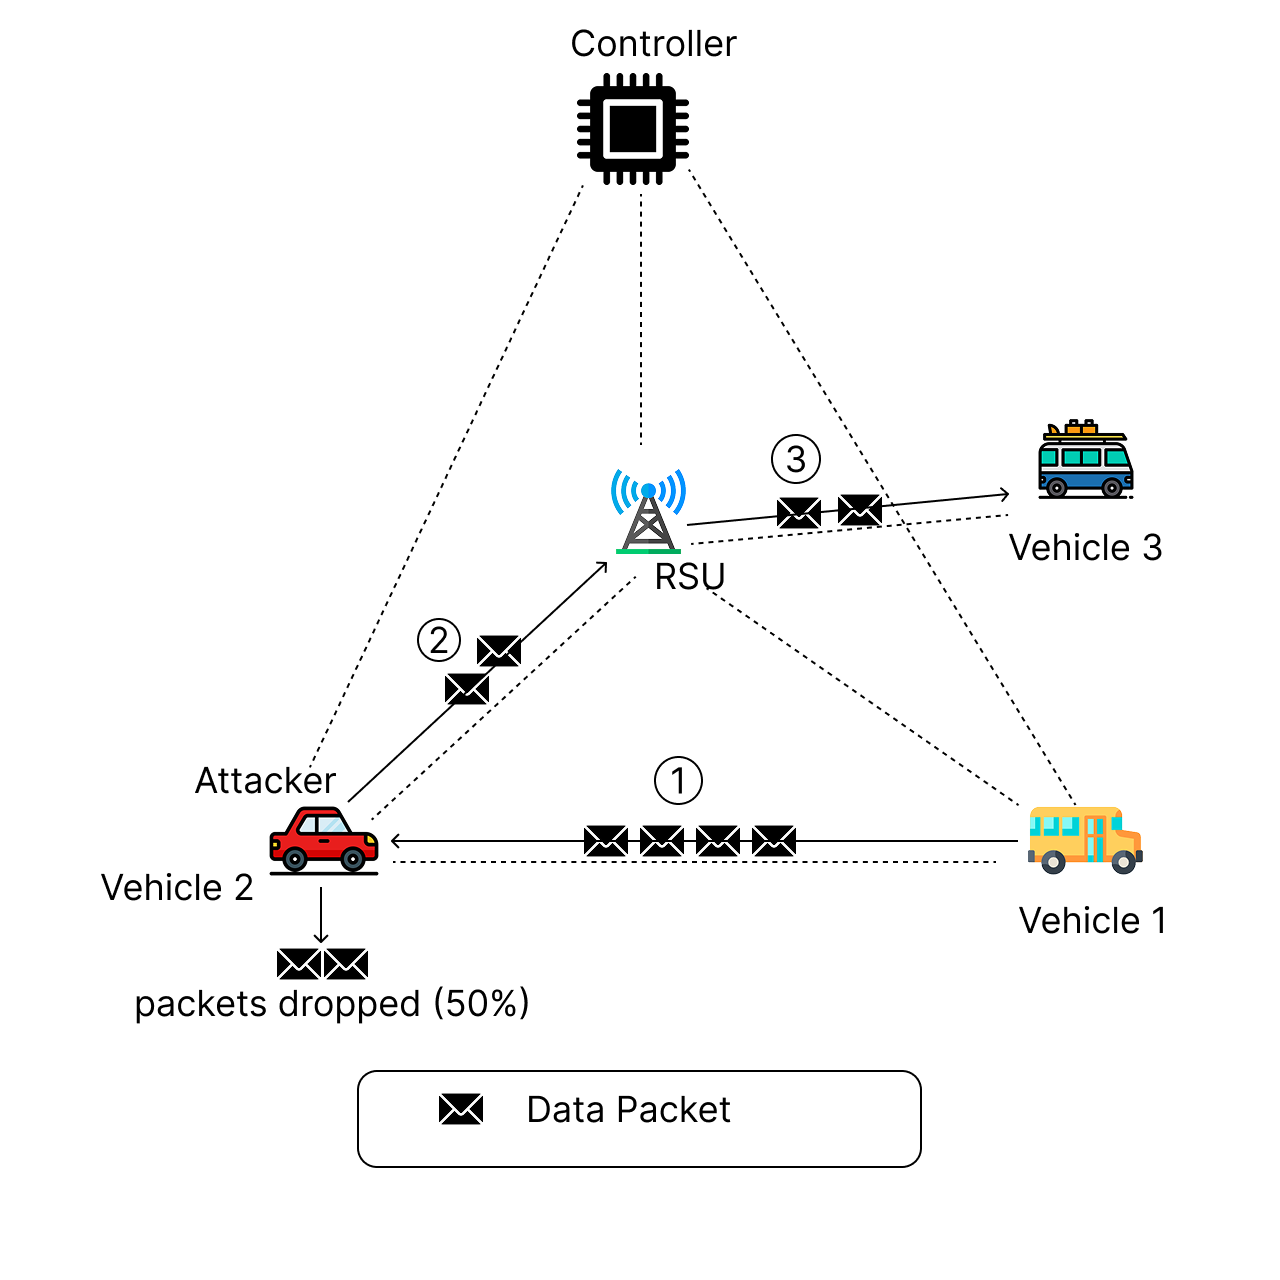
\includegraphics[width=0.7\textwidth,height=0.45\textheight,keepaspectratio]{d_fixed.png}
	\caption{Fixed-rate selective dropping Grey Hole attack in the data plane}
	\label{fig:data-plane-fixed-rate}
\end{figure}

\mypar
Figure \ref{fig:data-plane-fixed-rate} shows a fixed rate selectively dropping grey hole attack of the data plane. According to that figure there are four vehicles and one RSU in that network. In this network, vehicle 2 act as a attacker.

\mypar
As shown in figure \ref{fig:data-plane-fixed-rate} the attacker begins packet dropping by 50\%: data packets arrive from vehicle 1 to vehicle 2 (attacker), which forwards only the remaining 2 packets to the RSU, which then forwards them to vehicle 3.

\mypar
\textbf{Time Based Intermittent Grey Hole Attack in Data Plane}

\mypar
Figure \ref{fig:data-plane-time-normal} and \ref{fig:data-plane-time-malicious} show the time based intermittent grey hole attack scenario in the data plane at two different times. In this scenario there are three vehicles, one RSU, and an SDN controller.

\begin{figure}[H]
	\centering
	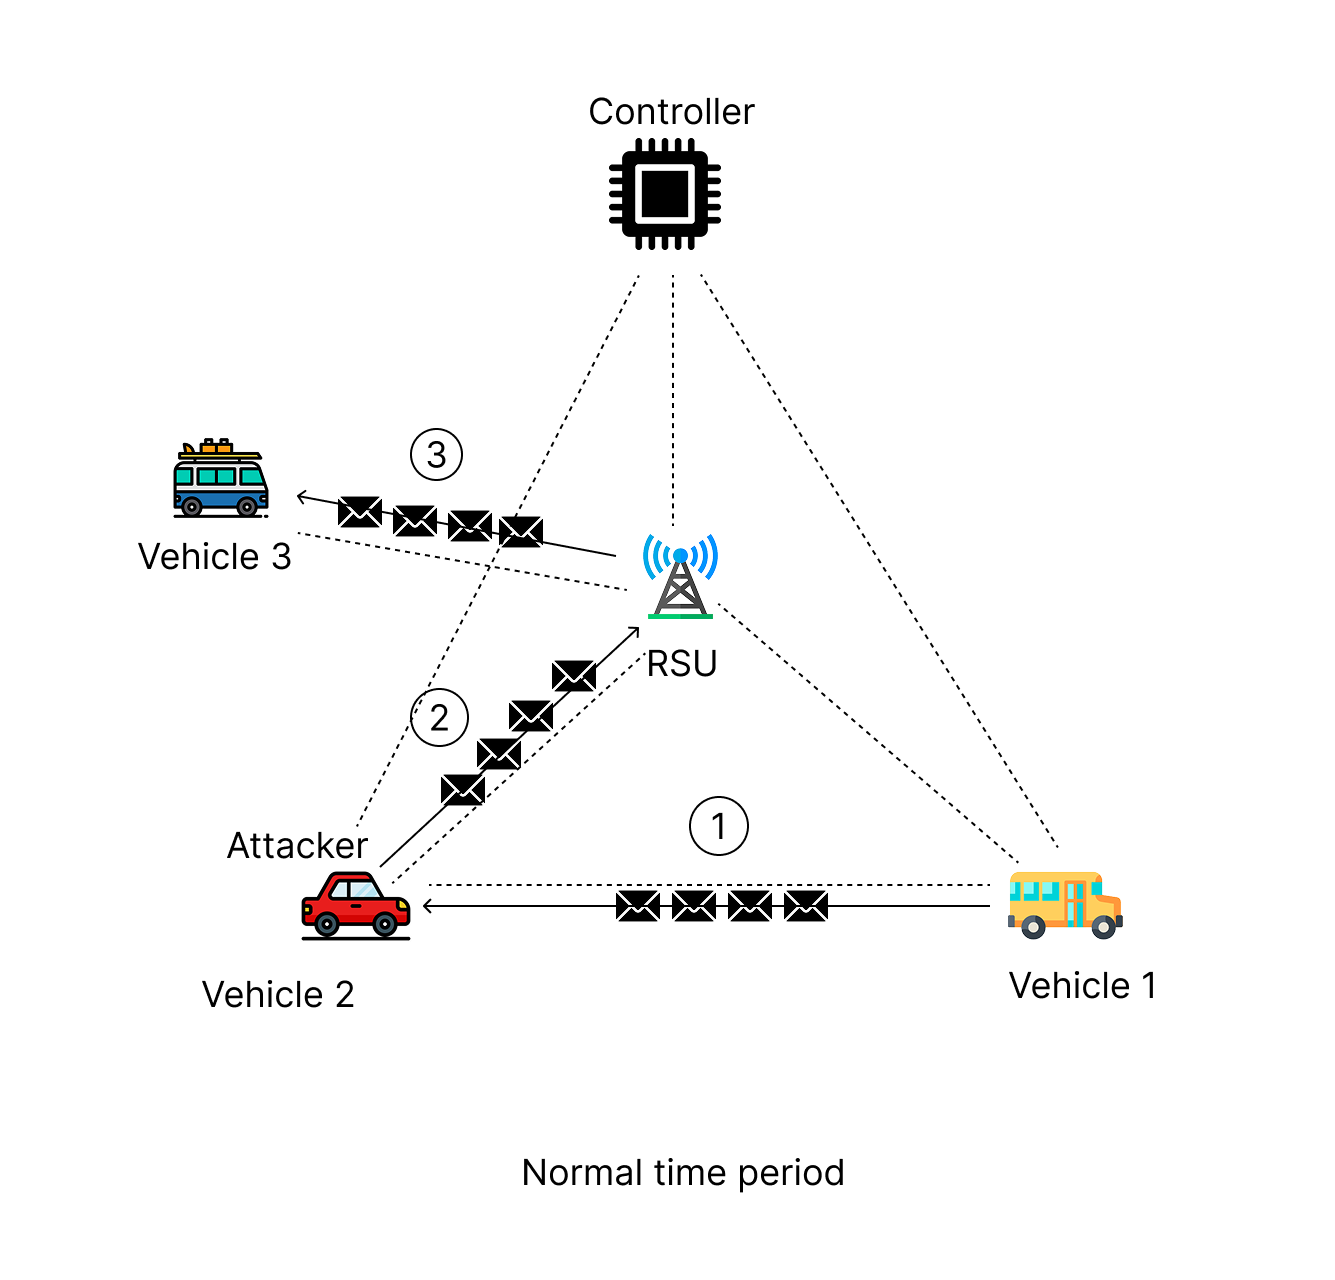
\includegraphics[width=0.8\textwidth,height=0.45\textheight,keepaspectratio]{d_time_normal.png}
	\caption{Normal data-plane behavior at time $t_1$ with no packet dropping}
	\label{fig:data-plane-time-normal}
\end{figure}

\mypar
Figure \ref{fig:data-plane-time-normal} shows the normal behavior of the data plane at time $t = t_1$. All vehicles behave correctly: vehicle V1 sends 4 packets to vehicle 2 (attacker), which forwards all four packets to the RSU, which in turn forwards them to vehicle 3. Communication proceeds normally without any dropping.

\begin{figure}[H]
	\centering
	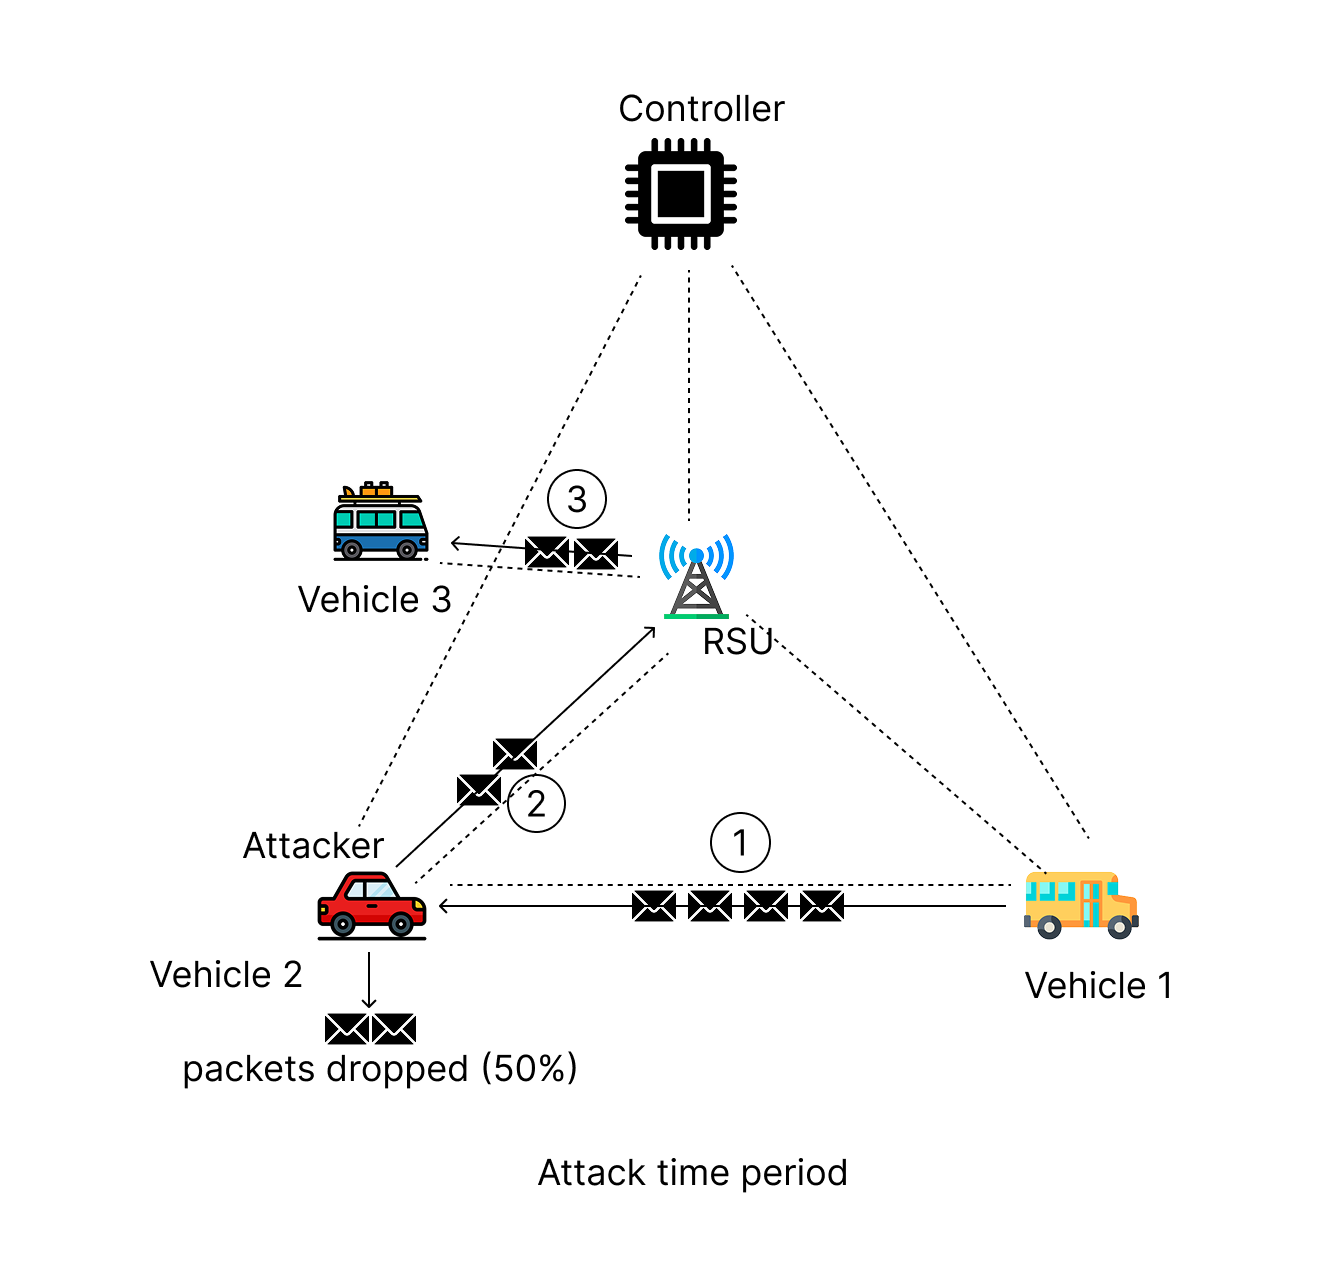
\includegraphics[width=0.8\textwidth,height=0.45\textheight,keepaspectratio]{d_time_malicous.png}
	\caption{Malicious data-plane behavior at time $t_2$ with intermittent packet dropping by V2}
	\label{fig:data-plane-time-malicious}
\end{figure}

\mypar
As shown in figure \ref{fig:data-plane-time-malicious}, at time $t = t_2$, the attacker switches to malicious behaviour: vehicle V1 sends 4 packets to vehicle 2, which drops two packets (50\%) and forwards only the remaining two to the RSU, which forwards them to vehicle 3. The alternation between normal and malicious epochs makes this attack difficult to detect using threshold-based methods.

\mypar
\textbf{Target Specific Intelligent Grey Hole Attack in Data Plane}

\mypar
Figure \ref{fig:d-target} shows the target specific intelligent grey hole attack scenario in the data plane. In this scenario there are four vehicles, one RSU, and a controller. The controller installs flow rules (shown as dashed lines) that vehicle 2 (attacker) selectively enforces.

\mypar
As shown in Figure~\ref{fig:d-target}, vehicle 3 sends three packets to vehicle 2 (attacker), which forwards all three to the RSU without dropping — that path operates correctly according to the flow rule. On a second path, vehicle 1 sends four packets to vehicle 2, which drops 50\% and forwards only two packets to the RSU, which then delivers them to vehicle 4. The attacker thus targets only specific vehicles for dropping, leaving other traffic flows unaffected and making the attack difficult to detect with per-flow aggregates.

\begin{figure}[H]
	\centering
	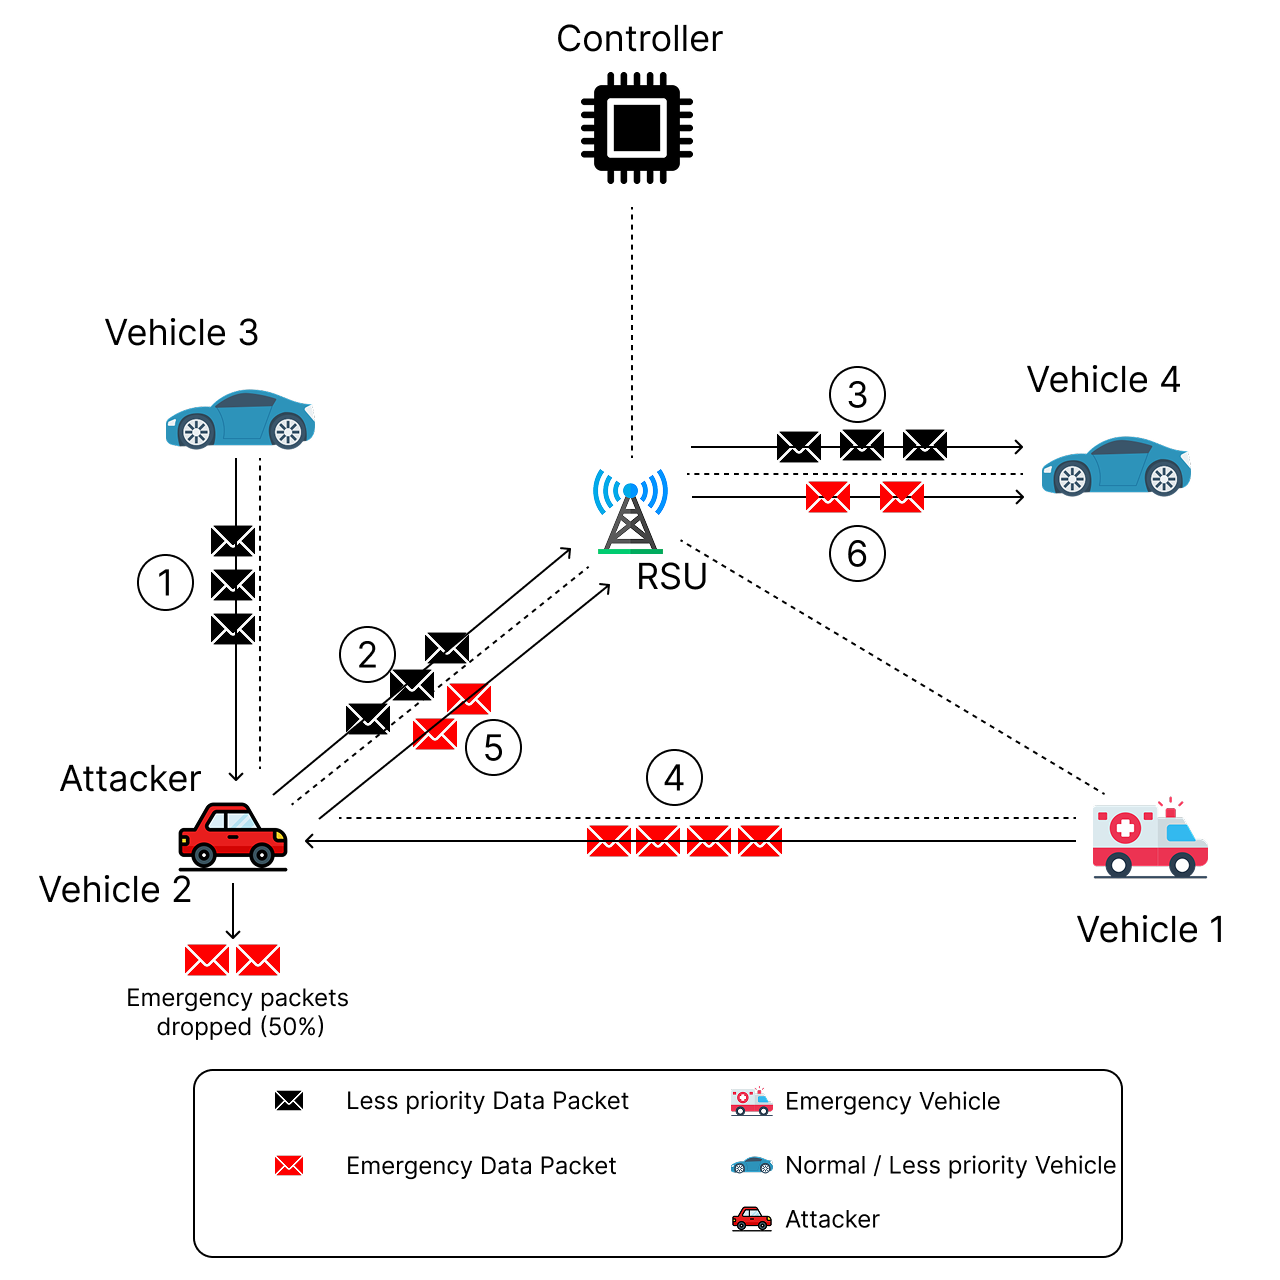
\includegraphics[width=0.8\textwidth,height=0.45\textheight,keepaspectratio]{d_target.png}
	\caption{Target-specific intelligent Grey Hole attack in the data plane}
	\label{fig:d-target}
\end{figure}

\mypar
\subsection{Controller Plane version attack scenarios}

\mypar
\textbf{Fixed Rate Selective Dropping Grey Hole Attack in Controller Plane}

\mypar
Figure~\ref{fig:controller_fixed_rate} show the  fixed rate selectively dropping  grey hole attack scenario in the controller plane. So, in this controller install malicious flow mod rule in the vehicular network act as a attacker.

\mypar
As shown in Figure~\ref{fig:controller_fixed_rate}, first controller install malicious flow mod rule on RSU and the vehicle 2. So, controller configure on the RSU to drop 50\% of all incoming flows and configures on vehicle 2 to drop 60\% of its received packets. 2nd step show vehicel 1 send 5 packets to the vehicel 2 and 3rd step show, vehicle 2 drop three packets according to the malicious configuration. In 4th step send two packets to the vehicle 3 and vehicle forward all two packets to the RSU as a 5th step. Since RSU already configured malicious flow mod rule RSU drop 50\% packets and forward remain packet to the vehicle 4 as 6th step.Since packets are only partially dropped, the communication appears normal, while the overall network performance is gradually degraded also making the attack difficult to detect in like these dynamic vehicular network.

\begin{figure}[H]
	\centering
	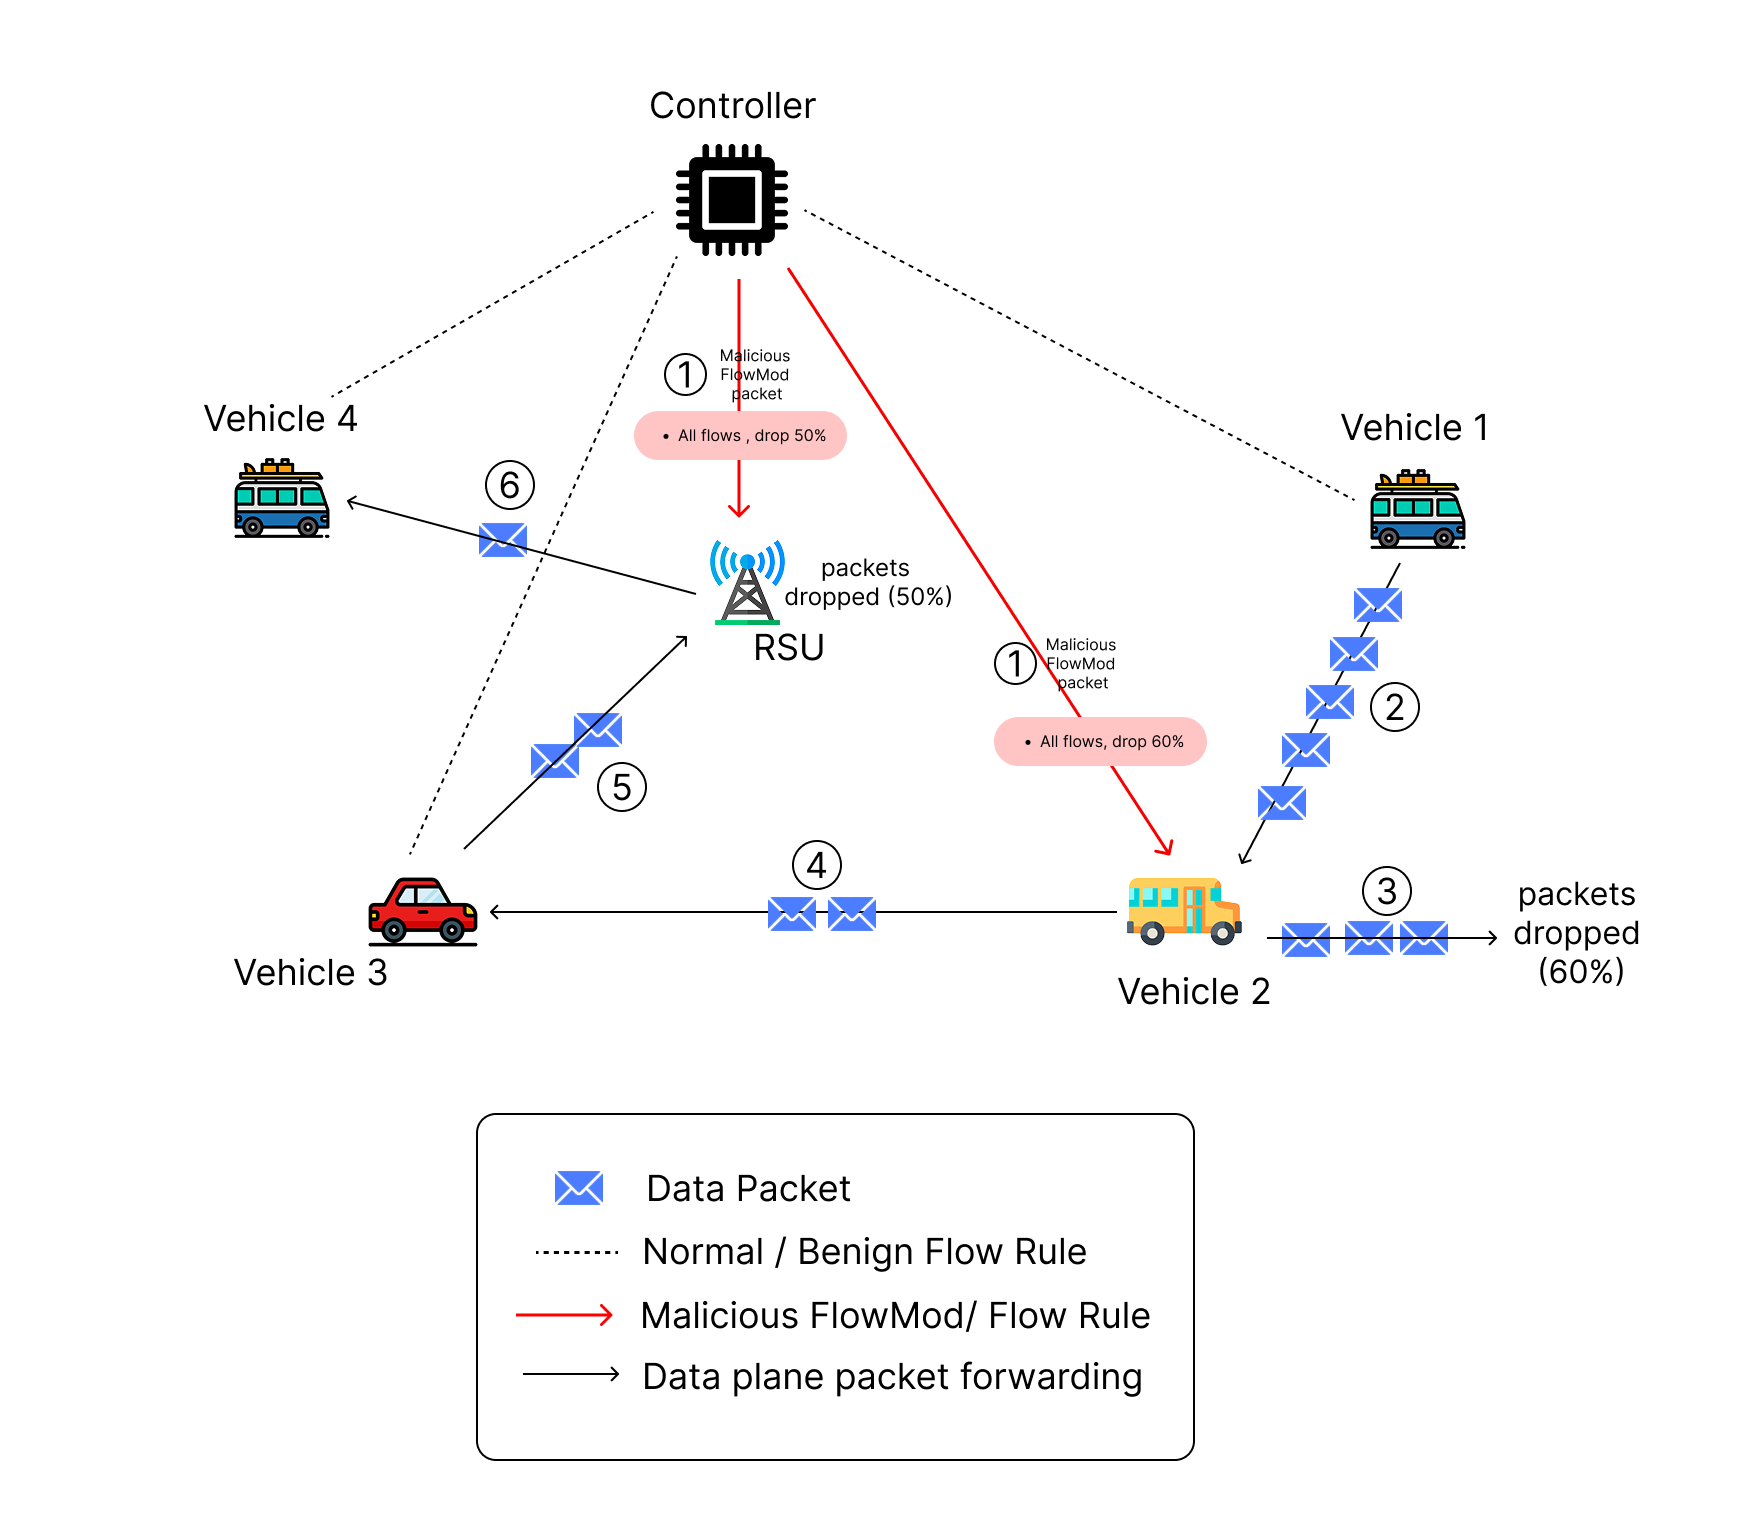
\includegraphics[width=0.8\textwidth,height=0.45\textheight,keepaspectratio]{c_fixed_rate.png}
	\caption{Controller plane fixed rate selective dropping Grey Hole attack}
	\label{fig:controller_fixed_rate}
\end{figure}

\mypar
\textbf{Time Based Intermittent Grey Hole Attack in Controller Plane}

\mypar
Figure  \ref{fig:c_time_normal} and \ref{fig:c_time_malicious} show the time based intermittent gery hole attack scenario in control plane two different times.

\mypar
As shown  \ref{fig:c_time_normal} all steps working without packet dropping according to the flow rule. at time $t = t_1$, the SDN controller behaves normally and does not perform any packet dropping. The controller installs correct flow rules on all vehicles and the RSU.

\begin{figure}[H]
	\centering
	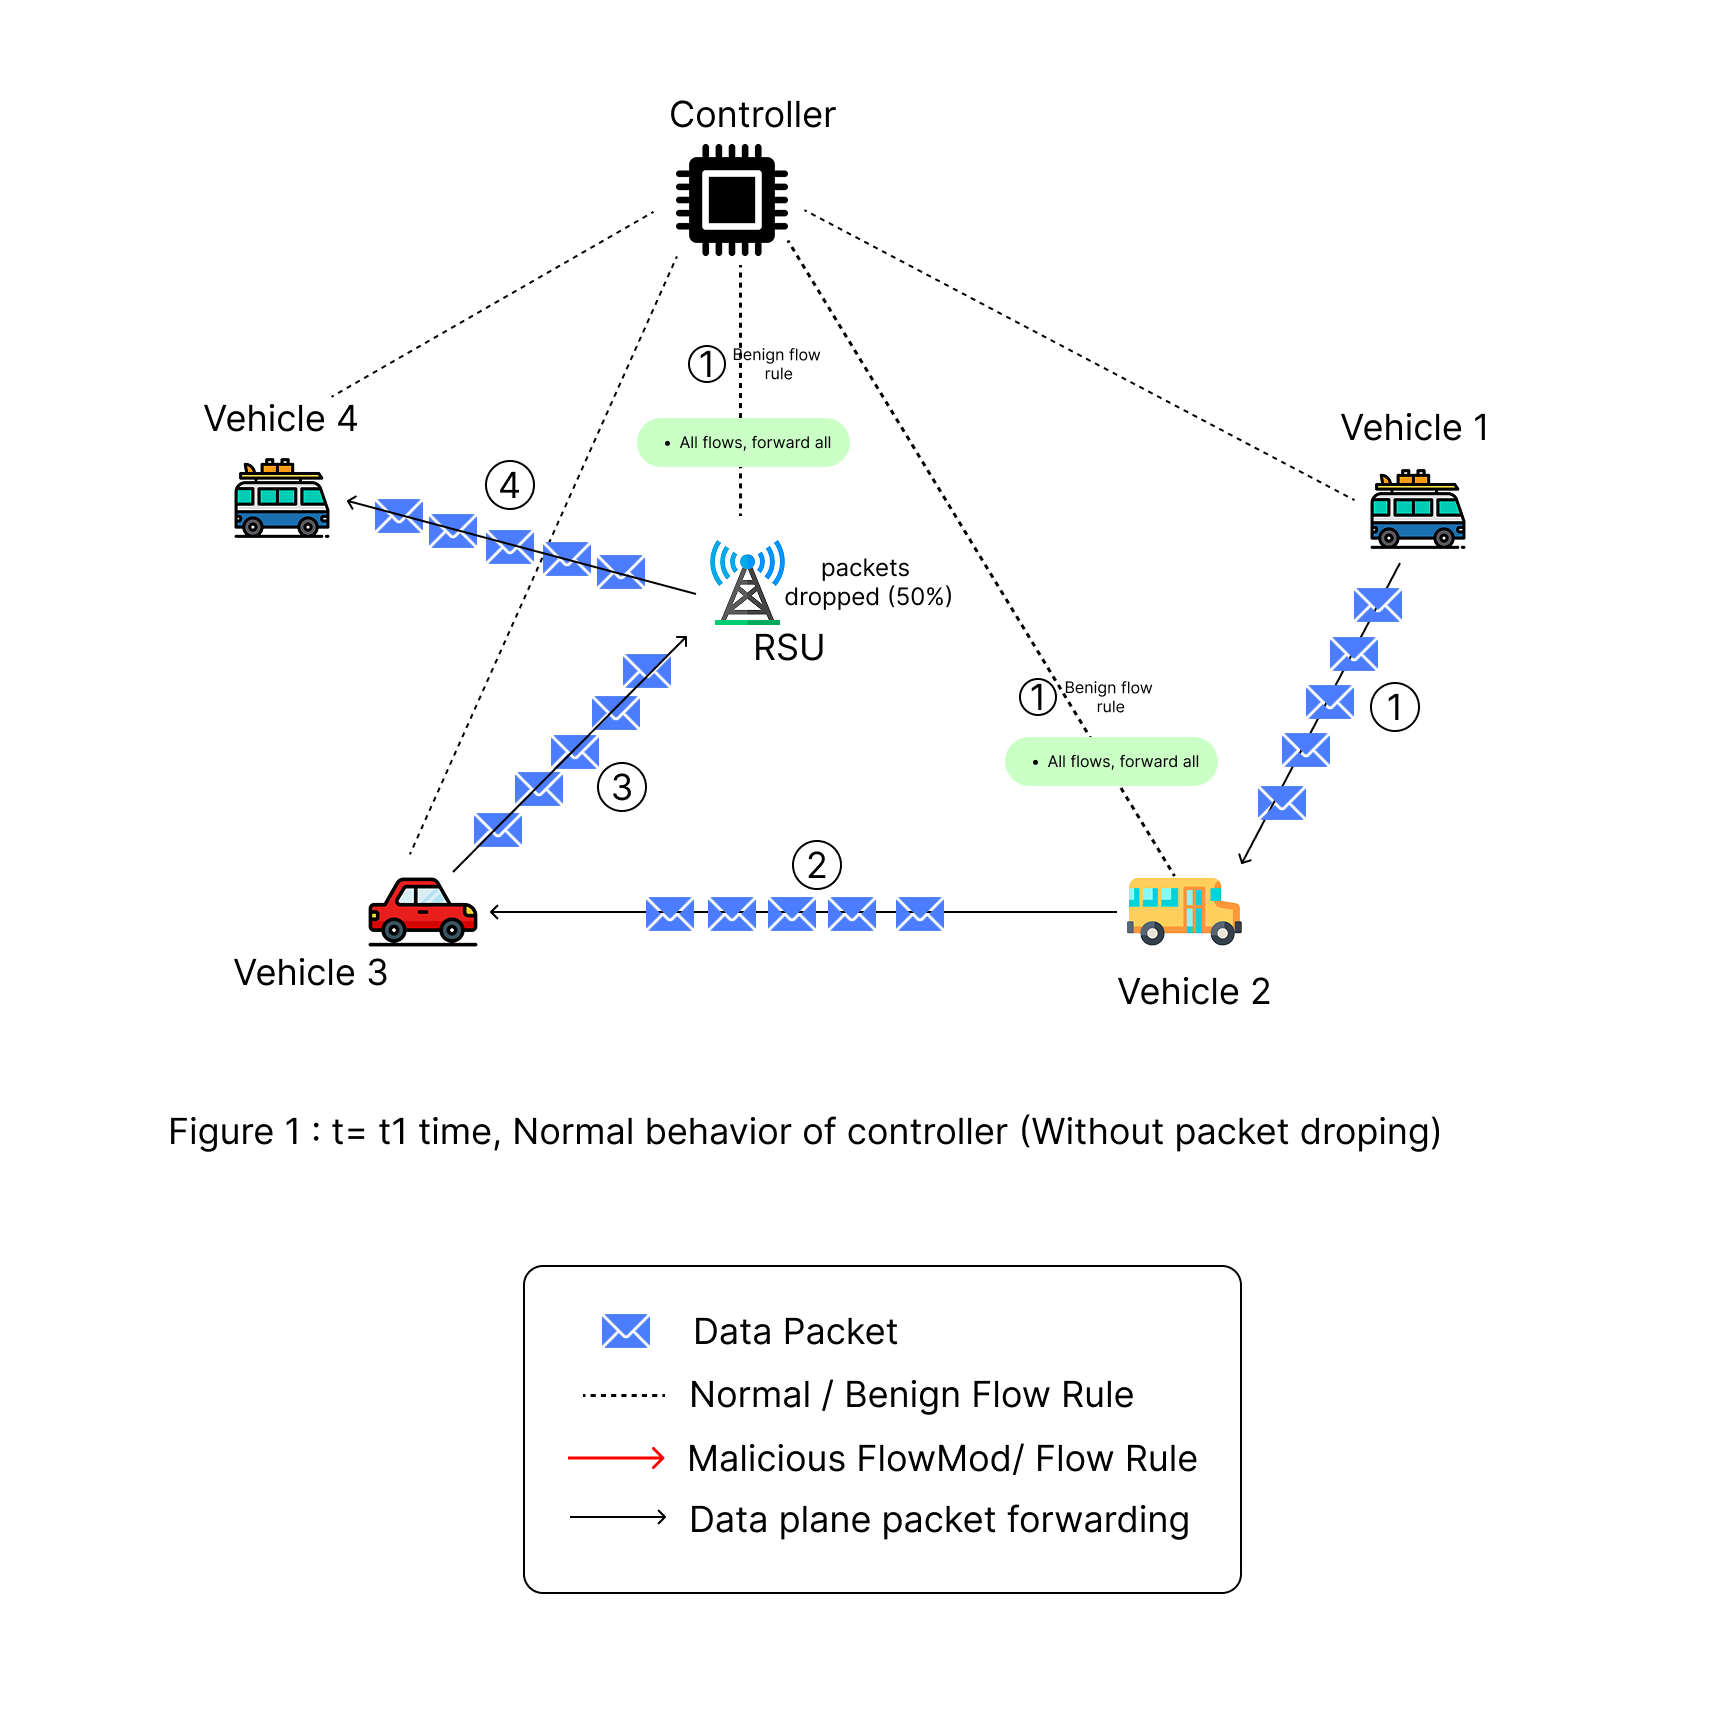
\includegraphics[width=0.85\textwidth,height=0.45\textheight,keepaspectratio]{c_time_normal.png}
	\caption{Normal controller behavior at time $t_1$ with no packet dropping.}
	\label{fig:c_time_normal}
\end{figure}

\mypar
As shown figure~\ref{fig:c_time_malicious} at time $t = t_2$, SDN controller install malicious flow mod rule in the network. So, controller configure on the RSU to drop 50\% all flows and on the vehicle 2 to drop 60\% all flows. Then as the 2nd step vehicle 1 send 5 packets to the vehicle 2 and vehicle 2 drop 60\% packets and forward remain two packets to the vehicle 3 as the 4nd step. In 5th step show vehicle 3 forward that two packets to the RSU. According to the malicious flow mode rule on RSU, RSU drop one packet and forward remain packet to the vehicle 4 as the 6th step.This intermittent behavior allows the controller to hide the attack by switching between normal and malicious operation.

\begin{figure}[H]
	\centering
	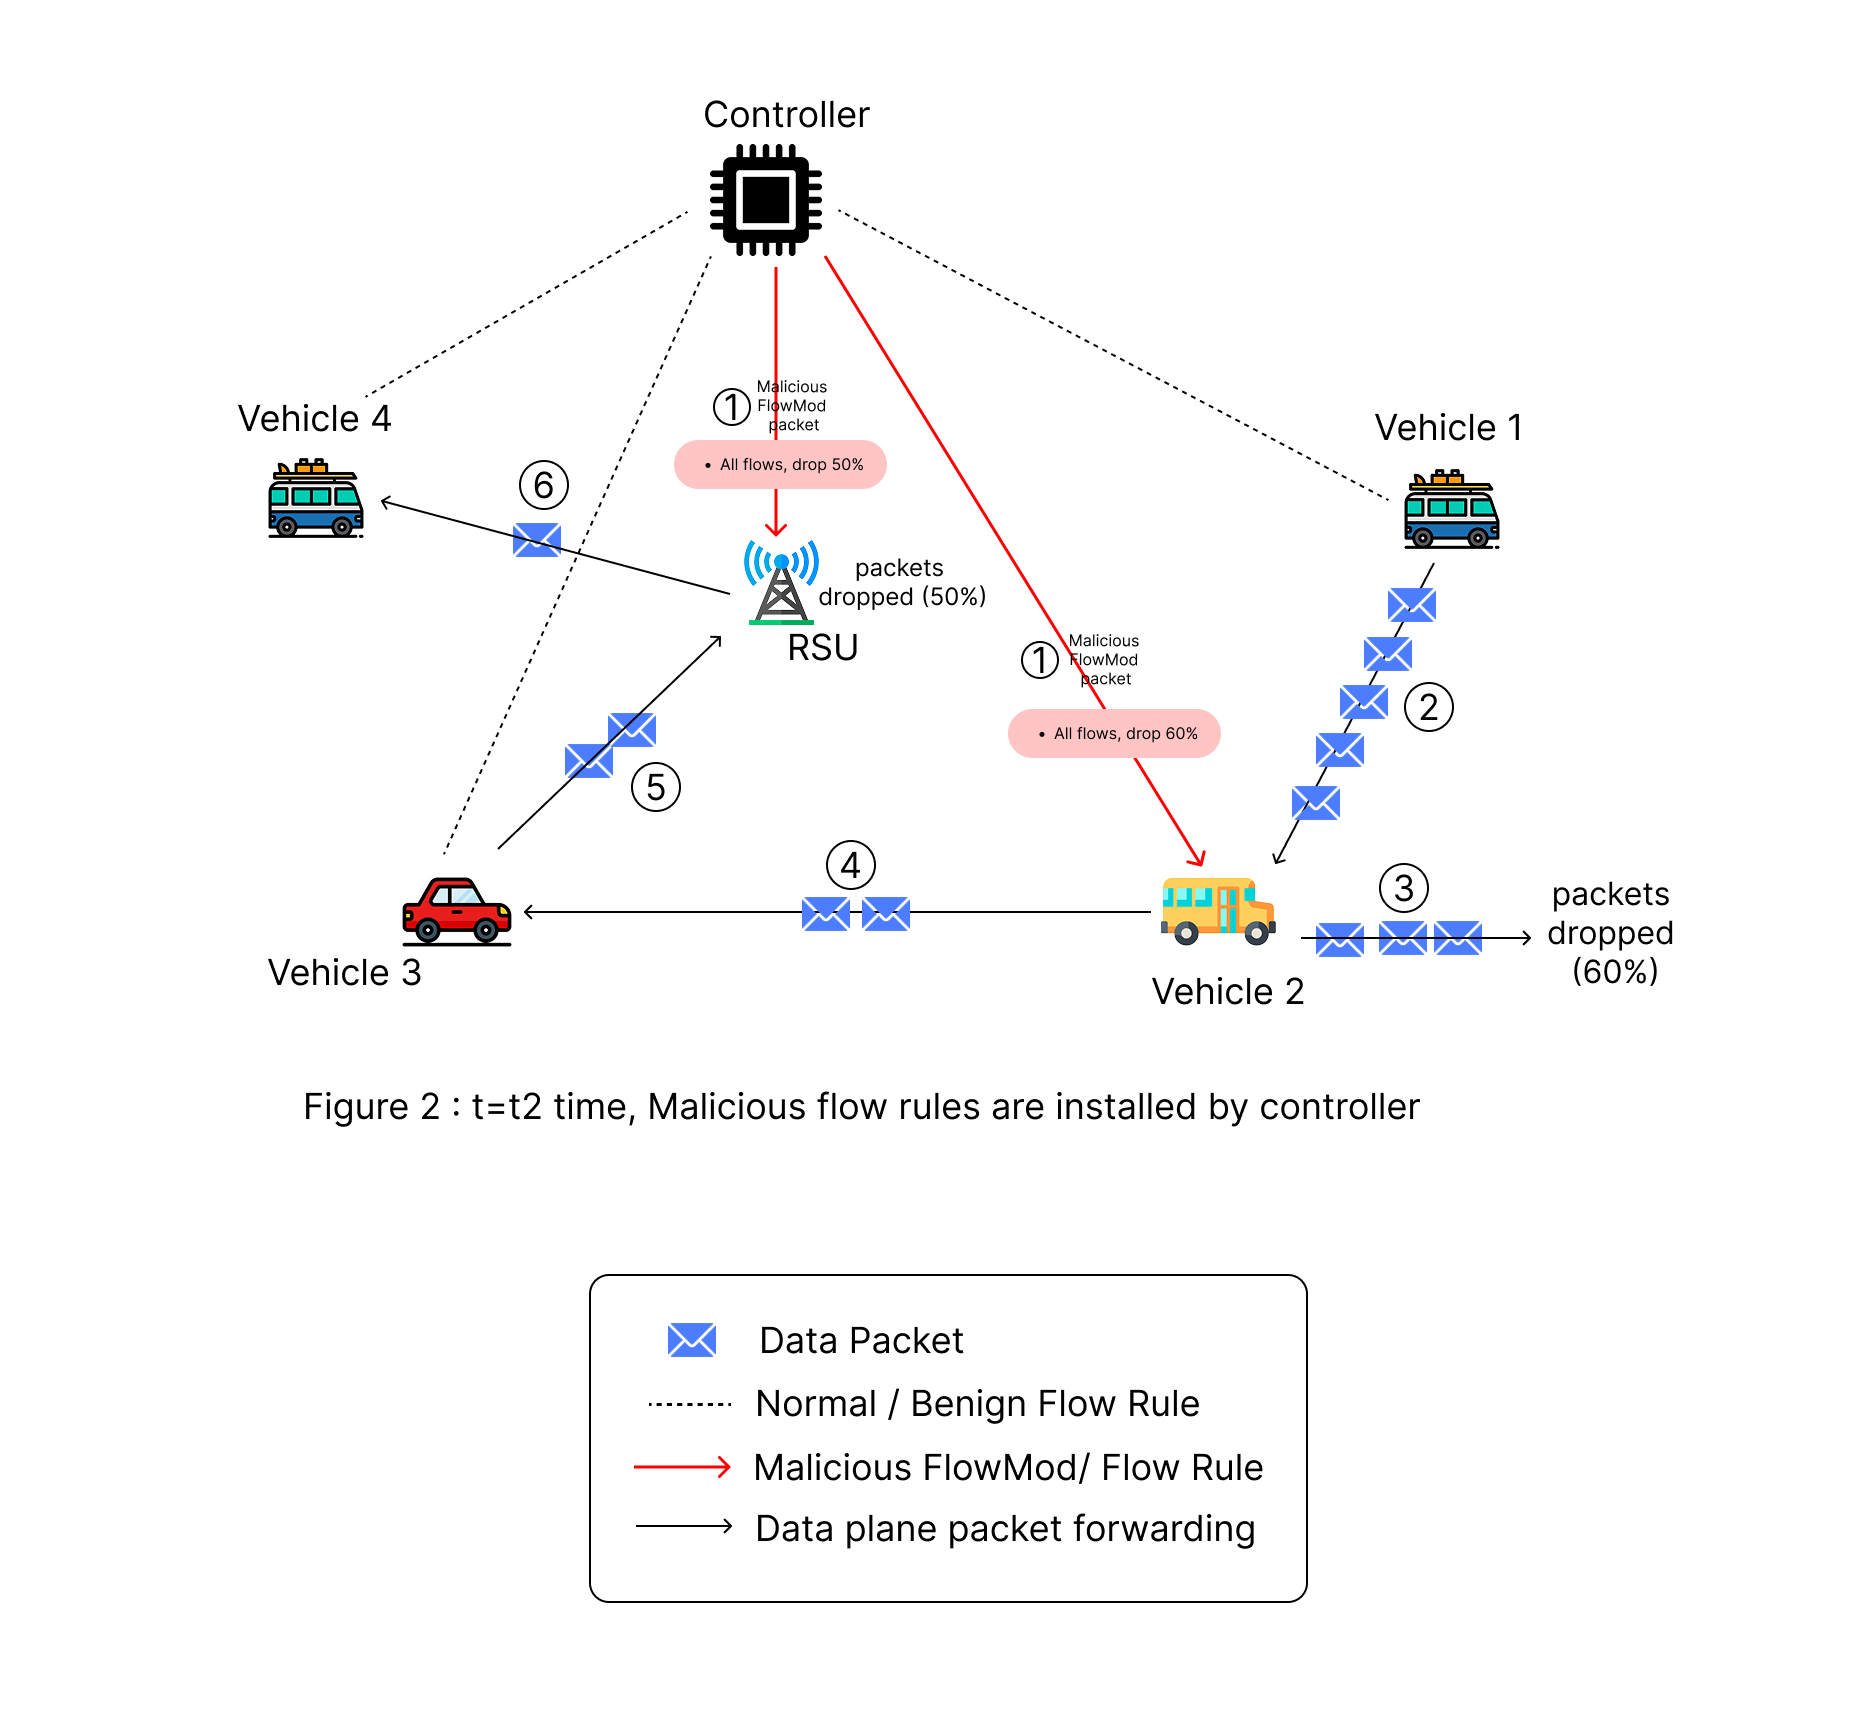
\includegraphics[width=0.85\textwidth,height=0.45\textheight,keepaspectratio]{c_time_malicous.png}
	\caption{Malicious controller behavior at time $t_2$ with selective packet dropping.}
	\label{fig:c_time_malicious}
\end{figure}

\mypar
\textbf{Target Specific Intelligent Grey Hole Attack in Controller Plane}

\mypar
Figure \ref{fig:controller-target-greyhole} shows the target specific intelligent grey hole attack in controller plane. So, in this first controller install flow rule. So, in this figure only install malicious flow mod rule on RSU. So, RSU drop 50\% packets only if source is vehicle 1. All packets came from other sources, forward without any dropping.

\mypar
As shown \ref{fig:controller-target-greyhole}, first step install malicious flow mod rule on RSU. 2nd step shows, vehicle 1 send 4 packets to the RSU and 3 rd step shows, RSU drop two packets since source is vehicle 1. After RSU forward remain 2 packets to the vehicle 4. In step 5 and 6 show the another path packet routing, in that steps there is no any packets dropping since in that path not contain source vehicle 1. In conclusion of this attack scenario, by selectively targeting emergency traffic while forwarding normal traffic, the controller degrades safety critical communication while remaining difficult to detect.

\begin{figure}[H]
	\centering
	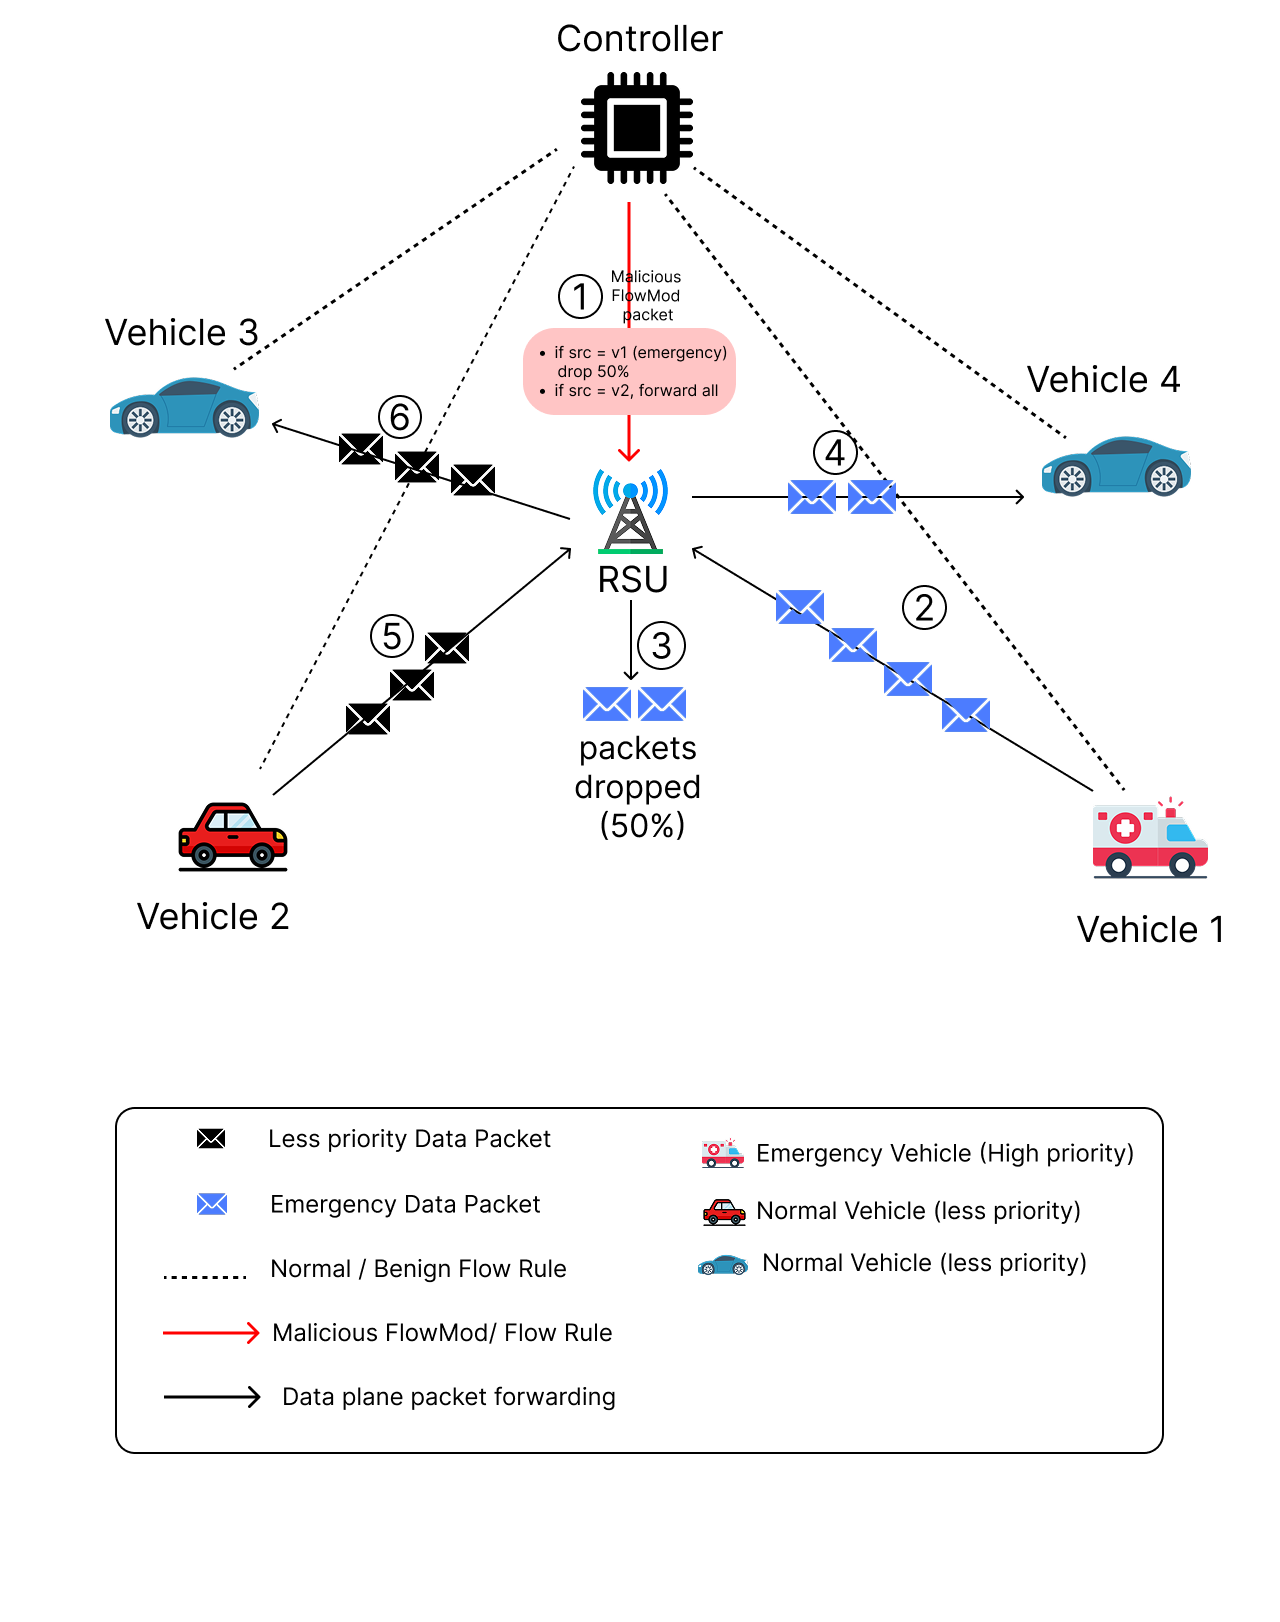
\includegraphics[width=0.85\textwidth,height=0.45\textheight,keepaspectratio]{c_target.png}
	\caption{Target-specific intelligent Grey Hole attack in the controller plane}
	\label{fig:controller-target-greyhole}
\end{figure}

\section{Cryptographic Analysis}
\label{sec:crypto_analysis}

\subsection{Why Cryptography Alone Cannot Mitigate Grey Hole Attacks}

The fundamental property of a grey hole attack is that the attacker is a
\emph{legitimate participant} in the network. It receives authenticated packets
through properly established sessions, holds valid certificates, and produces
correct message authentication codes. Classical cryptographic mechanisms --- HMAC,
ECDSA, TLS --- verify that a packet was not forged or tampered with in transit.
They say nothing about what the receiving node does with the packet after
authentication succeeds.

Formally, let $v_i$ receive packet $p$ authenticated under key $k_i$. Classical
authentication confirms $\texttt{HMAC}(p, k_i) = \texttt{tag}$, establishing
that $p$ arrived intact and from the claimed sender. However, the post-receipt
forwarding decision $\mathbf{1}[v_i \text{ forwards } p]$ is entirely within
$v_i$'s control and is \emph{not constrained} by any authentication mechanism.
A grey hole attacker simply sets this decision to zero for selected packets.
No amount of stronger authentication --- including post-quantum signatures --- changes
this: authentication secures the channel, not the forwarding behaviour of
the channel endpoint.

This is the precise reason why grey hole attacks are harder to detect than
black hole or wormhole attacks: the attacker's traffic is cryptographically
valid at every point it does appear, making statistical anomaly detection the
only viable primary signal.

\mypar
\textbf{Consequence for system design.} Cryptography must be repurposed from
channel authentication to \emph{behaviour attestation}. Instead of proving
that a packet was sent correctly, the cryptographic layer must prove that a
received packet was subsequently forwarded --- or expose the absence of that proof
as a detection signal. This requires a two-phase cryptographic deployment:

\textbf{Phase 1 --- Pre-detection (evidence generation).}
Cryptography generates unforgeable forwarding proofs that serve as input evidence to the detection engine. A grey hole attacker that drops packets \emph{cannot} generate valid proofs for those packets, creating a verifiable discrepancy on the blockchain ledger. This transforms silent dropping into a detectable cryptographic failure without requiring the network to observe the drop directly.

\textbf{Phase 2 --- Post-detection (mitigation enforcement).}
Once the detection engine issues a malicious verdict, cryptography enforces isolation: post-quantum-signed flow modification commands block the attacker's traffic paths; threshold signatures require multi-RSU consensus before blacklisting, preventing single-point false isolation; and group re-keying cryptographically excludes the attacker from future session keys, making continued participation impossible even if the node rejoins under the same identity.

This two-phase design ensures that cryptographic mechanisms contribute to both
detection \emph{and} mitigation, rather than leaving detection entirely to
statistical methods that a sophisticated attacker can evade by calibrating drop
rates below detection thresholds.

\subsection{Selected Cryptographic Techniques by Phase}

The candidate set considered is: \{homomorphic encryption, attribute-based
encryption (ABE), broadcast encryption, homomorphic signatures, ring signatures,
threshold signatures, ZKP, multi-party computation (MPC)\}, with post-quantum
cryptography (PQC) mandatory for quantum-resistance. Techniques are selected
and assigned to phases as follows.

\mypar
\textbf{Phase 1 --- Pre-Detection Evidence Generation}

\textbf{(1) Zero-Knowledge Proofs (ZKP):}
ZKP is the sole technique capable of proving forwarding behaviour without
revealing packet content. Each vehicle $v_i$ commits to its forwarded packet
count via a Pedersen commitment $C_i = g^{n_i^{\text{fwd}}} \cdot h^{r_i}$
(Eq.~\eqref{eq:pedersen}) and generates a proof $\pi_i$
(Eq.~\eqref{eq:zkp_proof}) demonstrating knowledge of a valid opening
consistent with the independently observable blockchain receipt counts. A grey
hole attacker that drops packets cannot produce $\pi_i$ for the dropped batch
because $n_i^{\text{fwd}}$ in its commitment will not match the observable
receipt count on the blockchain --- the discrepancy is the detection signal fed
into the DEBSC gate (Eq.~\eqref{eq:debsc}). ZKP is selected over homomorphic
signatures because it is binding, hiding, and compatible with PQC lattice
constructions, while homomorphic signatures require linear-size proof structures
that scale poorly with batch size.

\textbf{(2) Attribute-Based Encryption (ABE) --- Full mode, target-specific attacks:}
In target-specific attacks, the attacker selectively drops packets from emergency
vehicles while forwarding normal traffic. ABE contributes to detection by
encrypting emergency traffic under the policy \texttt{priority = EMERGENCY}: only
nodes holding valid attribute credentials can decrypt and forward emergency packets.
An attacker without the emergency-traffic credential cannot perform
\emph{content-aware} selective dropping, forcing it to either drop all traffic
(detectable as fixed-rate attack) or forward emergency traffic (attack fails).
ABE is pre-detection because it degrades the attacker's targeting capability,
making its behaviour detectable by the standard PDR signatures S1--S3.

\mypar
\textbf{Phase 2 --- Post-Detection Mitigation Enforcement}

\textbf{(3) Threshold Signatures --- Blacklisting authorisation:}
A $(k,n)$-threshold signature scheme (Eqs.~\eqref{eq:threshold_partial}--\eqref{eq:threshold_verify})
requires $k$ of $n$ RSUs to co-sign the blacklisting decision before the SDN
controller executes isolation. This is critical in high-mobility SDVN where any
single RSU has a short observation window and limited statistical confidence.
Threshold signatures prevent a single compromised or mistaken RSU from unilaterally
isolating a legitimate vehicle. Selected over ring signatures because ring
signatures do not provide individual accountability --- a requirement for auditable
blacklisting in a regulated vehicular network.

\textbf{(4) CRYSTALS-Dilithium --- Flow modification authentication:}
Dilithium (EUF-CMA secure under Module-LWE) authenticates all SDN controller flow
modification commands (Eqs.~\eqref{eq:dilithium_sign}--\eqref{eq:dilithium_verify}).
An OpenFlow switch receiving an isolation command verifies the Dilithium signature
before installing the block rule, preventing a compromised or spoofed controller
from injecting false isolation commands during the re-association window identified
in Section~\ref{sec:mobility_analysis}.

\textbf{(5) CRYSTALS-Kyber (KEM) --- Group re-keying:}
Kyber (IND-CCA2 secure under Module-LWE) encapsulates new group session keys after
isolation (Eqs.~\eqref{eq:kyber_enc}--\eqref{eq:kyber_dec}). The PQC-LKH tree
structure (Section~\ref{sec:pqc_lkh}) reduces re-keying cost from $O(N)$ to
$O(\log N)$ KEM operations. Kyber-512 is used in lightweight mode;
Kyber-768 in full mode.

\mypar
\textbf{Techniques not selected:} Homomorphic encryption and MPC impose
prohibitive computational overhead on vehicle OBU hardware and are excluded.
Broadcast encryption does not address the forwarding proof requirement. Homomorphic
signatures duplicate ZKP functionality at higher proof size and without the
hiding property needed to protect packet content privacy.


\section{Detection Methodology}
\label{sec:detection_methodology}

This section establishes the mathematical foundations for grey hole detection,
modelling packet forwarding behaviour, correcting for mobility-induced loss,
and defining the attack signature conditions used by the detection engine.

\subsection{Packet Forwarding Behaviour Modelling}

To establish a quantitative basis for grey hole detection, we first model the
forwarding behaviour of each vehicle over a sliding observation window. The
\emph{observed packet delivery ratio} of vehicle $v_i$ over a window of $W$
time slots ending at time $t$ is defined as the ratio of packets forwarded to
packets received:

\begin{equation}
\label{eq:pdr}
\text{PDR}_i(t, W) = \frac{\displaystyle\sum_{\tau=t-W}^{t} n_i^{\text{fwd}}(\tau)}
                           {\displaystyle\sum_{\tau=t-W}^{t} n_i^{\text{rx}}(\tau)}
\end{equation}

As shown in Eq.~\eqref{eq:pdr}, the packet delivery ratio $\text{PDR}_i(t, W)$ is the ratio of the total packets forwarded $\sum_\tau n_i^{\text{fwd}}(\tau)$ to the total packets received $\sum_\tau n_i^{\text{rx}}(\tau)$ by vehicle $v_i$ over a sliding window of $W$ time slots ending at time $t$. Here, $n_i^{\text{fwd}}(\tau)$ and $n_i^{\text{rx}}(\tau)$ are the per-slot forwarded and received packet counts respectively. This ratio is the primary forwarding behaviour metric evaluated by all six detection signatures S1--S6.

\noindent where $n_i^{\text{fwd}}(\tau)$ and $n_i^{\text{rx}}(\tau)$ denote
the number of packets forwarded and received by $v_i$ at slot $\tau$.
The \emph{instantaneous drop rate} at a single slot is then:

\begin{equation}
\label{eq:droprate}
\delta_i(t) = 1 - \text{PDR}_i(t, 1)
\end{equation}

As shown in Eq.~\eqref{eq:droprate}, and building on Eq.~\eqref{eq:pdr}, the instantaneous drop rate $\delta_i(t)$ is defined as one minus the single-slot PDR of vehicle $v_i$ at time $t$. A value of $\delta_i(t) = 0$ indicates all received packets were forwarded, while $\delta_i(t) = 1$ indicates all were dropped. This per-slot measure is used in the autocorrelation test of Signature S2 to detect periodic on/off dropping patterns.

Because grey hole attackers exploit the similarity between their behaviour and
natural channel loss, we also track the \emph{variance of PDR} over the window
to separate consistently low forwarding (fixed-rate attack) from fluctuating
forwarding (intermittent attack or legitimate loss):

\begin{equation}
\label{eq:pdr_var}
\sigma^2_i(W) = \frac{1}{W} \sum_{\tau=t-W}^{t}
\!\left(\text{PDR}_i(\tau,1) - \overline{\text{PDR}}_i(W)\right)^2
\end{equation}

As shown in Eq.~\eqref{eq:pdr_var}, the PDR variance $\sigma_i^2(W)$ is the mean squared deviation of the per-slot PDR from the window mean $\overline{\text{PDR}_i}(W)$ over window $W$. Here, $\text{PDR}_i(\tau, 1)$ is the single-slot PDR at slot $\tau$ and $\overline{\text{PDR}_i}(W)$ is the mean PDR over the full window. Low variance combined with a low mean PDR triggers Signature S1 (fixed-rate attack), while high variance suggests either intermittent dropping or legitimate channel loss.

% \noindent where $\overline{\text{PDR}}_i(W)$ is the mean PDR over the window.

\subsection{Mobility-Aware Packet Loss Correction}

In SDVN, RSU handoff events cause transient packet loss that is topologically
expected and must be separated from malicious dropping before any signature
test is applied. We model the \emph{expected handoff-induced loss rate}
$\rho_{ho}(v_i, t)$ as a linear function of vehicle speed $s_i(t)$ normalised
by the RSU coverage radius $R_{\text{RSU}}$:

\begin{equation}
\label{eq:handoff_loss}
\rho_{ho}(v_i, t) = \frac{s_i(t) \cdot \Delta t_{ho}}{R_{\text{RSU}}}
\cdot \rho_{\max}
\end{equation}

As shown in Eq.~\eqref{eq:handoff_loss}, the expected handoff-induced loss rate $\rho_{\text{ho}}(v_i, t)$ is modelled as a linear function of vehicle speed $s_i(t)$. Here, $\Delta t_{\text{ho}}$ is the average duration of an RSU handoff transition, $R_{\text{RSU}}$ is the RSU coverage radius, and $\rho_{\text{max}}$ is the worst-case handoff loss rate calibrated from simulation. The ratio $s_i(t) \cdot \Delta t_{\text{ho}} / R_{\text{RSU}}$ approximates the fraction of time a vehicle spends in a handoff transition, and multiplying by $\rho_{\text{max}}$ yields the expected loss contribution.

\noindent where $\Delta t_{ho}$ is the average handoff transition duration and
$\rho_{\max}$ is the worst-case handoff loss rate calibrated from simulation.
The \emph{mobility-corrected PDR} adds this expected loss back so that the
signature engine operates on behaviour net of topology effects:

\begin{equation}
\label{eq:mobility_pdr}
\widehat{\text{PDR}}_i(t, W) = \text{PDR}_i(t, W) + \rho_{ho}(v_i, t)
\end{equation}

As shown in Eq.~\eqref{eq:mobility_pdr}, the mobility-corrected PDR $\widehat{\text{PDR}}_i(t, W)$ is obtained by adding the expected handoff-induced loss rate $\rho_{\text{ho}}(v_i, t)$ from Eq.~\eqref{eq:handoff_loss} back to the observed PDR from Eq.~\eqref{eq:pdr}. This correction ensures that all six attack signatures S1--S6 are evaluated on forwarding behaviour net of topology-induced effects. Without this correction, a legitimate high-speed vehicle undergoing RSU handoff would exhibit a PDR drop that could incorrectly trigger Signature S1.

\subsection{Attack Signature Conditions}
\label{sec:signatures}

The six formal attack signatures are stated as binary indicator functions
over the mobility-corrected statistics derived above. Each signature is
evaluated independently by the lightweight rule-based detector.

\textbf{Signature S1 (DP-FR).} A node exhibiting a consistently low
mobility-corrected PDR with small variance satisfies the fixed-rate data-plane
signature, since a deliberate constant drop rate produces a stable
low-forwarding region:

\begin{equation}
\label{eq:sig_dpfr}
\mathcal{S}_{\text{DP-FR}}(v_i) =
\mathbf{1}\!\left[\,
\widehat{\text{PDR}}_i(t, W) < \tau_f \;\wedge\;
\sigma^2_i(W) < \varepsilon_f
\,\right]
\end{equation}

As shown signature S1 in Eq.~\eqref{eq:sig_dpfr} fires when two conditions hold simultaneously on the mobility-corrected statistics: the corrected mean PDR $\widehat{\text{PDR}}_i(t, W)$ from Eq.~\eqref{eq:mobility_pdr} falls below threshold $\tau_f$, and the PDR variance $\sigma_i^2(W)$ from Eq.~\eqref{eq:pdr_var} falls below $\varepsilon_f$. Here, $\tau_f$ is the minimum acceptable forwarding ratio and $\varepsilon_f$ is the maximum allowable variance for a steady-state drop pattern. The combination of low mean and low variance distinguishes a deliberate constant-rate dropper from a vehicle experiencing variable legitimate loss.

\textbf{Signature S2 (DP-IT).} An intermittent attacker alternates between
normal and malicious periods, producing a periodic binary pattern in the
instantaneous drop signal. We detect this via the empirical autocorrelation
$R_{m_i}(T) = \frac{1}{W}\sum_\tau m_i(\tau)\,m_i(\tau{-}T)$ of the binary
malicious indicator $m_i(\tau)=\mathbf{1}[\text{PDR}_i(\tau,1)<\tau_{it}]$:

\begin{equation}
\label{eq:sig_dpit}
\mathcal{S}_{\text{DP-IT}}(v_i) =
\mathbf{1}\!\left[\,
\exists\,T^* \in [T_{\min}, T_{\max}] : R_{m_i}(T^*) > \gamma_{it}
\,\right]
\end{equation}

As shown signature S2 in Eq.~\eqref{eq:sig_dpit} detects intermittent dropping by computing the empirical autocorrelation $R_{m_i}(T) = \frac{1}{W}\sum_\tau m_i(\tau) m_i(\tau - T)$ of the binary drop indicator $m_i(\tau) = \mathbf{1}[\text{PDR}_i(\tau, 1) < \tau_{\text{it}}]$. Here, $\tau_{\text{it}}$ is the per-slot drop threshold, $T^*$ is the candidate period, $[T_{\min}, T_{\max}]$ is the expected attack cycle range, and $\gamma_{\text{it}}$ is the autocorrelation significance threshold. The signature fires when a statistically significant periodic component exists, identifying an attacker whose malicious epochs repeat at a fixed cycle.

\textbf{Signature S3 (DP-TS).} A target-specific attacker drops packets
selectively by source, so its per-source PDR distribution deviates
significantly from the uniform baseline expected of a benign forwarder.
We quantify this deviation using the KL-divergence between the empirical
per-source PDR distribution $P_{\text{PDR}_i}^{(s)}$ and the uniform
reference $\mathcal{U}$:

\begin{equation}
\label{eq:sig_dpts}
\mathcal{S}_{\text{DP-TS}}(v_i) =
\mathbf{1}\!\left[\,
D_{\mathrm{KL}}\!\left(P_{\text{PDR}_i}^{(s)} \;\|\; \mathcal{U}\right)
> \tau_{ts}
\,\right]
\end{equation}

As shown signature S3 in Eq.~\eqref{eq:sig_dpts} quantifies selective per-source dropping by computing the KL-divergence $D_{\text{KL}}\!\left(P_{\text{PDR}_i}^{(s)} \| U\right)$ between the empirical per-source PDR distribution $P_{\text{PDR}_i}^{(s)}$ and the uniform reference distribution $U$. Here, $P_{\text{PDR}_i}^{(s)}$ captures how forwarding rates vary across different traffic sources, and $\tau_{\text{ts}}$ is the divergence threshold. A high KL-divergence indicates that vehicle $v_i$ forwards traffic from some sources normally while dropping from others, which is the defining characteristic of a target-specific grey hole attacker.

\textbf{Signature S4 (CP-FR).} In the controller plane, a malicious controller
injects flow rules that unconditionally drop a fixed fraction of all flows.
The signature fires when any installed flow rule carries a drop action with
probability exceeding threshold $\tau_c$:

\begin{equation}
\label{eq:sig_cpfr}
\mathcal{S}_{\text{CP-FR}}(c) =
\mathbf{1}\!\left[\,
\exists\,f \in \mathcal{F}_c(t) :
\mathrm{action}(f) = \texttt{drop} \;\wedge\;
p_{\text{drop}}(f) > \tau_c
\,\right]
\end{equation}

As shown signature S4 in Eq.~\eqref{eq:sig_cpfr} fires when any flow rule $f$ in the active flow table $F_c(t)$ of controller $c$ carries a DROP action with an unconditional drop probability $p_{\text{drop}}(f)$ exceeding threshold $\tau_c$. Here, $F_c(t)$ is the set of all flow rules currently installed by controller $c$, $\text{action}(f)$ is the action field of rule $f$, and $p_{\text{drop}}(f)$ is the associated drop probability. Unlike data-plane signatures, this check operates directly on the flow rule set and does not require historical PDR data.

\textbf{Signature S5 (CP-IT).} An intermittent controller attacker alternates
between benign and malicious flow-rule epochs. Using the same autocorrelation
test applied to the time series of malicious flow-rule counts
$\mathcal{F}_c^{\text{mal}}(t)$, the signature is:

\begin{equation}
\label{eq:sig_cpit}
\mathcal{S}_{\text{CP-IT}}(c) =
\mathbf{1}\!\left[\,
R_{\mathcal{F}_c^{\text{mal}}}(T^*) > \gamma_c \;\wedge\;
\overline{\mathcal{F}_c^{\text{mal}}}(W) > 0
\,\right]
\end{equation}

As shown signature S5 in Eq.~\eqref{eq:sig_cpit} applies the same autocorrelation test as Eq.~\eqref{eq:sig_dpit} to the time series of malicious flow-rule counts $F_c^{\text{mal}}(t)$ recorded in the blockchain log of controller $c$. Here, $R_{F_c^{\text{mal}}}(T^*)$ is the autocorrelation at candidate period $T^*$, $\gamma_c$ is the significance threshold, and $F_c^{\text{mal}}(W) > 0$ confirms at least one malicious rule was observed in the window. The signature detects a compromised controller that alternates between installing benign and malicious flow rules at a fixed period.

\textbf{Signature S6 (CP-TS).} A target-specific controller attack is
distinguished from a fixed-rate attack by the presence of non-wildcard match
fields in the drop rule --- i.e., the drop action is conditioned on a specific
source IP, priority level, or traffic class:

\begin{equation}
\label{eq:sig_cpts}
\mathcal{S}_{\text{CP-TS}}(c) =
\mathbf{1}\!\left[\,
\exists\,f \in \mathcal{F}_c(t) :
\mathrm{action}(f) = \texttt{drop} \;\wedge\;
\mathrm{match}(f) \neq \texttt{WILDCARD}
\,\right]
\end{equation}

As shown, signature S6 in Eq.~\eqref{eq:sig_cpts} fires when any flow rule $f$ installed by controller $c$ carries a DROP action conditioned on a non-wildcard match field, i.e., $\text{match}(f) \neq \text{WILDCARD}$. Here, $F_c(t)$ is the active flow rule set, $\text{action}(f)$ is the rule action, and a non-wildcard match field indicates the drop applies only to a specific source IP, destination, or traffic priority class. This distinguishes a target-specific attack from the fixed-rate case in Eq.~\eqref{eq:sig_cpfr}, where the drop rule applies uniformly to all flows.

\section{Detection and Mitigation Framework}
\label{sec:design}

The proposed framework goes beyond applying existing technologies by
introducing three design-level innovations that address SDVN-specific
constraints not resolvable by straightforward technology deployment.

\subsection{Dual-Evidence Blockchain Smart Contract (DEBSC)}

Naive application of blockchain to vehicular security simply logs node
behaviours as immutable records and relies on a single reputation
threshold to trigger isolation. This design fails in SDVN for two
reasons: (i) mobility causes legitimate PDR volatility that crosses
reputation thresholds, producing false isolations; and (ii) a
sophisticated attacker that is aware of the threshold can calibrate
drop rates just below it while still maintaining effective attack
throughput.

The DEBSC resolves both issues through a dual-evidence gate: isolation
is only authorized when a statistical anomaly (low MATD-corrected
reputation score) AND a cryptographic failure (invalid ZKP forwarding
proof) are detected simultaneously. Formally, from Eq.~\eqref{eq:debsc}:

\begin{equation}
\label{eq:debsc_design}
\mathrm{Isolate}(v_i) = \underbrace{\mathbf{1}\bigl[(1-\mathcal{R}_i) > \theta_R\bigr]}_{\text{Statistical gate}}
\;\wedge\;
\underbrace{\mathbf{1}\bigl[\Pi_{\mathrm{ZKP}}(v_i) = \texttt{FAIL}\bigr]}_{\text{Cryptographic gate}}
\end{equation}

As shown in Eq.~\eqref{eq:debsc_design}, vehicle $v_i$ is isolated only when both conditions are satisfied simultaneously: the reputation deficit $(1 - R_i)$ exceeds threshold $\theta_R$ (statistical gate), and the zero-knowledge proof $\Pi_{\text{ZKP}}(v_i)$ fails (cryptographic gate). Here, $R_i$ is the blockchain reputation score and $\theta_R$ is the isolation threshold. Both gates must fail together to trigger isolation, preventing false positives from either evidence source alone.

The design insight is that a legitimate vehicle with genuine packet loss
(e.g., during RSU handoff) will have a temporarily low reputation but
will still produce valid ZKP forwarding proofs for the packets it did
forward — so only the statistical gate fires and isolation is blocked.
A grey hole attacker that drops packets cannot produce valid proofs for
the dropped packets, so both gates fire and isolation proceeds. This
dual-gating design reduces false isolations to near zero while maintaining
detection sensitivity, a property not achievable by either mechanism alone.

The DEBSC also implements a \emph{graduated response} rather than a
binary isolate/accept decision. Define the \emph{suspicion level}
$\Lambda_i(t)$ as the number of consecutive rounds in which the statistical
gate has fired:

\begin{equation}
\label{eq:suspicion}
\Lambda_i(t) = \sum_{\tau=t-W_s}^{t}
\mathbf{1}\bigl[(1-\mathcal{R}_i(\tau)) > \theta_R\bigr]
\end{equation}

As shown in Eq.~\eqref{eq:suspicion}, the suspicion level $\Lambda_i(t)$ counts the number of consecutive rounds within sliding window $W_s$ in which the statistical gate has fired for vehicle $v_i$. Here, $\theta_R$ is the reputation threshold and $R_i(\tau)$ is the reputation score at round $\tau$. A higher $\Lambda_i(t)$ triggers progressively stricter graduated responses from the smart contract.



The smart contract applies three graduated responses: (1) for
$\Lambda_i < \lambda_1$, rate-limit traffic from $v_i$; (2) for
$\lambda_1 \leq \Lambda_i < \lambda_2$, require ZKP proof verification
for every packet batch; (3) for $\Lambda_i \geq \lambda_2$ and
$\Pi_{\mathrm{ZKP}}(v_i) = \texttt{FAIL}$, trigger full isolation.
This design eliminates the abrupt false-isolation problem of
threshold-based single-evidence systems.

\subsection{Blockchain-Anchored FL Gradient Integrity Verification}

Standard federated learning is vulnerable to model poisoning: a malicious
vehicle submits corrupted gradient updates to degrade the global detection
model. Existing defences (e.g., robust aggregation, anomaly filtering on
gradient norms) are computationally intensive and require a trusted
aggregator — which does not exist in a decentralised SDVN.

The proposed design anchors each gradient update to the blockchain
\emph{before} the aggregation round. Each vehicle $v_i$ submits a
commitment $\mathcal{C}_i = \texttt{Hash}(\Delta\mathbf{w}_i \| t \| \mathrm{id}_i)$
to the blockchain at the start of the round, and transmits
$\Delta\mathbf{w}_i$ to the aggregator. The aggregator verifies:

\begin{equation}
\label{eq:gradient_commit}
\texttt{Valid}_i = \mathbf{1}\bigl[
\texttt{Hash}(\Delta\mathbf{w}_i \| t \| \mathrm{id}_i) =
\mathcal{C}_i^{\mathrm{BC}}
\bigr]
\end{equation}

As shown in Eq.~\eqref{eq:eq:gradient_commit}, a gradient update from vehicle $v_i$ is accepted only if the hash of the received gradient $\Delta w_i$ matches the pre-committed hash $C_i^{\text{BC}}$ stored on the blockchain. Here, $\Delta w_i$ is the local model update, $t$ is the round timestamp, and $id_i$ is the vehicle identifier. Any tampered or poisoned gradient will produce a hash mismatch and is rejected before aggregation.

\noindent where $\mathcal{C}_i^{\mathrm{BC}}$ is the commitment retrieved
from the blockchain. Only verified updates enter the FedAvg aggregation
(Eq.~\eqref{eq:fedavg}). The design insight is that a malicious vehicle
cannot retroactively alter its committed gradient — the blockchain's
immutability prevents it. Unlike norm-based filtering, this approach
incurs no gradient computation overhead and does not require a trusted
aggregator, making it suitable for the decentralised SDVN architecture.
Furthermore, the blockchain commitment serves as an auditable provenance
record: if a model degradation is detected post-deployment, the specific
round and vehicle responsible can be traced without violating privacy,
since only hashes are stored on-chain.

\subsection{Edge-LLM Architecture for Real-Time Grey Hole Detection}

Deploying a full LLM on resource-constrained vehicle OBUs is infeasible.
The naive solution — deploying the LLM only on the cloud — introduces
unacceptable latency for real-time safety-critical decisions. Motivated
by the edge-cloud design of MistralBSM~\cite{hamhoum2024mistralbsm},
the proposed framework employs a two-tier LLM deployment:

\textbf{Tier 1 (Edge LLM at RSU):} A quantised, fine-tuned lightweight
LLM (e.g., a 4-bit quantised Mistral-7B or BERT-based model) processes
short blockchain log windows $\mathbf{x}_i^{(t)}$ of length $n_e$ at the
RSU in real time. It produces a binary preliminary verdict
$\hat{y}_i^{\mathrm{edge}} \in \{0,1\}$.

\textbf{Tier 2 (Cloud LLM):} For cases where the edge LLM uncertainty
exceeds threshold $\varepsilon_u$, a full-size LLM processes a longer
historical window of length $n_c \gg n_e$ for a definitive verdict.

The routing decision is:

\begin{equation}
\label{eq:llm_routing}
\text{Use Tier 2} =
\mathbf{1}\bigl[
\max_c \,\mathrm{softmax}(\mathrm{LLM}_{\mathrm{edge}}(\mathbf{x}_i))_c < \varepsilon_u
\bigr]
\end{equation}

As shown in Eq.~\eqref{eq:llm_routing}, the routing condition for the two-tier LLM is defined such that if the maximum softmax confidence of the edge LLM over all classes $c$ falls below uncertainty threshold $\varepsilon_u$, the input $x_i$ is escalated to the cloud-tier LLM for deeper analysis. Here, $\text{LLM}_{\text{edge}}(x_i)$ is the edge model output logit vector and $\varepsilon_u$ is the confidence threshold tuned on the validation set.



The final threat score $\mathcal{Q}_i(t)$ (Eq.~\eqref{eq:llm_score}) is
taken from whichever tier produces the verdict. This design reduces average
inference latency to $\bar{L}_{\mathrm{edge}}$ ms for the majority of cases
(high-confidence edge decisions), while reserving the full cloud LLM for
ambiguous borderline cases — a latency-accuracy trade-off not achieved by
either single-tier deployment. The window size $n_e$ is a design parameter
tuned jointly with $\varepsilon_u$ on the validation split to balance
latency and accuracy.

\subsection{Mobility-Aware Trust Scoring and Blockchain Reputation}

Trust accumulation in high-mobility environments must account for the fact that
short RSU dwell times yield statistically insufficient observations. We adopt a
Bayesian Beta-distribution trust model in which forwarding successes and failures
update the posterior mean, giving the \emph{instantaneous trust score}:

\begin{equation}
\label{eq:trust_update}
\mathcal{T}_i(t) = \frac{\alpha + n_i^{\text{fwd}}(t)}
                         {\alpha + n_i^{\text{fwd}}(t)
                          + \beta + n_i^{\text{drop}}(t)}
\end{equation}

As shown in Eq.~\eqref{eq:trust_update}, the instantaneous trust score $T_i(t)$ models forwarding behaviour as a Beta distribution. Here, $\alpha$ and $\beta$ are Beta prior parameters representing initial trust assumptions, $n_i^{\text{fwd}}(t)$ is the number of packets forwarded, and $n_i^{\text{drop}}(t) = n_i^{\text{rx}}(t) - n_i^{\text{fwd}}(t)$ is the number of packets dropped. More forwarding increases $T_i(t)$ toward 1; more dropping decreases it toward 0.

\noindent where $\alpha$ and $\beta$ are Beta prior parameters and
$n_i^{\text{drop}}(t) = n_i^{\text{rx}}(t) - n_i^{\text{fwd}}(t)$.
A high-speed vehicle accumulates few observations per RSU segment, so blindly
trusting this score risks false isolation. The \emph{Mobility-Aware Trust
Decay (MATD)} applies an exponential penalty proportional to current speed,
reducing the effective trust contribution of high-speed vehicles for which
the observation basis is shallow:

\begin{equation}
\label{eq:matd}
\mathcal{T}_i^{\text{mob}}(t) = \mathcal{T}_i(t) \cdot
e^{-\lambda_s\, s_i(t)\, \Delta t}
\end{equation}

As shown in Eq.~\eqref{eq:matd}, the mobility-corrected trust score $T_i^{\text{mob}}(t)$ is obtained by applying an exponential penalty to the raw trust score $T_i(t)$. Here, $\lambda_s > 0$ is the mobility decay coefficient calibrated to the RSU coverage radius and vehicle density, $s_i(t)$ is the current speed of vehicle $v_i$, and $\Delta t$ is the observation slot duration. Faster vehicles receive a lower trust weight since fewer forwarding observations are available during short RSU dwell times.

\noindent where $\lambda_s > 0$ is the mobility decay coefficient tuned
to the RSU coverage radius and vehicle density. The \emph{blockchain reputation
score} then aggregates MATD-corrected trust over all historical RSU interactions
$\mathcal{H}_i$ stored in the immutable ledger, providing a long-term behavioural
baseline immune to short-term manipulation:

\begin{equation}
\label{eq:reputation}
\mathcal{R}_i(t) = \frac{1}{|\mathcal{H}_i|}
\sum_{h \in \mathcal{H}_i} \mathcal{T}_i^{\text{mob}}(h)
\end{equation}

As shown in Eq.~\eqref{eq:reputation}, the long-term reputation score $R_i(t)$ is the mean of all MATD-corrected trust scores $T_i^{\text{mob}}(h)$ accumulated over the historical RSU interaction set $\mathcal{H}_i$ stored on the immutable blockchain ledger. Here, $|\mathcal{H}_i|$ is the total number of historical interactions. Since the ledger is append-only, $R_i(t)$ cannot be reset by short-term honest behaviour.

To prevent a single corrupted evidence source from triggering false isolation,
the \emph{Dual-Evidence Blockchain Smart Contract (DEBSC)} requires both the
statistical reputation score and the cryptographic forwarding proof to fail
simultaneously before an isolation command is authorised:

\begin{equation}
\label{eq:debsc}
\mathrm{Isolate}(v_i) = \mathbf{1}\!\left[\,
\bigl(1 - \mathcal{R}_i(t)\bigr) > \theta_R \;\wedge\;
\Pi_{\mathrm{ZKP}}(v_i, t) = \texttt{FAIL}
\,\right]
\end{equation}

As shown in Eq.~\eqref{eq:debsc}, the dual-evidence isolation condition authorizes isolation of vehicle $v_i$ only when two independent conditions hold simultaneously: the reputation deficit $(1 - R_i(t))$ exceeds threshold $\theta_R$, and the ZKP forwarding proof $\Pi_{\text{ZKP}}(v_i, t)$ returns FAIL. Here, $R_i(t)$ is the blockchain reputation score from Eq.~\eqref{eq:reputation} and $\theta_R$ is the pre-configured isolation threshold. A legitimate vehicle experiencing handoff-induced packet loss will retain valid ZKP proofs and will not satisfy the cryptographic gate, preventing false isolation.

\subsection{Federated Learning with Blockchain-Verified Gradient Integrity}

Each vehicle $v_i$ trains a local detection model $\mathbf{w}_i$ by minimising
the cross-entropy loss over its local dataset $\mathcal{D}_i$ of labelled
forwarding-log sequences:

\begin{equation}
\label{eq:local_loss}
\mathcal{L}_i(\mathbf{w}) = \frac{1}{|\mathcal{D}_i|}
\sum_{(\mathbf{x},y)\in\mathcal{D}_i}
\ell\!\left(f(\mathbf{x};\mathbf{w}),\, y\right)
\end{equation}

As shown in Eq.~\eqref{eq:local_loss}, each vehicle $v_i$ trains its local detection model by minimizing the cross-entropy loss $\mathcal{L}_i(w)$ over its local dataset $D_i$ of labelled forwarding-log sequences. Here, $w$ is the model weight vector, $x$ is an input forwarding-log feature vector, $y$ is the corresponding ground-truth label, $f(x; w)$ is the model prediction, and $\ell(\cdot)$ is the cross-entropy loss function. This training is performed locally without sharing raw traffic data.

The global model is updated each round $r$ via weighted averaging, where
weights are proportional to local dataset size to account for heterogeneous
vehicular observation volumes:

\begin{equation}
\label{eq:fedavg}
\mathbf{w}^{(r+1)} =
\sum_{i \in \mathcal{A}} \frac{|\mathcal{D}_i|}{|\mathcal{D}_{\mathcal{A}}|}
\mathbf{w}_i^{(r)}
\end{equation}

As shown in Eq.~\eqref{eq:fedavg}, the new global model $w^{(r+1)}$ is computed as a dataset-size-weighted average of the accepted local models $w_i^{(r)}$. Here, $\mathcal{A}$ is the set of accepted vehicles whose gradients passed the blockchain integrity check in Eq.~\eqref{eq:gradient_verify}, $|D_i|$ is the local dataset size of vehicle $v_i$, and $|D_\mathcal{A}| = \sum_{i \in \mathcal{A}} |D_i|$ is the total accepted data volume. Weighting by dataset size reduces the influence of vehicles with sparse observations.

\noindent where $\mathcal{A}$ is the set of accepted vehicles and
$|\mathcal{D}_{\mathcal{A}}| = \sum_{i\in\mathcal{A}}|\mathcal{D}_i|$.
A malicious vehicle can poison the global model by submitting corrupted
gradient updates. To prevent this, each gradient update is hash-committed
to the blockchain before the aggregation round; the aggregator accepts an
update only if its on-chain hash matches the received gradient:

\begin{equation}
\label{eq:gradient_verify}
\mathrm{Accept}(\Delta\mathbf{w}_i) =
\mathbf{1}\!\left[\,
\mathcal{H}_{\mathrm{BC}}(\Delta\mathbf{w}_i) =
\mathtt{Hash}(\Delta\mathbf{w}_i)
\,\right]
\end{equation}

As shown in Eq.~\eqref{eq:gradient_verify}, a local gradient update $\Delta w_i$ is accepted into aggregation only if the hash of the received gradient matches the on-chain commitment $H^{\text{BC}}(\Delta w_i)$ pre-submitted by vehicle $v_i$ before the aggregation round. Here, $\text{Hash}(\Delta w_i)$ is the locally computed hash and $H^{\text{BC}}(\Delta w_i)$ is the hash retrieved from the blockchain. A mismatch indicates tampering or gradient poisoning, and the update is discarded.

\subsection{LLM-Based Semantic Threat Scoring and Fusion}

In the full detection mode, the LLM processes tokenised blockchain forwarding
logs $\mathbf{x}_i^{(t)}$ as a sequence classification task. The threat score
is the softmax probability assigned to the malicious class by the LLM with
parameters $\boldsymbol{\theta}$:

\begin{equation}
\label{eq:llm_score}
\mathcal{Q}_i(t) =
\mathrm{softmax}\!\Bigl(
\mathrm{LLM}\!\left(\mathbf{x}_i^{(t)};\boldsymbol{\theta}\right)
\Bigr)_{\!\mathrm{malicious}}
\end{equation}

As shown in Eq.~\eqref{eq:llm_score}, the LLM-based threat score $Q_i(t)$ is the softmax probability assigned to the malicious class by the fine-tuned LLM with parameters $\theta$. Here, $x_i^{(t)}$ is the tokenized blockchain forwarding log of vehicle $v_i$ at time $t$, and the softmax is evaluated over all output classes with the malicious class probability extracted. A higher $Q_i(t)$ indicates greater likelihood of grey hole behaviour as inferred from the temporal log sequence.

Because no single evidence source is individually sufficient for reliable
detection under all six attack variants, the final detection decision fuses
the rule-based aggregate signature score, the LLM semantic score, and the
blockchain reputation deficit through a learned linear combination:

\begin{equation}
\label{eq:fusion}
\hat{y}_i(t) = \mathbf{1}\!\left[\,
\mu_1\,\mathcal{S}_{\mathrm{total}}(v_i)
+ \mu_2\,\mathcal{Q}_i(t)
+ \mu_3\,\bigl(1 - \mathcal{R}_i(t)\bigr)
> \theta_{\mathrm{det}}
\,\right]
\end{equation}

As shown in Eq.~\eqref{eq:fusion}, the final binary detection verdict $\hat{y}_i(t)$ is produced by combining three evidence streams using learned weights $\mu_1, \mu_2, \mu_3$ subject to $\mu_1 + \mu_2 + \mu_3 = 1$. Here, $S_{\text{total}}(v_i) = \max_k S_k(v_i)$ is the maximum binary signature score across all six attack signatures S1--S6, $Q_i(t)$ is the LLM threat score from Eq.~\eqref{eq:llm_score}, $(1 - R_i(t))$ is the blockchain reputation deficit from Eq.~\eqref{eq:reputation}, and $\theta_{\text{det}}$ is the detection threshold optimised on the validation set. A positive verdict $\hat{y}_i(t) = 1$ triggers the mitigation pipeline.

\noindent where $\mathcal{S}_{\mathrm{total}} = \max_k\,\mathcal{S}_k(v_i)$
is the maximum binary signature score across all six signatures, and
$\mu_1 + \mu_2 + \mu_3 = 1$ are fusion weights optimised on the validation set.

\subsection{Post-Quantum Cryptographic Mitigation Formulations}

\textbf{CRYSTALS-Kyber Key Encapsulation.}
After a malicious node is isolated, all remaining vehicles must be re-keyed to
exclude the compromised node from future sessions. Rather than classical ECDH,
which is vulnerable to quantum attacks, we use CRYSTALS-Kyber whose security
reduces to the Module Learning With Errors (M-LWE) problem. Given recipient
public key $\mathbf{pk}$, a fresh session key and its ciphertext are produced as:

\begin{equation}
\label{eq:kyber_enc}
(K,\, c) = \mathrm{Kyber.Enc}(\mathbf{pk},\, m),
\quad m \xleftarrow{\$} \{0,1\}^{256}
\end{equation}

As shown in Eq.~\eqref{eq:kyber_enc}, a fresh 256-bit session key $K$ and its ciphertext $c$ are generated using the CRYSTALS-Kyber key encapsulation mechanism applied to the recipient's public key $pk$. Here, $m \xleftarrow{\$} \{0,1\}^{256}$ is a uniformly random message used as the encapsulation seed. The security of this operation reduces to the hardness of the Module Learning With Errors (M-LWE) problem, providing quantum resistance against Shor's algorithm.

\begin{equation}
\label{eq:kyber_dec}
K = \mathrm{Kyber.Dec}(\mathbf{sk},\, c)
\end{equation}

As shown in Eq.~\eqref{eq:kyber_dec}, the recipient recovers the session key $K$ from ciphertext $c$ using their Kyber private key $sk$. Here, $c$ is the ciphertext produced in Eq.~\eqref{eq:kyber_enc} and $sk$ is the corresponding private key. Only the holder of the correct $sk$ can recover the session key $K$, ensuring that isolated vehicles excluded from key refresh cannot derive the new group session key.

\textbf{CRYSTALS-Dilithium Flow Rule Authentication.}
SDN controller isolation commands and smart contract transactions must be
authenticated to prevent replay and forgery. The controller signs each
flow modification message $\mathcal{M}$ with its Dilithium private key
and recipients verify before applying the rule:

\begin{equation}
\label{eq:dilithium_sign}
\sigma = \mathrm{Dilithium.Sign}(\mathbf{sk}_c,\, \mathcal{M})
\end{equation}

As shown in Eq.~\eqref{eq:dilithium_sign}, the SDN controller produces a post-quantum digital signature $\sigma$ over flow modification message $M$ using its CRYSTALS-Dilithium private key $sk_c$. Here, $M$ is the isolation FlowMod command and $sk_c$ is the controller's Dilithium signing key. This signature authenticates each isolation command and prevents a spoofed or replayed controller message from installing false blocking rules on OpenFlow switches.

\begin{equation}
\label{eq:dilithium_verify}
b = \mathrm{Dilithium.Verify}(\mathbf{pk}_c,\, \mathcal{M},\, \sigma)
\in \{0,1\}
\end{equation}

As shown in Eq.~\eqref{eq:dilithium_verify}, the verification step performed by the receiving OpenFlow switch checks signature $\sigma$ against message $M$ using the controller's Dilithium public key $pk_c$, producing binary output $b \in \{0, 1\}$. Here, $b = 1$ confirms the flow modification command is authentic and the block rule is installed; $b = 0$ causes the command to be rejected. This prevents malicious or replayed flow modification messages from being applied.

\textbf{ZKP Forwarding Proof via Pedersen Commitment.}
A grey hole node that drops packets cannot produce a valid forwarding proof for
the dropped packets. Each vehicle commits to its forwarded packet count
$n_i^{\text{fwd}}$ using a Pedersen commitment with random blinding factor
$r_i$, so that the commitment is binding (count cannot be changed) and
hiding (count is not revealed):

\begin{equation}
\label{eq:pedersen}
C_i = g^{n_i^{\text{fwd}}} \cdot h^{r_i} \pmod{p}
\end{equation}

As shown in Eq.~\eqref{eq:pedersen}, vehicle $v_i$ commits to its forwarded packet count $n_i^{\text{fwd}}$ using a Pedersen commitment $C_i = g^{n_i^{\text{fwd}}} \cdot h^{r_i} \pmod{p}$. Here, $g$ and $h$ are public group generators, $r_i$ is a random blinding factor chosen by $v_i$, and $p$ is a large prime. The commitment is binding, meaning $n_i^{\text{fwd}}$ cannot be changed after submission, and hiding, meaning the count is not revealed to observers from $C_i$ alone.

The vehicle then generates a zero-knowledge proof $\pi_i$ demonstrating
knowledge of a valid opening $(n_i^{\text{fwd}}, r_i)$ consistent with $C_i$
and the independently observable packet counts on the blockchain, without
disclosing packet content:

\begin{equation}
\label{eq:zkp_proof}
\pi_i = \mathrm{ZKP.Prove}\!\left(C_i,\, n_i^{\text{fwd}},\, r_i\right)
\end{equation}

As shown in Eq.~\eqref{eq:pedersen}, the zero-knowledge proof $\pi_i$ in Eq.~\eqref{eq:zkp_proofn} is generated to demonstrate that vehicle $v_i$ knows a valid opening $(n_i^{\text{fwd}}, r_i)$ consistent with commitment $C_i$ and the independently observable packet receipt counts on the blockchain, without disclosing packet content. Here, $C_i$ is the Pedersen commitment, $n_i^{\text{fwd}}$ is the claimed forwarded count, and $r_i$ is the blinding factor. A grey hole attacker that dropped packets cannot produce a valid $\pi_i$ for the dropped batch, as its committed $n_i^{\text{fwd}}$ will not match the observable receipt count, creating a verifiable discrepancy.

\textbf{Threshold Signature for Collective Blacklisting.}
To prevent any single RSU from unilaterally blacklisting a vehicle — which
could be exploited by a compromised RSU — node isolation requires a
$(k,n)$-threshold co-signature from $k$ independent RSUs. Each participating
RSU $j$ produces a partial signature over the blacklist message $\mathcal{B}(v_i)$:

\begin{equation}
\label{eq:threshold_partial}
\sigma_j = \mathrm{TS.PartialSign}\!\left(\mathbf{sk}_j,\, \mathcal{B}(v_i)\right),
\quad j = 1,\ldots,k
\end{equation}

As shown in Eq.~\eqref{eq:threshold_partial}, each participating RSU $j$ produces a partial Dilithium signature $\sigma_j$ over the blacklist message $B(v_i)$ using its private key $sk_j$. Here, $B(v_i)$ is the blacklist message identifying suspect vehicle $v_i$, $sk_j$ is the signing key of RSU $j$, and $k$ is the minimum number of co-signatures required. Collecting $k$ independent partial signatures ensures that no single RSU can unilaterally trigger isolation.

The partial signatures are combined off-chain and a single compact group
signature is produced for on-chain verification:

\begin{equation}
\label{eq:threshold_combine}
\sigma^* = \mathrm{TS.Combine}\!\left(\{\sigma_j\}_{j=1}^{k}\right)
\end{equation}

As shown in Eq.~\eqref{eq:threshold_combine}, the $k$ partial signatures $\{\sigma_j\}_{j=1}^{k}$ collected in Eq.~\eqref{eq:threshold_partial} are combined off-chain using the threshold combination function to produce a single compact aggregate signature $\sigma^*$. This aggregate signature serves as the collective cryptographic endorsement from $k$ independent RSU nodes and is submitted to the smart contract for on-chain verification.

\begin{equation}
\label{eq:threshold_verify}
b = \mathrm{TS.Verify}\!\left(\mathbf{pk}_{\mathrm{group}},\,
\mathcal{B}(v_i),\, \sigma^*\right) \in \{0,1\}
\end{equation}

As shown in Eq.~\eqref{eq:threshold_verify}, the aggregate signature $\sigma^*$ from Eq.~\eqref{eq:threshold_combine} is verified against the blacklist message $B(v_i)$ using the group public key $pk_{\text{group}}$, producing binary output $b \in \{0, 1\}$. Here, $pk_{\text{group}}$ is the collective public key corresponding to the $k$-of-$n$ RSU threshold scheme. The DEBSC smart contract proceeds with isolation only when $b = 1$, confirming that at least $k$ independent infrastructure nodes have endorsed the blacklisting decision.

\noindent Isolation is executed by the smart contract only when $b = 1$,
ensuring that the decision has the collective cryptographic endorsement of
$k$ independent infrastructure nodes — a design that remains secure as long
as fewer than $k$ RSUs are compromised simultaneously.

% ============================================================
% INSERT AT END OF SECTION 3.3, BEFORE ALGORITHM SECTION
% ============================================================

\subsection{PQC-LKH: Post-Quantum Logical Key Hierarchy for Group Re-Keying}
\label{sec:pqc_lkh}

When a vehicle $v_i$ is isolated, all remaining $N-1$ vehicles must
receive an updated group session key $K_{\text{grp}}$ that excludes
$v_i$. Unicast Kyber re-keying requires $O(N-1)$ KEM operations,
which is prohibitive in dense SDVNs. We adapt the Logical Key
Hierarchy (LKH)~\cite{wallner1999lkh} to PQC, reducing re-keying
cost to $O(\log N)$.

Vehicles are organised into a binary tree $\mathcal{T}$ of depth
$\lceil \log_2 N \rceil$. Each internal node $u \in \mathcal{T}$
holds a Kyber-768 key pair $(\mathbf{pk}_u, \mathbf{sk}_u)$. Each
leaf corresponds to one vehicle. Each vehicle $v_j$ holds the keys
of all nodes on its root-to-leaf path:

\begin{equation}
\label{eq:lkh_keys}
\mathcal{K}_j = \bigl\{(\mathbf{pk}_u, \mathbf{sk}_u) :
u \in \mathrm{path}(v_j \to \mathrm{root})\bigr\}
\end{equation}

As shown in Eq.~\eqref{eq:lkh_keys}, each vehicle $v_j$ holds the Kyber-768 key pairs of all internal nodes along its root-to-leaf path in the LKH binary tree $\mathcal{T}$. Here, $\text{path}(v_j \rightarrow \text{root})$ denotes the set of ancestor nodes from $v_j$'s leaf to the root, and $(pk_u, sk_u)$ is the Kyber key pair held at node $u$. Path membership determines which re-keying broadcast messages in Eq.~\eqref{eq:lkh_grp} a vehicle can decrypt after an isolation event.

The group key $K_{\text{grp}}$ is encapsulated under the root node key
$\mathbf{pk}_{\mathrm{root}}$:

\begin{equation}
\label{eq:lkh_grp}
(K_{\text{grp}},\, c_{\mathrm{root}}) =
\mathrm{Kyber.Enc}(\mathbf{pk}_{\mathrm{root}},\, m),
\quad m \xleftarrow{\$} \{0,1\}^{256}
\end{equation}

As shown in Eq.~\eqref{eq:lkh_grp}, the new group session key $K_{\text{grp}}$ is encapsulated under the refreshed root node's Kyber public key $pk_{\text{root}}^{\text{new}}$ using the same KEM operation as Eq.~\eqref{eq:kyber_enc}, where $m \xleftarrow{\$} \{0,1\}^{256}$ is a fresh random seed. Only vehicles holding a valid private key $sk_u$ for at least one refreshed node on the root path can decapsulate and derive $K_{\text{grp}}$. The isolated vehicle, lacking any refreshed path key, is cryptographically excluded without direct contact.

Upon isolating $v_i$ (leaf node $\ell_i$), only the keys along
the path $\mathrm{path}(\ell_i \to \mathrm{root})$ are refreshed.
For each affected node $u$ on this path, a new key pair is generated
and the updated key is re-encrypted under the sibling subtree keys,
requiring exactly $\lceil \log_2 N \rceil$ Kyber operations:

\begin{equation}
\label{eq:lkh_rekey}
(K_u^{\mathrm{new}},\, c_u) =
\mathrm{Kyber.Enc}(\mathbf{pk}_{u}^{\mathrm{sib}},\, k_u^{\mathrm{new}}),
\quad \forall\, u \in \mathrm{path}(\ell_i \to \mathrm{root})
\end{equation}

As shown in Eq.~\eqref{eq:lkh_rekey}, the re-keying operation is performed at each internal node $u$ on the isolated vehicle's root path, where a new Kyber key $K_u^{\text{new}}$ is encapsulated under the sibling subtree's existing public key $pk_u^{\text{sib}}$, producing ciphertext $c_u$. Here, $k_u^{\text{new}}$ is the newly generated key material and $pk_u^{\text{sib}}$ is the public key of the sibling node at the same tree level. Since this operation is performed once per level of the binary tree, exactly $\lceil \log_2 N \rceil$ Kyber operations are required in total, reducing re-keying cost from $O(N)$ to $O(\log N)$.

The SDN controller broadcasts $\lceil \log_2 N \rceil$ update messages
signed with CRYSTALS-Dilithium (Eq.~\eqref{eq:dilithium_sign}), each
carrying one re-encrypted node key. Vehicles not on the affected path
derive the new $K_{\text{grp}}$ by decapsulating the updated ancestor
key using their held $\mathbf{sk}_u$. The isolated vehicle $v_i$,
lacking any valid $\mathbf{sk}_u$ for the refreshed path, is
cryptographically excluded from the new group session without
contacting it directly.

% \begin{figure}[htbp]
% 	\centering
% 	\includegraphics[width=\textwidth,height=0.45\textheight,keepaspectratio]{Figures/figure6_pqc_lkh.png}
% 	\caption{PQC-LKH Binary Tree for Post-Quantum Group Re-Keying}
% 	\label{fig:pqc-lkh}
% \end{figure}

\begin{figure}[H]
	\centering
	\includegraphics[
		width=\textwidth,
		height=0.7\textheight,
		keepaspectratio
	]{Figures/figure6_pqc_lkh.png}
	\caption{PQC-LKH Binary Tree for Post-Quantum Group Re-Keying}
	\label{fig:pqc-lkh}
\end{figure}

As shown in Figure~\ref{fig:pqc-lkh}, the PQC-LKH scheme adopts a binary tree structure for an example network of $N=8$ vehicles. Each vehicle occupies a leaf node (V1--V8) and each internal node holds a Kyber-768 key pair. Vehicle V3 has been identified as a grey hole attacker and isolated. The re-keying procedure refreshes only the nodes along the path from V3's leaf to the root — the K\_sub parent node, the K\_left subtree node, and K\_root — totalling $\lceil\log_2 8\rceil = 3$ Kyber operations. For each refreshed node, the updated key is encrypted under the sibling subtree's existing public key and broadcast, so only vehicles on the unaffected side of each split (e.g., V1 and V2 receive an encrypted update via their K\_sub) can decrypt and derive the new group session key. V3, lacking the private keys for any refreshed node on the path, is permanently and cryptographically excluded from the new group session without the RSU needing to contact it directly. The embedded efficiency comparison table in the figure quantifies the benefit: naïve unicast re-keying requires $N-1 = 7$ messages and $7$ KEM operations at $O(N)$ complexity, while PQC-LKH achieves the same exclusion guarantee with $\log_2 N = 3$ messages and operations at $O(\log N)$ — a factor of 2.33$\times$ reduction for $N=8$ that grows logarithmically with network size.

% ============================================================
% INSERT AS SECTION 3.5 — ALGORITHMS
% ============================================================

\section{Detection and Mitigation Algorithms}
\label{sec:algorithms}

This section presents the four algorithms that operationalise the detection and
mitigation framework described in the preceding sections. Each algorithm is a
self-contained procedure with clearly defined inputs, outputs, and decision
logic. Algorithms~\ref{alg:lw_dp_det} and~\ref{alg:lw_cp_det} implement the
lightweight rule-based detection path for data-plane and controller-plane
variants respectively. Algorithm~\ref{alg:fv_det} implements the full-mode
pipeline combining LLM semantic scoring, federated learning inference, and
blockchain reputation fusion. Algorithm~\ref{alg:pqc_mit} executes the
post-quantum cryptographic mitigation sequence — ZKP verification, threshold
blacklisting, flow modification, and PQC-LKH group re-keying — once a vehicle
is confirmed as a grey hole attacker.

\subsection{Lightweight Rule-Based Grey Hole Detection — Data Plane}

As shown in Algorithm~\ref{alg:lw_dp_det}, \texttt{LW-DP-Det} performs lightweight rule-based grey hole detection on the data plane. It takes as input the vehicle
identifier $v_i$, the current time $t$, observation window $W$, and five
threshold parameters: $\tau_f$ and $\varepsilon_f$ govern fixed-rate detection;
$\tau_{it}$ and $\gamma_{it}$ govern intermittent detection; and $\tau_{ts}$
governs target-specific detection. The algorithm first retrieves the vehicle's
historical forwarding log from the blockchain (line~1) and applies the mobility
correction of Eq.~\eqref{eq:mobility_pdr} to remove expected handoff-induced
loss from the PDR signal (line~2). It then evaluates the three data-plane attack
signatures in priority order. The fixed-rate test (Signature S1,
Eq.~\eqref{eq:sig_dpfr}) fires when mean corrected PDR falls below $\tau_f$ and
variance is below $\varepsilon_f$, identifying a node that consistently drops a
fixed fraction of traffic. If this test does not fire, the intermittent test
(Signature S2, Eq.~\eqref{eq:sig_dpit}) computes the autocorrelation of the
binary drop indicator and fires if a periodic pattern is found — the hallmark of
an on/off attacker. Finally, the target-specific test (Signature S3,
Eq.~\eqref{eq:sig_dpts}) computes the KL-divergence of the per-source PDR
distribution and fires when the distribution is non-uniform, indicating
selective per-source dropping. The algorithm returns a two-element tuple: one
of \texttt{DP-FR}, \texttt{DP-IT}, or \texttt{DP-TS} paired with $v_i$ on
detection, or \texttt{BENIGN} if all three signatures pass.

\begin{algorithm}[htb]
\caption{Lightweight Rule-Based Grey Hole Detection — Data Plane (\texttt{LW-DP-Det})}
\begin{algorithmic}[1]
\small
\Procedure{\texttt{LW-DP-Det}}{$v_i, t, W, \tau_f, \varepsilon_f, \tau_{it}, \gamma_{it}, \tau_{ts}$}
  \State $\text{PDR\_hist} \gets \texttt{GET\_BLOCKCHAIN\_LOG}(v_i, t, W)$
  \State $\widehat{\text{PDR}} \gets \texttt{MOBILITY\_CORRECT}(\text{PDR\_hist}, s_i(t))$
  \Comment{Eq.~\eqref{eq:mobility_pdr}}
  \State $\sigma^2 \gets \texttt{VARIANCE}(\widehat{\text{PDR}})$
  \Comment{Eq.~\eqref{eq:pdr_var}}
  \If{$\overline{\widehat{\text{PDR}}} < \tau_f$ \textbf{and} $\sigma^2 < \varepsilon_f$}
    \State \textbf{return} $(\texttt{DP-FR}, v_i)$
    \Comment{Signature S1}
  \EndIf
  \State $R_{m} \gets \texttt{AUTOCORR}(\text{PDR\_hist}, \tau_{it})$
  \If{$\max_{T} R_{m}(T) > \gamma_{it}$}
    \State \textbf{return} $(\texttt{DP-IT}, v_i)$
    \Comment{Signature S2}
  \EndIf
  \State $D_{KL} \gets \texttt{PER\_SOURCE\_PDR\_KL}(v_i, t, W)$
  \Comment{Eq.~\eqref{eq:sig_dpts}}
  \If{$D_{KL} > \tau_{ts}$}
    \State \textbf{return} $(\texttt{DP-TS}, v_i)$
    \Comment{Signature S3}
  \EndIf
  \State \textbf{return} $(\texttt{BENIGN}, v_i)$
\EndProcedure
\end{algorithmic}
\label{alg:lw_dp_det}
\end{algorithm}

% \begin{figure}[htbp]
% 	\centering
% 	\includegraphics[width=\textwidth,height=0.45\textheight,keepaspectratio]{Figures/figure3_lightweight_sequence}
% 	\caption{Lightweight Mode UML Sequence Diagram}
% 	\label{fig:lightweight-sequence}
% \end{figure}

\begin{figure}[H]
	\centering
	\includegraphics[
		width=\textwidth,
		height=0.7\textheight,
		keepaspectratio
	]{Figures/figure3_lightweight_sequence}
	\caption{Lightweight Mode UML Sequence Diagram}
	\label{fig:lightweight-sequence}
\end{figure}

As shown in Figure~\ref{fig:lightweight-sequence}, the complete message sequence for the lightweight detection and mitigation path is traced step by step. The malicious vehicle selectively drops packets (step 1) while legitimate vehicles forward normally (step 2). The RSU/Network Monitor computes mobility-corrected PDR per vehicle (step 3), queries the Blockchain Ledger for the historical baseline (step 4), and receives the historical reputation score (step 5). The six formal attack signatures S1--S6 are evaluated against the corrected PDR (step 6), and if a signature fires alongside a low reputation score (step 7), a signed suspicious event log is submitted to the ledger (step 8). The DEBSC dual-evidence gate is then checked (step 9): if the ZKP forwarding proof is valid or reputation is insufficient, the sequence aborts and no isolation occurs. On a positive verdict, $k$ partial threshold signatures are collected from RSUs (step 10), combined, and a threshold-signed FlowMod is broadcast directly to the OpenFlow Switch to block the attacker (step 11). Finally, the reputation score is updated to zero and committed to the ledger (step 13). At no point does the SDN controller issue or approve an isolation command — this is enforced by design to eliminate the controller as a single point of compromise.

\subsection{Lightweight Rule-Based Grey Hole Detection — Controller Plane}

As shown in Algorithm~\ref{alg:lw_cp_det}, 
\texttt{LW-CP-Det} performs lightweight rule-based grey hole 
detection on the controller plane. It takes as input the
controller identifier $c$, current time $t$, drop probability threshold
$\tau_c$, autocorrelation threshold $\gamma_c$, and observation window $W$.
Unlike the data-plane algorithm, which analyses per-vehicle PDR statistics,
this algorithm inspects the OpenFlow flow rules installed by the controller.
It first retrieves all active flow rules from the controller (line~1) and
scans each rule for a drop action: if a rule unconditionally drops traffic
with probability above $\tau_c$, the fixed-rate controller signature fires
(Signature S4, Eq.~\eqref{eq:sig_cpfr}); if a rule drops traffic conditioned
on a specific non-wildcard match field (e.g., a particular source IP or
priority class), the target-specific controller signature fires (Signature S6,
Eq.~\eqref{eq:sig_cpts}). These two checks are applied per-rule and return
immediately on the first match, as their evidence is present in the current
flow table without requiring historical data. If neither instantaneous check
fires, the algorithm retrieves the historical flow-rule log from the blockchain
and applies the autocorrelation test to the time series of malicious flow-rule
counts to detect intermittent attack epochs (Signature S5,
Eq.~\eqref{eq:sig_cpit}). The algorithm returns (\texttt{CP-FR},~$c$),
(\texttt{CP-IT},~$c$), or (\texttt{CP-TS},~$c$) on detection, and
(\texttt{BENIGN},~$c$) if all tests pass.

\begin{algorithm}[htb]
\caption{Lightweight Rule-Based Grey Hole Detection — Controller Plane (\texttt{LW-CP-Det})}
\begin{algorithmic}[1]
\small
\Procedure{\texttt{LW-CP-Det}}{$c, t, \tau_c, \gamma_c, W$}
  \State $\mathcal{F}_c \gets \texttt{GET\_FLOW\_RULES}(c, t)$
  \For{each $f \in \mathcal{F}_c$}
    \If{$\texttt{action}(f) = \texttt{DROP}$ \textbf{and} $p_{\text{drop}}(f) > \tau_c$}
      \State \textbf{return} $(\texttt{CP-FR}, c)$
      \Comment{Signature S4}
    \EndIf
    \If{$\texttt{action}(f) = \texttt{DROP}$ \textbf{and} $\texttt{match}(f) \neq \texttt{WILDCARD}$}
      \State \textbf{return} $(\texttt{CP-TS}, c)$
      \Comment{Signature S6}
    \EndIf
  \EndFor
  \State $\mathcal{F}_c^{\text{hist}} \gets \texttt{GET\_BLOCKCHAIN\_LOG}(c, t, W)$
  \State $R_{\mathcal{F}} \gets \texttt{AUTOCORR}(\mathcal{F}_c^{\text{hist}})$
  \If{$\max_T R_{\mathcal{F}}(T) > \gamma_c$ \textbf{and} $\overline{\mathcal{F}_c^{\text{mal}}} > 0$}
    \State \textbf{return} $(\texttt{CP-IT}, c)$
    \Comment{Signature S5}
  \EndIf
  \State \textbf{return} $(\texttt{BENIGN}, c)$
\EndProcedure
\end{algorithmic}
\label{alg:lw_cp_det}
\end{algorithm}





\subsection{Full-Version LLM + Federated Learning Detection Pipeline}

As shown in Algorithm~\ref{alg:fv_det}, 
\texttt{FV-Det} implements the full-mode detection pipeline, 
engaged when the lightweight rule-based detectors either do not 
fire or produce uncertain results. It takes as input the vehicle
identifier $v_i$, current time $t$, the current global federated model weights
$\mathbf{w}^{(r)}$ from round $r$, and the LLM parameters $\boldsymbol{\theta}$.
The algorithm operates in two interleaved roles: detection and federated model
maintenance.

For detection, the algorithm tokenises the vehicle's blockchain forwarding log
and passes it to the LLM to produce the semantic threat score $\mathcal{Q}_i$
(line~2, Eq.~\eqref{eq:llm_score}), which captures complex temporal and
semantic patterns — such as brief intermittent drop bursts — that evade the
rule-based signatures. Simultaneously, the current FL model produces a binary
classification score $\hat{y}_i^{\text{FL}}$ from the same feature vector
(line~3). The long-term blockchain reputation score $\mathcal{R}_i$ is
retrieved from the ledger (line~4, Eq.~\eqref{eq:reputation}), reflecting the
vehicle's historical behaviour across all past RSU interactions. These three
evidence streams are then fused via the weighted linear decision rule
(line~5, Eq.~\eqref{eq:fusion}): when the weighted sum exceeds the threshold
$\theta_{\text{det}}$, the vehicle is flagged as a grey hole attacker and the
mitigation procedure (\texttt{PQC-Mit}, Algorithm~\ref{alg:pqc_mit}) is
triggered (line~7).

For model maintenance, vehicles not flagged as attackers contribute to the
federated learning round by training the local model on their labelled
forwarding-log dataset $\mathcal{D}_i$ (line~9, Eq.~\eqref{eq:local_loss})
and submitting the resulting gradient update $\Delta\mathbf{w}_i$ with a
blockchain hash commitment (line~10). The companion \texttt{FL-AGGREGATE}
sub-procedure then collects all submitted updates, rejects any whose received
gradient does not match the pre-committed hash on the blockchain
(Eq.~\eqref{eq:gradient_verify}), and produces the updated global model via
weighted FedAvg (Eq.~\eqref{eq:fedavg}), where each vehicle's contribution is
weighted by its local dataset size to account for heterogeneous observation
volumes across vehicles.

\begin{algorithm}[htb]
\caption{Full-Version LLM + Federated Learning Detection Pipeline (\texttt{FV-Det})}
\begin{algorithmic}[1]
\small
\Procedure{\texttt{FV-Det}}{$v_i, t, \mathbf{w}^{(r)}, \boldsymbol{\theta}$}
  \State $\mathbf{x}_i \gets \texttt{TOKENIZE\_LOG}(\texttt{GET\_BLOCKCHAIN\_LOG}(v_i, t, W))$
  \State $\mathcal{Q}_i \gets \text{softmax}(\text{LLM}(\mathbf{x}_i; \boldsymbol{\theta}))_{\text{mal}}$
  \Comment{Eq.~\eqref{eq:llm_score}}
  \State $\hat{y}_i^{\text{FL}} \gets f(\mathbf{x}_i^{\text{feat}}; \mathbf{w}^{(r)})$
  \Comment{Local FL model inference}
  \State $\mathcal{R}_i \gets \texttt{GET\_REPUTATION}(v_i)$
  \Comment{Eq.~\eqref{eq:reputation}}
  \State $\hat{y}_i \gets \mathbf{1}[\mu_1 \mathcal{S}_{\text{total}} + \mu_2 \mathcal{Q}_i + \mu_3(1-\mathcal{R}_i) > \theta_{\text{det}}]$
  \Comment{Eq.~\eqref{eq:fusion}}
  \If{$\hat{y}_i = 1$}
    \State $\texttt{TRIGGER\_MITIGATION}(v_i, t)$
  \Else
    \State $\Delta\mathbf{w}_i \gets \texttt{LOCAL\_TRAIN}(\mathbf{w}^{(r)}, \mathcal{D}_i)$
    \Comment{Eq.~\eqref{eq:local_loss}}
    \State $\texttt{SUBMIT\_GRADIENT}(\Delta\mathbf{w}_i)$
    \Comment{Blockchain-verified}
  \EndIf
  \State \textbf{return} $\hat{y}_i$
\EndProcedure

\vspace{0.5em}
\Procedure{\texttt{FL-AGGREGATE}}{$\{\Delta\mathbf{w}_i\}_{i=1}^{N}, \mathbf{w}^{(r)}$}
  \State $\mathcal{A} \gets \emptyset$
  \For{each $\Delta\mathbf{w}_i$}
    \If{$\texttt{BLOCKCHAIN\_VERIFY}(\Delta\mathbf{w}_i)$}
      \Comment{Eq.~\eqref{eq:gradient_verify}}
      \State $\mathcal{A} \gets \mathcal{A} \cup \{i\}$
    \EndIf
  \EndFor
  \State $\mathbf{w}^{(r+1)} \gets \sum_{i \in \mathcal{A}} \frac{|\mathcal{D}_i|}{|\mathcal{D}_\mathcal{A}|} \mathbf{w}_i^{(r)}$
  \Comment{Eq.~\eqref{eq:fedavg}}
  \State \textbf{return} $\mathbf{w}^{(r+1)}$
\EndProcedure
\end{algorithmic}
\label{alg:fv_det}
\end{algorithm}

% \begin{figure}[htbp]
% 	\centering
% 	\includegraphics[width=\textwidth,height=0.45\textheight,keepaspectratio]{Figures/figure4_full_version_sequence}
% 	\caption{Full-Mode UML Sequence Diagram}
% 	\label{fig:full-version-sequence}
% \end{figure}

\newpage

As shown in Figure~\ref{fig:full-version-sequence}, the complete message sequence for the full-mode detection pipeline is presented, engaged when lightweight signatures do not fire or LLM confidence falls below threshold $\varepsilon_u$. The attacker performs intermittent packet drops (step 1). The legitimate vehicle generates ZKP forwarding proofs (step 2), which are logged to the Blockchain Ledger (step 3). The ledger tokenises the forwarding log and forwards the sequence to the LLM Agent (step 4), which returns a semantic threat score (step 5). In parallel, vehicles submit local FL model updates to the FL Aggregator (step 6), which returns a globally verified model (step 7). Below the dashed detection/mitigation boundary, the Blockchain executes a fusion of LLM score, FL score, and reputation (step 8), after which $k$ partial threshold signatures are collected from RSUs and combined into sigma* (step 9). A threshold-signed FlowMod is applied directly to the OpenFlow switch (step 10), blocking the attacker without involving the SDN controller. PQC-LKH group re-keying is then performed in $\log N$ Kyber broadcast messages (step 11), and the attacker's reputation is updated to zero.

\begin{figure}[H]
	\centering
	\includegraphics[
		width=\textwidth,
		height=0.7\textheight,
		keepaspectratio
	]{Figures/figure4_full_version_sequence}
	\caption{Full-Mode UML Sequence Diagram}
	\label{fig:full-version-sequence}
\end{figure}

\subsection{Post-Quantum Cryptographic Mitigation and Node Isolation}

As shown in Algorithm~\ref{alg:pqc_mit}, 
\texttt{PQC-Mit} executes the complete post-quantum cryptographic 
mitigation sequence once a grey hole attacker has been confirmed 
by either detection algorithm. It takes as input the suspect
vehicle $v_i$, the SDN controller identifier $c$, the set of $n$ available
RSUs $\{RSU_j\}_{j=1}^{n}$, and the threshold parameter $k$ specifying the
minimum number of RSU co-signatures required to authorise blacklisting. The
algorithm enforces a strict four-step pipeline that prevents any single
compromised component from triggering false isolation or blocking legitimate
isolation.

\textbf{Step 1 — ZKP proof verification (lines 2--4):} The algorithm retrieves
the suspect vehicle's ZKP forwarding proof $\pi_i$ from the blockchain
(Eq.~\eqref{eq:zkp_proof}) and verifies it against the Pedersen commitment
$C_i$. A verification failure confirms that the node dropped packets it
received — this is the cryptographic gate that distinguishes malicious dropping
from legitimate channel loss, because a vehicle that merely lost packets due to
channel conditions will still hold valid proofs for the packets it did forward.

\textbf{Step 2 — Threshold-signed blacklisting (lines 6--12):} A blacklist
message $\mathcal{B}(v_i)$ is constructed and circulated to $k$ independent
RSUs. Each RSU $j$ produces a Dilithium partial signature over the message
(Eq.~\eqref{eq:threshold_partial}); the $k$ partial signatures are combined
into a single compact aggregate signature $\sigma^*$
(Eq.~\eqref{eq:threshold_combine}), and verified against the group public key
(Eq.~\eqref{eq:threshold_verify}). This co-signing requirement ensures that
isolation cannot proceed unless $k$ independent infrastructure nodes concur,
preventing any single compromised RSU from triggering false isolation.

\textbf{Step 3 — SDN flow modification (lines 13--15):} On a valid $\sigma^*$,
the SDN controller creates a flow modification command and signs it with its
Dilithium private key (Eq.~\eqref{eq:dilithium_sign}). The signed FlowMod is
sent directly to the affected OpenFlow switch, which verifies the signature
before installing the block rule — authenticating the isolation command against
a spoofed or replayed controller message.

\textbf{Step 4 — PQC-LKH group re-keying (lines 16--22):} The algorithm
traverses the path from the isolated vehicle's leaf node $\ell_i$ to the root
of the PQC-LKH binary tree. For each node $u$ on this path, a new Kyber key
pair is generated and the updated key is re-encrypted under the sibling
subtree's existing public key (Eq.~\eqref{eq:lkh_rekey}), signed with
Dilithium, and broadcast. Finally, a new group session key $K_{\text{grp}}$ is
encapsulated under the refreshed root key (Eq.~\eqref{eq:lkh_grp}). This
requires exactly $\lceil \log_2 N \rceil$ Kyber operations — as opposed to
$O(N)$ for naïve unicast re-keying — and cryptographically excludes the
isolated vehicle without requiring direct contact with it, since it no longer
holds valid private keys for any refreshed node on the path.


\begin{figure}[H]
	\centering
		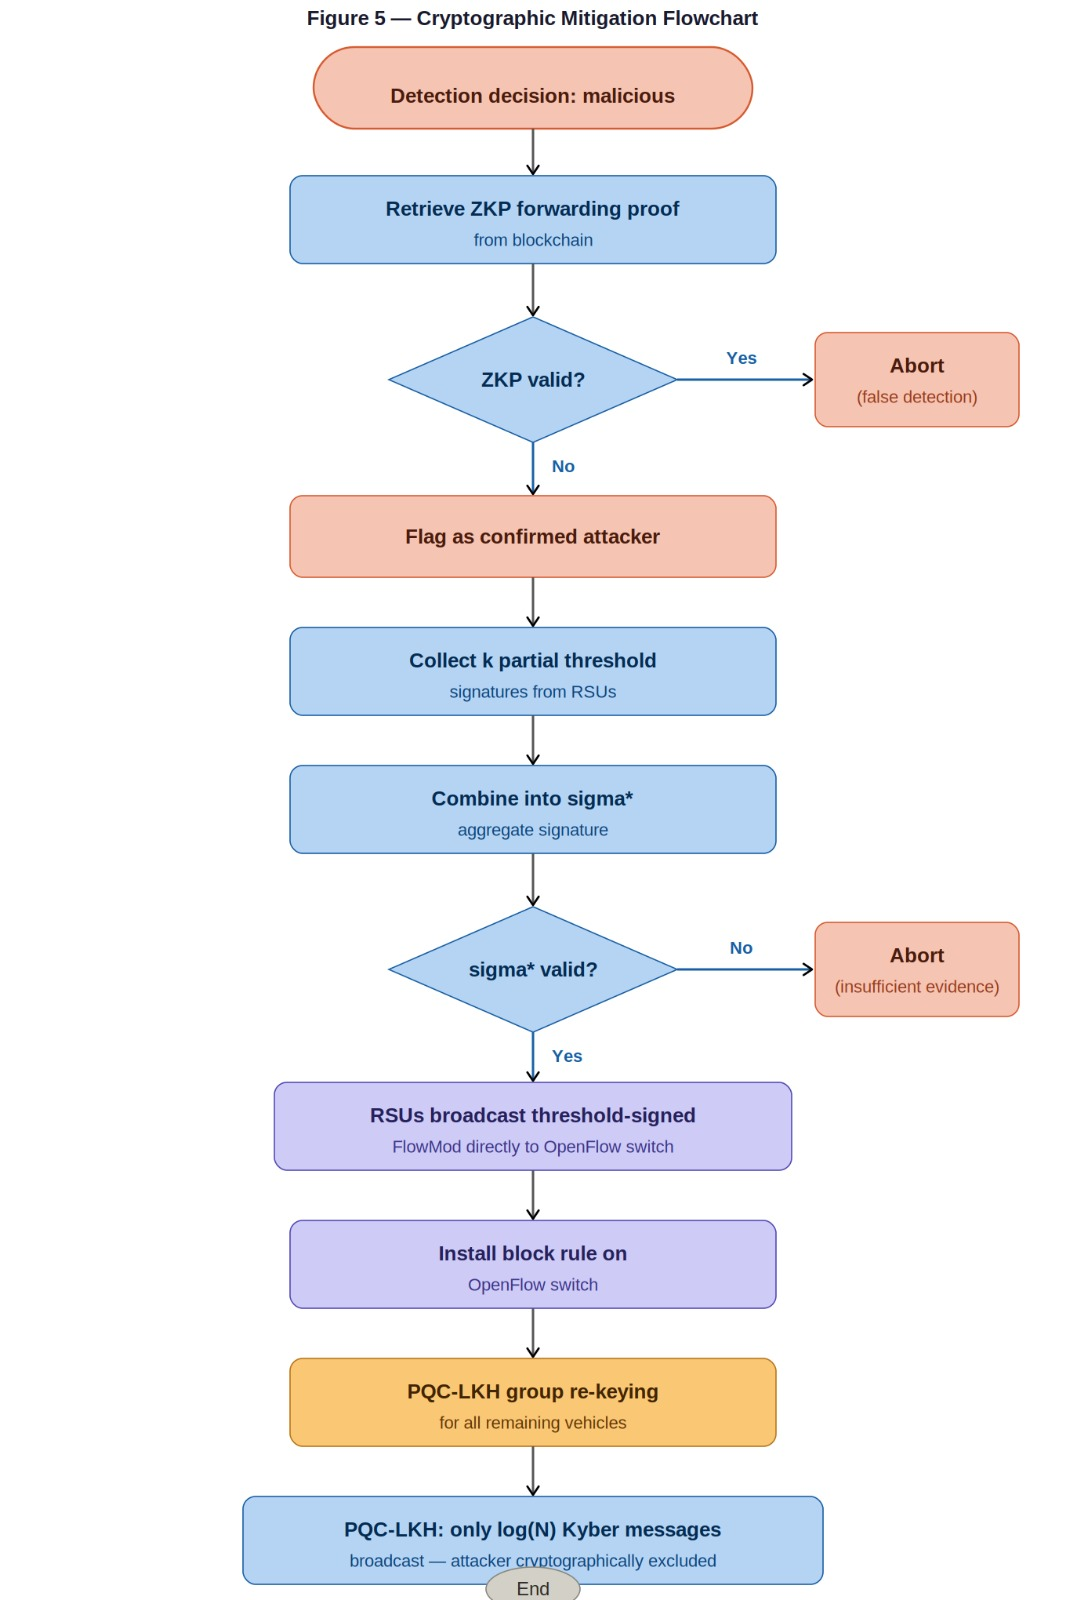
\includegraphics[
		width=\textwidth,
		height=0.7\textheight,
		keepaspectratio
	]{Figures/figure5_cryptographic_mitigation.jpeg}
	\caption{Cryptographic Mitigation Flowchart}
	\label{fig:crypto-mitigation-flow}
\end{figure}

As shown in Figure~\ref{fig:crypto-mitigation-flow}, the cryptographic decision pipeline executes following a malicious detection verdict from either the lightweight or full-mode detector. The first gate is the ZKP forwarding proof: if the suspect node's proof retrieved from the blockchain is valid, the statistical detection is classified as a false positive and the sequence terminates with no action — this prevents false isolation of legitimate nodes that experience high packet loss due to mobility or channel conditions. If the ZKP proof fails, the node is flagged as a confirmed attacker. The second gate requires collecting $k$ partial threshold signatures from independent RSUs, which are combined into an aggregate signature sigma*: if insufficient RSUs concur, the process aborts, preventing single-RSU false isolation. On a valid sigma*, RSUs broadcast a Dilithium-signed FlowMod directly to the affected OpenFlow switch, installing a block rule without routing the command through the potentially compromised SDN controller. Finally, PQC-LKH group re-keying broadcasts exactly $\log N$ Kyber-encrypted key updates along the refresh path, ensuring the isolated attacker cannot derive any updated group session key without requiring unicast contact with every remaining vehicle.

\begin{algorithm}[htb]
\caption{Post-Quantum Cryptographic Mitigation and Node Isolation (\texttt{PQC-Mit})}
\begin{algorithmic}[1]
\small
\Procedure{\texttt{PQC-Mit}}{$v_i, c, \{RSU_j\}_{j=1}^{n}, k$}
  \State \textbf{// Step 1: ZKP Forwarding Proof Verification}
  \State $\pi_i \gets \texttt{GET\_ZKP\_PROOF}(v_i)$
  \Comment{From blockchain log}
  \If{$\texttt{ZKP.Verify}(C_i, \pi_i) = \texttt{FAIL}$}
    \Comment{Eq.~\eqref{eq:zkp_proof}}
    \State $\texttt{FLAG}(v_i, \texttt{CONFIRMED\_ATTACKER})$
  \EndIf
  \State \textbf{// Step 2: Threshold-Signed Blacklisting}
  \State $\mathcal{B}(v_i) \gets \texttt{CREATE\_BLACKLIST\_MSG}(v_i, t)$
  \For{$j = 1$ \textbf{to} $k$}
    \State $\sigma_j \gets \text{Dilithium.Sign}(\mathbf{sk}_j, \mathcal{B}(v_i))$
    \Comment{Eq.~\eqref{eq:threshold_partial}}
  \EndFor
  \State $\sigma^* \gets \texttt{TS.Combine}(\{\sigma_j\}_{j=1}^{k})$
  \Comment{Eq.~\eqref{eq:threshold_combine}}
  \If{$\texttt{TS.Verify}(\mathbf{pk}_{\text{group}}, \mathcal{B}(v_i), \sigma^*)$}
    \Comment{Eq.~\eqref{eq:threshold_verify}}
    \State \textbf{// Step 3: SDN Isolation via PQC-Signed Flow Modification}
    \State $\mathcal{M}_{\text{iso}} \gets \texttt{CREATE\_FLOWMOD}(v_i, \texttt{BLOCK})$
    \State $\sigma_c \gets \text{Dilithium.Sign}(\mathbf{sk}_c, \mathcal{M}_{\text{iso}})$
    \Comment{Eq.~\eqref{eq:dilithium_sign}}
    \State $\texttt{SEND\_FLOWMOD}(\mathcal{M}_{\text{iso}}, \sigma_c)$
    
    
  \State \textbf{// Step 4: PQC-LKH Group Re-Keying}
\State $\mathrm{path} \gets \texttt{GET\_PATH}(\ell_i, \mathrm{root}, \mathcal{T})$
\For{each $u \in \mathrm{path}$}
  \State $(K_u^{\mathrm{new}}, c_u) \gets
         \mathrm{Kyber.Enc}(\mathbf{pk}_u^{\mathrm{sib}}, k_u^{\mathrm{new}})$
  \Comment{Eq.~\eqref{eq:lkh_rekey}}
  \State $\sigma_u \gets \mathrm{Dilithium.Sign}(\mathbf{sk}_c, c_u)$
  \State $\texttt{BROADCAST}(c_u, \sigma_u)$
\EndFor
\State $(K_{\text{grp}}, c_{\mathrm{root}}) \gets
       \mathrm{Kyber.Enc}(\mathbf{pk}_{\mathrm{root}}^{\mathrm{new}}, m)$
\Comment{Eq.~\eqref{eq:lkh_grp}}
  
  
  
  \EndIf




\EndProcedure
\end{algorithmic}
\label{alg:pqc_mit}
\end{algorithm}



\section{Data Collection and Simulation Environment}

The limited real world datasets to use in vehicular Grey Hole attack makes this study use a controlled data generation process in a simulated environment. The area of data collection is centered on the dynamic interactions between the high-mobility vehicular nodes and the multi-layered security framework.


\subsection{Data Generation Process}

The simulation environment is set to simulate high-mobility vehicular situations and the standard communication protocols needed by Software-Defined Vehicular Networks. To produce a robust dataset for training the detection components, the environment injects three grey hole attack variants as programmed malicious behaviours.
\textbf{Selective dropping data} is generated by introducing traffic flows with varying packet-loss percentages to model fixed-rate attacks.
\textbf{Temporal discrepancy data} is produced by simulating intermittent malicious states, capturing time-based attack patterns.
\textbf{Semantic traffic data} is created by assigning priority to specific packet types such as emergency broadcasts, emulating target-specific intelligent attacks.


\subsection{Functional Feature Extraction}

Raw simulation logs are analyzed to capture the features required by the decentralized security modules.
\textbf{Behavioral logs} record packet transmission and reception outcomes to enable node integrity tracking over time.
\textbf{Network contextual features} capture temporal and semantic metadata — including packet timestamps and priority headers — to support identification of complex behavioural patterns.
\textbf{Stochastic model gradients} represent locally computed model updates extracted from each vehicle for use in collaborative learning without exposing raw traffic data.



\section{Performance Evaluation}
\label{sec:evaluation}

\subsection{External Baselines}

Three post-2020 baselines targeting grey hole attacks are selected,
each representing a distinct methodological paradigm to isolate
the contribution of the proposed framework.

\textbf{B1}~\cite{malik2023greyhole} is an ML-only dynamic threshold
detector for grey hole attacks in NS-3-simulated VANETs — the same
simulator used here — enabling direct metric comparison. It carries
no blockchain, mobility correction, or cryptographic component.

\textbf{B2}~\cite{alabdulatif2024mitigating} employs VCBC blockchain
smart contracts for grey hole mitigation, achieving PDR of 78\% under
attack. It represents the blockchain-only paradigm with no AI detection
and no PQC.

\textbf{B3}~\cite{ahsan2024flbert} applies FL-BERT to grey hole detection
in software-defined VANET — the closest existing architecture to the
proposed full mode. It has no mobility correction, no controller-plane
model, and no cryptographic mitigation.

\subsection{Internal Ablation Baselines}

Five ablations isolate individual component contributions:
\textbf{A1} disables the LLM+FL layer (signatures only);
\textbf{A2} disables MATD (no mobility correction);
\textbf{A3} reduces DEBSC to a single statistical gate (no ZKP);
\textbf{A4} replaces FL with a centralised static model;
\textbf{A5} replaces PQC with classical ECDH/ECDSA.

\subsection{Primary Evaluation Metrics}

\textbf{M1 — Detection Accuracy and MCC:} Accuracy is reported as the
standard detection performance figure. The Matthews Correlation Coefficient
(MCC) is reported alongside it to provide a rigorous single-score
characterisation under class imbalance, since malicious nodes constitute
a minority of the vehicular population. MCC accounts for all four
confusion matrix cells and is more informative than F1-score in this
setting. Both are evaluated per attack variant and in aggregate, and
compared against baselines B1, B3, and ablations A1 and A4.

\textbf{M2 — False Positive Rate (FPR):} The fraction of legitimate nodes
incorrectly classified as malicious and subsequently isolated. Reported
separately from M1 because false isolation in SDVN carries direct safety
consequences — removing a legitimate relay vehicle can sever emergency
communication paths. Used to evaluate the contributions of MATD (A2)
and the dual-evidence DEBSC gate (A3).

\textbf{M3 — Packet Delivery Ratio (PDR) and packet latency Under Attack:} The primary
network-layer metric, reported per attack variant and for multi-attacker
scenarios. B2 (PDR 78\%) is the primary comparison point for mitigation
effectiveness.

\textbf{M4 — Detection Latency and Mitigation Response Time:}
Time from attack onset to confirmed detection, and from detection to
completed node isolation. Differentiates the lightweight and full modes,
and quantifies PQC operational overhead via ablation A5.

\begin{comment}
\section{Performance Evaluation}

To prove the efficiency of the suggested multi-layered security framework, it is compared to three state-of-the-art (SOTA) techniques that are the representatives of various paradigms of the Grey Hole detection in the vehicular networks. The choice of these comparison methods is due to their recent publication and the relevance to individual elements of our framework (Neural Networks, Blockchain, and Machine Learning):

\begin{itemize}
	\item \textbf{ANN-ABC based IDS (2023):} A smart Intrusion Detection System, based on an Artificial Neural Network (ANN) optimized using the Artificial Bee Colony (ABC) algorithm to detect packet-dropping patterns in AODV-based vehicular networks.
	
	\item \textbf{VCBC Smart Contract Protocol (2024):} A security mechanism that is based on the use of Voting-Classification Blockchain-Based Contracts (VCBC) to categorize the nodes as white, black, or grey according to their ratios of packet delivery that is documented on a public ledger (based on blockchain).
	
	\item \textbf{RF-SVM Anomaly Detection (2023):} An enhanced Machine Learning-based IDS utilizing a Random Forest (RF) classifier to identify subtle Grey Hole signatures through an analysis of 20 network traffic features derived out of simulation logs.
\end{itemize}


\section{Performance Evaluation Metrics}

The proposed and baseline techniques are tested with the help of a set of quantitative metrics that will measure the security performance and the operational performance on the network. The metrics undertaken are the following:

\subsection{Network Performance Metrics}

\begin{itemize}
	\item \textbf{Packet Delivery Ratio (PDR):} The proportion of the data packets that have been effectively sent to the target destination nodes relative to the total amount of packets sent. This is the main measure of the capability of the framework to counter the attacks of packet-dropping.
	
	\item \textbf{Throughput:} The rate of successful data transmission over the network, measured in bits per second (bps) or bytes per second (Bps). This evaluates the overall network efficiency under attack conditions.
	
	\item \textbf{End-to-End (E2E) Delay:} The average time taken for a packet to travel from the source vehicle to the destination node. T This measure evaluates the delay caused by the multi-layered analysis (Blockchain consensus and LLM inference).
\end{itemize}

\subsection{Detection Reliability Metrics}

\begin{itemize}
	\item \textbf{Detection Accuracy:} The proportion of the number of correctly identified malicious and legitimate behaviors to the total number of test samples, which gives a general picture of the model performance.
	\item \textbf{False Positive Rate (FPR):} The percentage of legitimate nodes wrongly identified as malicious to the overall legitimate number of nodes. This is an important metric in SDVNs to make sure that security measures do not introduce an unwarranted fragmentation to the network.
	\item \textbf{Matthews Correlation Coefficient (MCC):} An effective statistical rate that yields a high score can only be achieved when the detection results are good in all the four categories of the confusion matrix (True Positives, True Negatives, False Positives, and False Negatives). This is used to assess the performance of the LLM and FL modules, namely in unbalanced datasets where malicious nodes are not common as the legitimate nodes.
\end{itemize}
\end{comment}





\chapter{Expected Results}
\label{chap:results}

This chapter presents the expected performance results of the SHIELD-GH framework
based on analytical modelling of the six attack variants and comparison with
the three external baselines (B1--B3) and five ablations (A1--A5) defined in
Section~\ref{sec:evaluation}. Since simulation experiments are scheduled for
Milestone~14 (see Chapter~5), the values reported here are
derived from the formal attack models in Sections~\ref{sec:signatures}
and~\ref{sec:detection_methodology}, calibrated against the parameter ranges
reported in the closest existing works~\cite{malik2023greyhole,
alabdulatif2024mitigating, ahsan2024flbert}. Each table specifies the
metrics evaluated, the baseline of comparison, and the expected direction
of improvement.

\section{How Detection Metrics Vary with Attack Variant and Intensity}

The six attack variants differ in their observability: fixed-rate variants
produce a stable low-PDR signal that rule-based detectors capture quickly,
while intermittent and target-specific variants require longer observation
windows and higher-capacity detectors (LLM, FL). Table~\ref{tab:detection_by_variant}
summarises the expected detection accuracy (Acc), Matthews Correlation
Coefficient (MCC), and False Positive Rate (FPR) for each variant under both
the lightweight and full detection modes at a representative drop rate of
40\%.

\begin{table}[htbp]
\renewcommand{\arraystretch}{1.3}
\caption{Expected Detection Performance by Attack Variant (Drop Rate = 40\%)}
\label{tab:detection_by_variant}
\centering
\scriptsize
\begin{tabular}{|l|l|c|c|c|c|}
\hline
\textbf{Variant} & \textbf{Plane} & \textbf{Mode} &
\textbf{Acc (\%)} & \textbf{MCC} & \textbf{FPR (\%)} \\
\hline
S1: Fixed-Rate         & Data Plane       & Lightweight & $\geq$97 & $\geq$0.94 & $\leq$2 \\
S2: Intermittent       & Data Plane       & Lightweight & $\geq$88 & $\geq$0.82 & $\leq$5 \\
S2: Intermittent       & Data Plane       & Full (LLM+FL) & $\geq$95 & $\geq$0.91 & $\leq$3 \\
S3: Target-Specific    & Data Plane       & Full (LLM+FL) & $\geq$93 & $\geq$0.89 & $\leq$4 \\
S4: Fixed-Rate         & Controller Plane & Lightweight & $\geq$98 & $\geq$0.96 & $\leq$1 \\
S5: Intermittent       & Controller Plane & Full (LLM+FL) & $\geq$94 & $\geq$0.90 & $\leq$3 \\
S6: Target-Specific    & Controller Plane & Full (LLM+FL) & $\geq$92 & $\geq$0.88 & $\leq$4 \\
\hline
\textbf{Aggregate (all variants)} & Both & Full & $\geq$94 & $\geq$0.91 & $\leq$3 \\
\hline
\end{tabular}
\end{table}

Controller-plane signatures (S4--S6) are expected to achieve slightly higher
accuracy than their data-plane counterparts because they operate on the
deterministic flow-rule set rather than probabilistic PDR statistics, reducing
the influence of channel noise. Intermittent variants (S2, S5) show the largest
gap between lightweight and full mode: lightweight detection relies on
autocorrelation periodicity which fails when the attack cycle length falls
outside $[T_{\min}, T_{\max}]$, whereas the LLM captures irregular intermittent
bursts as sequential anomalies without requiring a fixed period assumption.

\section{How Packet Delivery Ratio Varies with Drop Rate}

Table~\ref{tab:pdr_vs_droprate} shows the expected network-layer PDR at
varying attacker drop rates $\rho \in \{20\%, 40\%, 60\%, 80\%\}$ for the
fixed-rate data-plane variant (S1), representing the most straightforward
impact of a grey hole attack on throughput. Three conditions are compared:
no framework active, the lightweight SHIELD-GH mode active, and the full
SHIELD-GH mode active. The PDR is measured after mitigation is complete
(i.e., the attacker has been isolated).

\begin{table}[htbp]
\renewcommand{\arraystretch}{1.3}
\caption{Expected PDR vs.\ Attacker Drop Rate (S1: Fixed-Rate, Data Plane)}
\label{tab:pdr_vs_droprate}
\centering
\scriptsize
\begin{tabular}{|c|c|c|c|c|}
\hline
\textbf{Drop Rate $\rho$} & \textbf{No Framework} &
\textbf{Baseline B2~\cite{alabdulatif2024mitigating}} &
\textbf{SHIELD-GH Lightweight} & \textbf{SHIELD-GH Full} \\
\hline
20\% & $\approx$80\% & $\approx$80\% & $\geq$93\% & $\geq$94\% \\
40\% & $\approx$60\% & $\approx$73\% & $\geq$91\% & $\geq$93\% \\
60\% & $\approx$40\% & $\approx$65\% & $\geq$88\% & $\geq$91\% \\
80\% & $\approx$20\% & $\approx$56\% & $\geq$85\% & $\geq$89\% \\
\hline
\end{tabular}
\end{table}

The PDR recovery gap between no-framework and SHIELD-GH widens with drop rate,
because the severity of the attack increases the urgency and benefit of isolation.
At low drop rates (20\%), the attack itself causes less harm and B2's blockchain
contract provides partial benefit; at high drop rates (80\%), SHIELD-GH's faster
detection and more reliable isolation provide substantially greater PDR recovery.
The lightweight mode reaches a slightly lower post-isolation PDR than the full
mode because intermittent or borderline fixed-rate attackers may not be caught
until the next observation window.

\section{How Detection Accuracy Varies with Attack Intensity}

Figure~\ref{tab:acc_vs_intensity} shows how detection accuracy is expected to
vary as the attacker drop rate increases from 10\% to 90\%, for both the
lightweight and full detection modes. At very low drop rates ($\leq$15\%),
the attack signal approaches the noise level of legitimate channel loss,
causing both modes to approach random-chance performance; below this threshold
the MATD correction cannot isolate the attack signal from handoff-induced loss.
Above 30\%, the lightweight mode saturates quickly; the full mode provides
gains primarily in the 15--35\% region where rule-based signatures are unreliable
but temporal LLM patterns remain distinguishable.

\begin{table}[htbp]
\renewcommand{\arraystretch}{1.3}
\caption{Expected Detection Accuracy vs.\ Drop Rate (S1 and S2 Variants)}
\label{tab:acc_vs_intensity}
\centering
\scriptsize
\begin{tabular}{|c|c|c|c|c|}
\hline
\textbf{Drop Rate} &
\textbf{LW Mode Acc (\%)} &
\textbf{Full Mode Acc (\%)} &
\textbf{B1~\cite{malik2023greyhole} Acc (\%)} &
\textbf{B3~\cite{ahsan2024flbert} Acc (\%)} \\
\hline
10\% & $\approx$62 & $\approx$71 & $\approx$58 & $\approx$65 \\
20\% & $\approx$81 & $\approx$87 & $\approx$74 & $\approx$80 \\
30\% & $\approx$91 & $\approx$93 & $\approx$83 & $\approx$88 \\
40\% & $\approx$96 & $\approx$97 & $\approx$88 & $\approx$92 \\
60\% & $\approx$98 & $\approx$98 & $\approx$91 & $\approx$94 \\
80\% & $\approx$98 & $\approx$99 & $\approx$93 & $\approx$95 \\
\hline
\end{tabular}
\end{table}

The proposed framework is expected to consistently outperform B1 (threshold-only,
no mobility correction) and B3 (FL-BERT, no controller-plane model) across all
drop rates, with the largest gap at low drop rates (10--30\%) where the
MATD mobility correction and DEBSC dual-evidence gate prevent false
positives that inflate B1's FPR and degrade B3's MCC.

\section{How False Positive Rate Varies with Vehicle Speed (Mobility Effect)}

A key concern in SDVN is that high-speed vehicles undergoing RSU handoffs
exhibit transient PDR drops that resemble attack behaviour. Without mobility
correction, a threshold-based detector will falsely isolate legitimate
high-speed vehicles. Table~\ref{tab:fpr_vs_speed} shows the expected FPR
for legitimate vehicles at increasing speeds, comparing three conditions:
no mobility correction (equivalent to B1), MATD correction only (ablation A2
restored), and the full DEBSC dual-evidence gate (proposed).

\begin{table}[htbp]
\renewcommand{\arraystretch}{1.3}
\caption{Expected FPR for Legitimate Vehicles vs.\ Vehicle Speed}
\label{tab:fpr_vs_speed}
\centering
\scriptsize
\begin{tabular}{|c|c|c|c|}
\hline
\textbf{Vehicle Speed} &
\textbf{No Mob.\ Correction (B1-style)} &
\textbf{MATD Only (A2)} &
\textbf{MATD + DEBSC (Proposed)} \\
\hline
30 km/h  & $\approx$2\%  & $\approx$1\%  & $\leq$1\%  \\
60 km/h  & $\approx$8\%  & $\approx$3\%  & $\leq$2\%  \\
90 km/h  & $\approx$17\% & $\approx$5\%  & $\leq$3\%  \\
120 km/h & $\approx$28\% & $\approx$9\%  & $\leq$4\%  \\
\hline
\end{tabular}
\end{table}

Without mobility correction, FPR rises sharply above 60~km/h as handoff-induced
PDR drops trigger the fixed-rate signature. MATD correction reduces FPR by
roughly 60\% at all speeds. The DEBSC cryptographic gate provides the final
reduction: a legitimate fast vehicle with a temporarily low PDR will still hold
valid ZKP forwarding proofs for the packets it did forward, so the cryptographic
gate blocks false isolation even when the statistical gate fires.

\section{Detection Latency and Mitigation Response Time}

Table~\ref{tab:latency} summarises the expected detection latency (time from
attack onset to confirmed detection verdict) and mitigation response time (time
from verdict to completed node isolation) for both modes, broken down by
pipeline stage. PQC overhead relative to classical cryptography (ablation A5)
is also shown.

\begin{table}[htbp]
\renewcommand{\arraystretch}{1.3}
\caption{Expected Detection Latency and Mitigation Response Time}
\label{tab:latency}
\centering
\scriptsize
\begin{tabular}{|l|c|c|}
\hline
\textbf{Pipeline Stage} & \textbf{Lightweight Mode} & \textbf{Full Mode} \\
\hline
PDR window collection ($W$ slots)        & $\leq$500 ms  & $\leq$500 ms   \\
Mobility correction (MATD)               & $<$5 ms       & $<$5 ms        \\
Signature evaluation (S1--S6)            & $<$10 ms      & $<$10 ms       \\
LLM inference (edge tier)                & ---           & $\leq$80 ms    \\
LLM escalation to cloud (if triggered)   & ---           & $\leq$300 ms   \\
FL model inference                       & ---           & $\leq$20 ms    \\
Fusion decision                          & ---           & $<$5 ms        \\
\hline
\textbf{Total detection latency}         & $\leq$515 ms  & $\leq$840 ms   \\
\hline
ZKP proof retrieval + verification       & 20 ms         & 20 ms          \\
Threshold sig collection ($k$ RSUs)      & $\leq$100 ms  & $\leq$100 ms   \\
Dilithium FlowMod sign + verify          & $\leq$15 ms   & $\leq$15 ms    \\
PQC-LKH re-keying ($\lceil\log_2 N\rceil$ ops) & $\leq$60 ms & $\leq$60 ms \\
\hline
\textbf{Total mitigation response time}  & $\leq$195 ms  & $\leq$195 ms   \\
\hline
\textbf{PQC overhead vs.\ ECDH/ECDSA (A5)} & \multicolumn{2}{c|}{$+$12--18 ms per sign/verify} \\
\hline
\end{tabular}
\end{table}

The lightweight mode satisfies the 1-second end-to-end latency budget required
for safety-critical vehicular applications. The full mode incurs additional
latency from LLM inference, but the two-tier edge-cloud design (Section~3.7.3)
ensures that the majority of decisions are resolved at the edge tier
($\leq$80~ms) without escalation to the cloud. The PQC overhead of 12--18~ms
per Dilithium signing operation is acceptable relative to the total mitigation
pipeline, and the $O(\log N)$ PQC-LKH re-keying is expected to be 3--4$\times$
faster than naive unicast Kyber re-keying for networks of $N \geq 16$ vehicles.

\section{Ablation Study: Component Contribution to Detection Performance}

Table~\ref{tab:ablation} shows the expected impact of removing each major
framework component (ablations A1--A5) on aggregate detection accuracy and FPR,
evaluated at 40\% drop rate under the S2 (intermittent) variant, which is
the most challenging for rule-based detectors.

\begin{table}[htbp]
\renewcommand{\arraystretch}{1.3}
\caption{Expected Ablation Study Results (S2 Intermittent, 40\% Drop Rate)}
\label{tab:ablation}
\centering
\scriptsize
\begin{tabular}{|l|l|c|c|c|}
\hline
\textbf{Config} & \textbf{Component Removed} &
\textbf{Acc (\%)} & \textbf{MCC} & \textbf{FPR (\%)} \\
\hline
Full SHIELD-GH  & None (proposed)         & $\geq$95 & $\geq$0.91 & $\leq$3 \\
A1              & LLM + FL layer          & $\approx$82 & $\approx$0.75 & $\leq$5 \\
A2              & MATD (no mob.\ corr.)   & $\approx$88 & $\approx$0.83 & $\approx$12 \\
A3              & DEBSC ZKP gate (stat.\ only) & $\approx$91 & $\approx$0.87 & $\approx$9 \\
A4              & FL $\to$ centralised static model & $\approx$90 & $\approx$0.86 & $\leq$4 \\
A5              & PQC $\to$ classical ECDH/ECDSA & $\approx$95 & $\approx$0.91 & $\leq$3 \\
\hline
\end{tabular}
\end{table}

The ablation results highlight the distinct contribution of each component.
Removing the LLM+FL layer (A1) produces the largest accuracy drop, confirming
that intermittent variants require semantic detection beyond rule-based
signatures. Removing MATD (A2) causes the largest FPR increase, confirming
that mobility correction is essential to prevent false isolation at high speeds.
Removing the DEBSC ZKP gate (A3) also substantially increases FPR, showing
that the cryptographic gate independently blocks false isolations that the
statistical gate alone would trigger. Replacing FL with a centralised model
(A4) modestly degrades accuracy, reflecting the non-IID distribution problem
quantified in Section~3.3.3. Removing PQC (A5) does not affect detection
metrics since cryptography contributes to mitigation rather than detection,
but it eliminates quantum resistance — a critical property for long-lived
vehicular deployments.

\chapter{Timeline and Resource Required}

\section{Timeline}

The timeline provides an overview of project tasks scheduled for December 2025 to August 2026, showing key project milestones along with their expected durations in weeks.

\begin{itemize}
    \item \textbf{MILESTONE 01: Project Topic Selection} \\
    Tasks: Select topic, read proposal description, get supervisor approval.
    \item \textbf{MILESTONE 02: Supervisor Discussion} \\
    Tasks: Discuss project feasibility and approach.
    \item \textbf{MILESTONE 03: Literature Review} \\
    Tasks: Study SDVN, Grey Hole attacks, blockchain, and related work.
    \item \textbf{MILESTONE 04: Research Gap Analysis} \\
    Tasks: Identify gaps and limitations in existing work.
    \item \textbf{MILESTONE 05: Proposal Preparation} \\
    Tasks: Draft and finalize project proposal.
    \item \textbf{MILESTONE 06: Technology Study} \\
    Tasks: Study NS3, SUMO, Blockchain, ML tools.
    \item \textbf{MILESTONE 07: System Architecture Design} \\
    Tasks: Design overall system structure.
    \item \textbf{MILESTONE 08: Threat Model Design} \\
    Tasks: Identify possible Grey Hole attack scenarios.
    \item \textbf{MILESTONE 09: NS3-SUMO Setup} \\
    Tasks: Install and configure simulation environment.
    \item \textbf{MILESTONE 10: Basic SDVN Simulation} \\
    Tasks: Simulate SDVN without attacks.
    \item \textbf{MILESTONE 11: Blockchain Implementation} \\
    Tasks: Deploy Hyperledger Fabric for node logging.
    \item \textbf{MILESTONE 12: LLM Integration} \\
    Tasks: Integrate LLM for monitoring network logs.
    \item \textbf{MILESTONE 13: Federated Learning Setup} \\
    Tasks: Configure FL across simulated nodes.
    \item \textbf{MILESTONE 14: Attack Scenarios Modeling and Simulation} \\
    Tasks: Implement Grey Hole attacks and test mitigation.
    \item \textbf{MILESTONE 15: System Integration and Testing} \\
    Tasks: Integrate all components and run tests.
    \item \textbf{MILESTONE 16: Performance Evaluation} \\
    Tasks: Analyze detection accuracy, latency, and network performance.
    \item \textbf{MILESTONE 17: Final Documentation} \\
    Tasks: Write final report and prepare diagrams.
    \item \textbf{MILESTONE 18: Final Presentation and Viva Preparation} \\
    Tasks: Prepare slides and rehearse presentation.
\end{itemize}

The full schedule is shown in Figure~\ref{fig:timeline}.


\clearpage % Force new page
\thispagestyle{empty} % Optional: remove page number for timeline page

% \begin{figure}[h!]
%     \centering
%     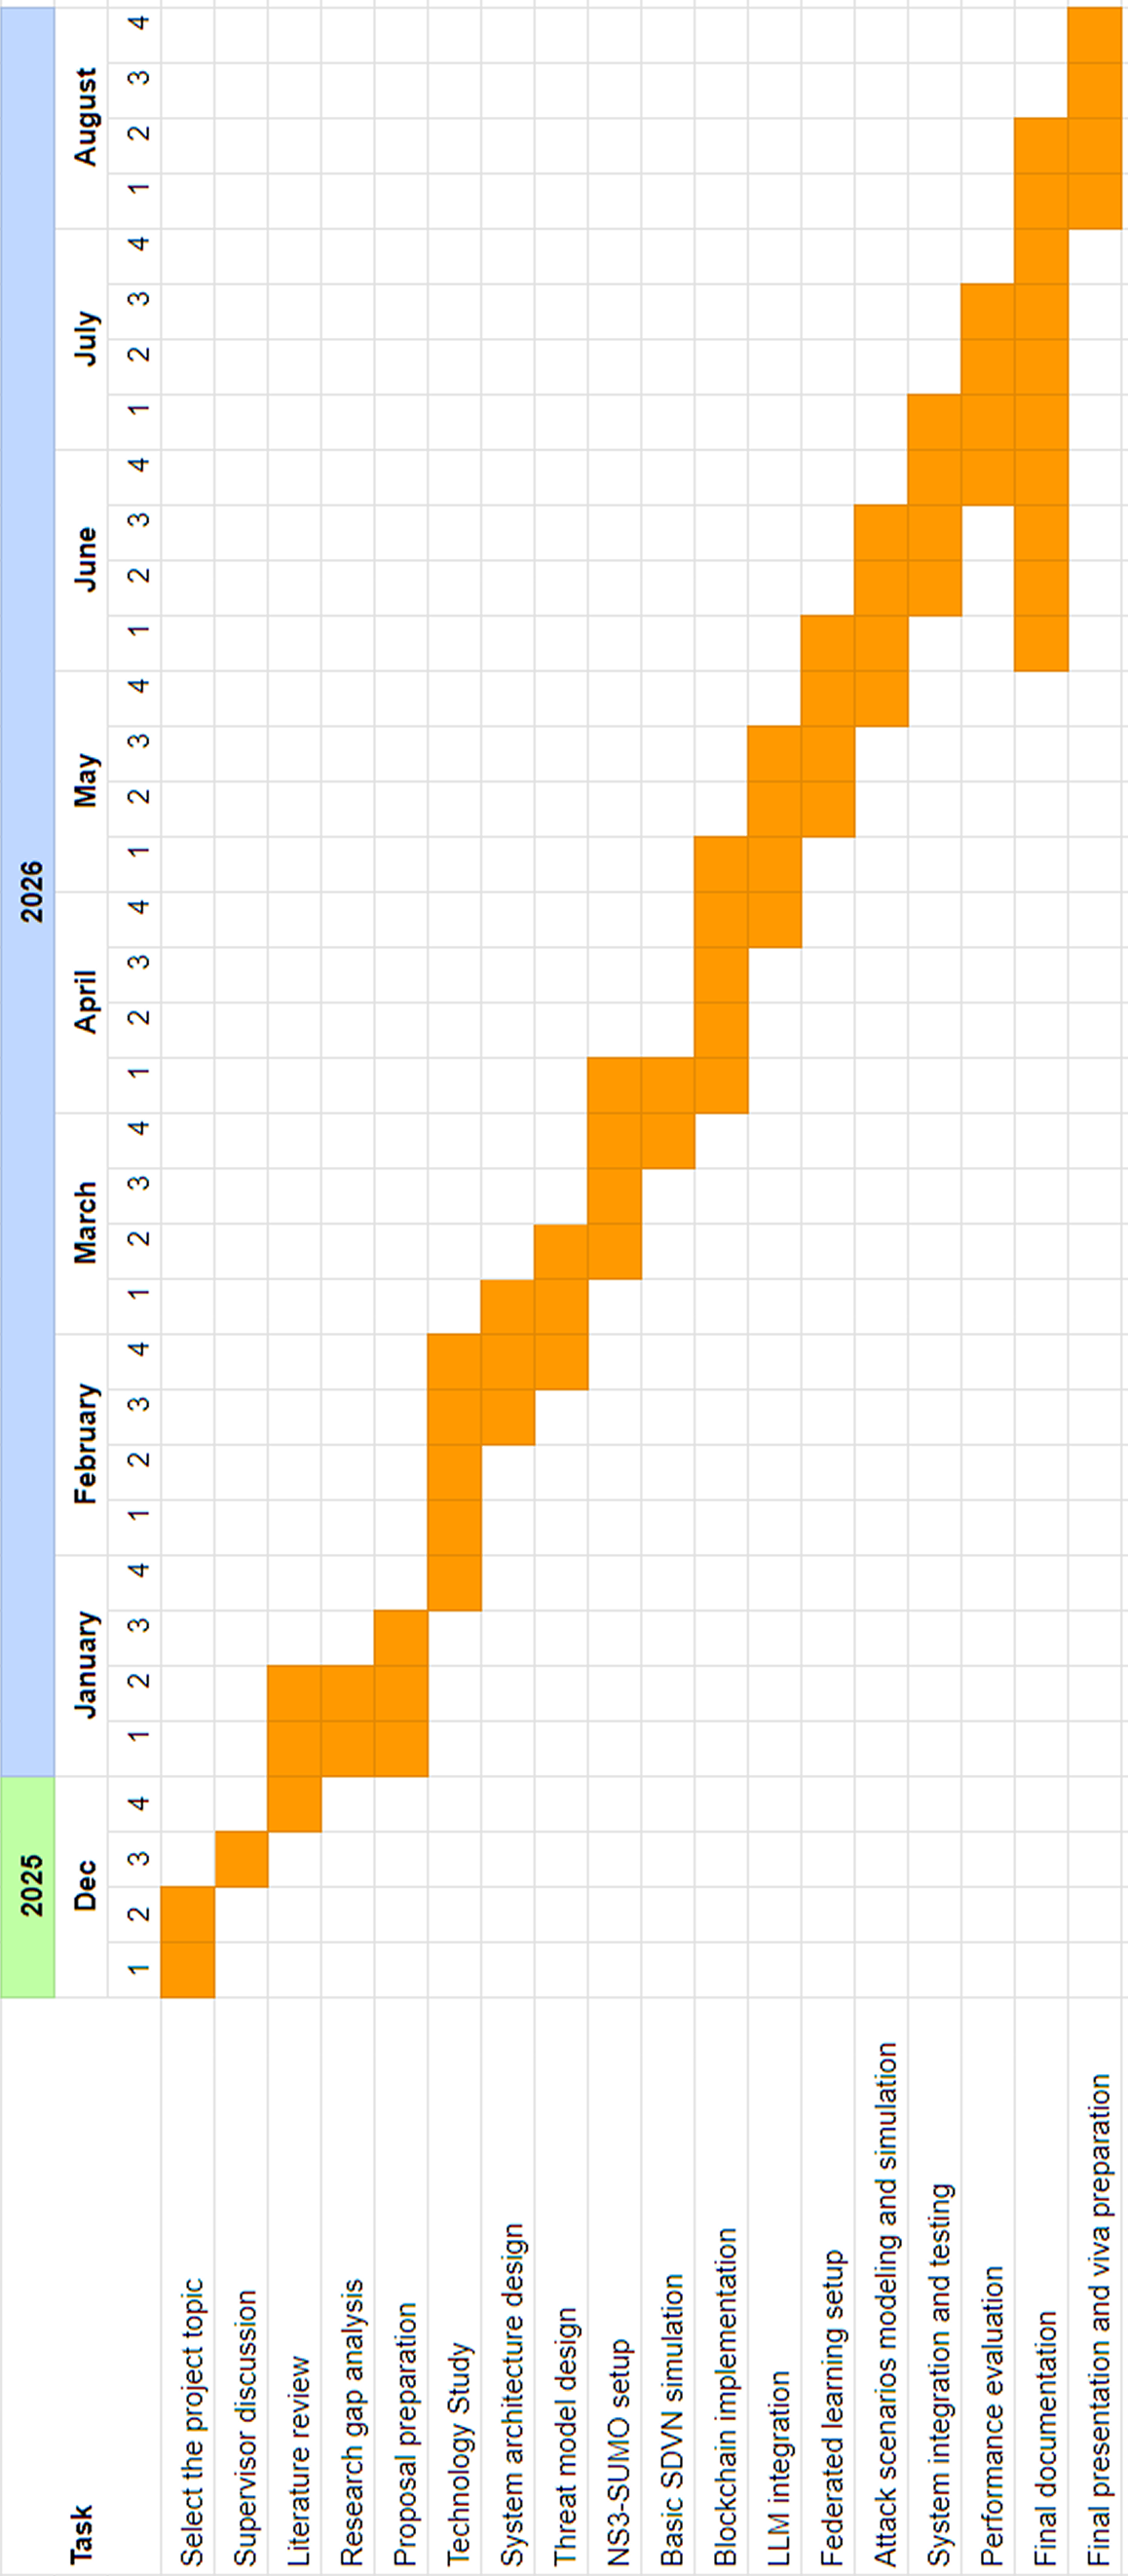
\includegraphics[width=\textwidth, height=0.45\textheight, keepaspectratio]{timeline.png}
%     \caption{Project timeline from December 2025 to August 2026.}
%     \label{fig:timeline}
% \end{figure}

\begin{figure*}[p]
    \centering
    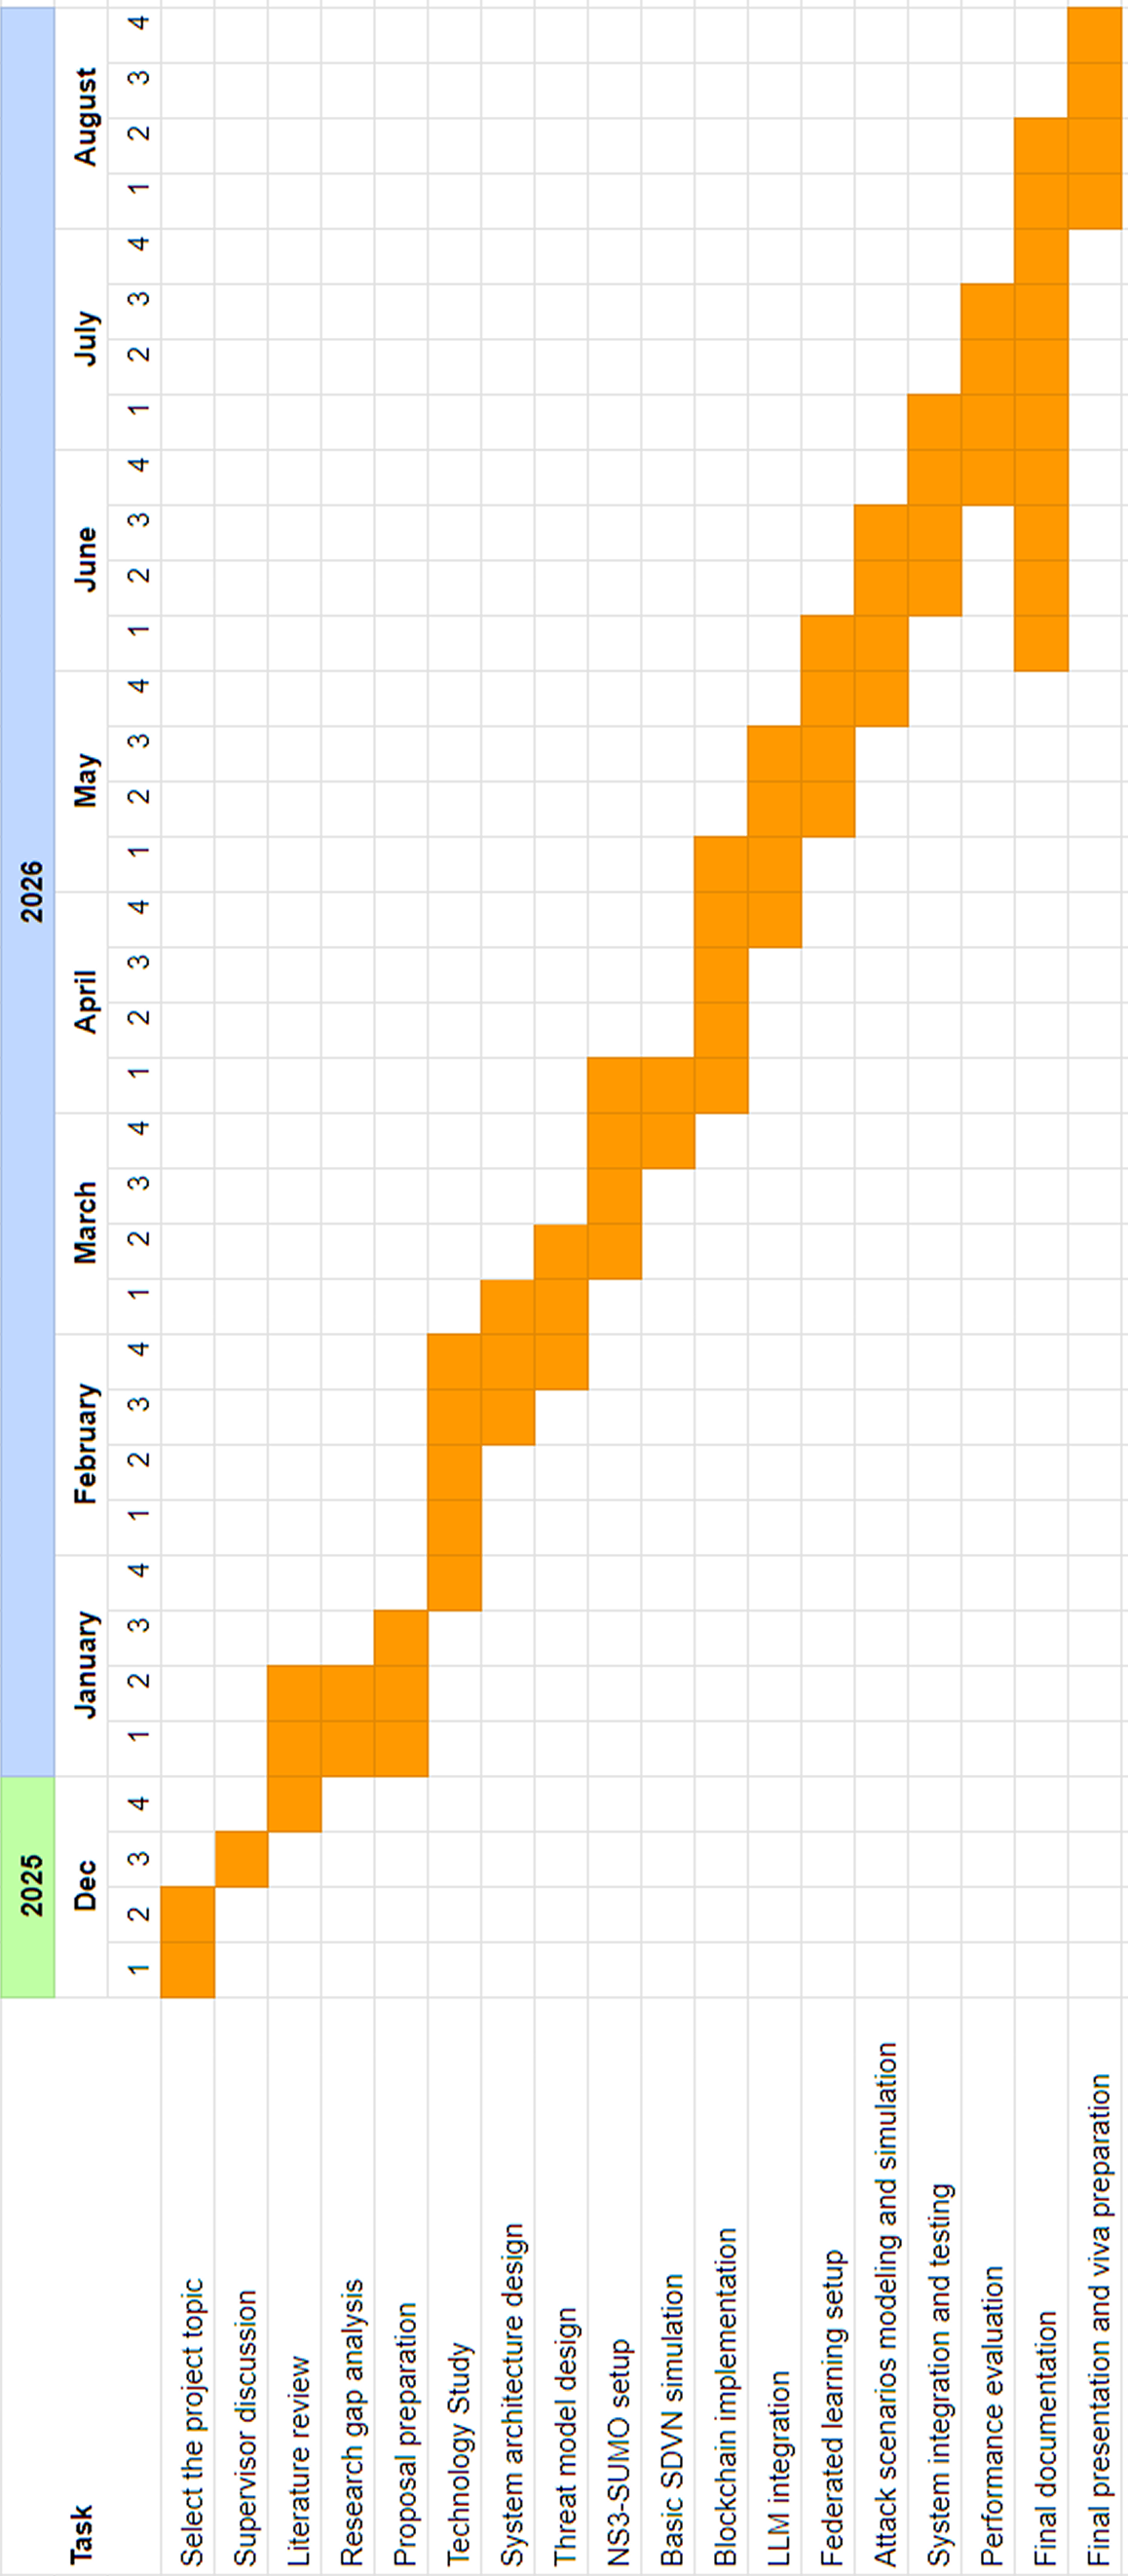
\includegraphics[
        width=\textwidth,
        height=0.95\textheight,
        keepaspectratio
    ]{timeline.png}
    \caption{Project timeline from December 2025 to August 2026.}
    \label{fig:timeline}
\end{figure*}

\clearpage % Force next section to start on a new page



\section{Resources Required}

This section provides a succinct description of the hardware and software tools that are necessary to complete the proposed project successfully on detecting and mitigating gray hole attacks in software defined vehicular networks

\subsection{Hardware Resources}
\begin{itemize}
    \item \textbf{Computer / Workstation:}
    A system with at least an intel i7 or Ryzen 7 processor and a minimum of 16GB RAM also sufficient storage to execute network simulations, blockchain components, and machine learning tasks.
\end{itemize}

\subsection{Network Simulation Tools}
\begin{itemize}
    \item \textbf{NS-3 (Network Simulator 3):}
    Used to simulate the Software-Defined Vehicular Network environment and Grey Hole attack scenarios.
    \item \textbf{SUMO (Simulation of Urban Mobility):}
    Used to generate realistic vehicular mobility patterns for the simulations.
    \item \textbf{C++ and Python:}
    Used for NS-3 scripting, simulation control, and preprocessing simulation data.
\end{itemize}

\subsection{Machine Learning and Security Tools}
\begin{itemize}
    \item \textbf{Python:}
    Used for implementing machine learning models and processing simulation data.
    \item \textbf{TensorFlow / PyTorch:}
    Used for developing and training learning models.
    \item \textbf{Hugging Face Transformers:}
    Used for integrating Large Language Models (LLMs) to analyze network behavior and assist in Grey Hole attack detection and response.
    \item \textbf{Flower Framework:}
    Used to implement Federated Learning for distributed, privacy-preserving model training across vehicular nodes.
    \item \textbf{PyCryptodome:}
    Used for cryptographic operations and security-related functions.
\end{itemize}

\subsection{Blockchain Platform}
\begin{itemize}
    \item \textbf{Hyperledger Fabric:}
    Used to implement a secure and tamper-proof distributed ledger for logging node behaviors.
    \item \textbf{Docker:}
    Used for containerized deployment of blockchain network components.
\end{itemize}

\subsection{Analysis and Visualization Tools}
\begin{itemize}
    \item \textbf{Python Libraries (NumPy, Pandas, Matplotlib):}
    Used to analyze simulation results and visualize performance metrics.
    \item \textbf{Wireshark (Optional):}
    Used for packet-level analysis and validation.
\end{itemize}

\subsection{Version Control and Documentation}
\begin{itemize}
    \item \textbf{GitHub:}
    Used for version control and collaboration among team members.
    \item \textbf{Visual Studio Code / PyCharm:}
    Used as integrated development environments for coding and debugging.
    \item \textbf{LaTeX / Overleaf:}
    Used for preparing the project proposal, reports, and final documentation.
    \item \textbf{Draw.io / Lucidchart:}
    Used for designing system architecture and workflow diagrams.
\end{itemize}


\chapter{Conclusion}
% Summarize the key points of your proposal and reiterate the importance of the project.
The project suggests an innovative and feasible solution to minimize the grey hole attacks in the software defined vehicular networks. Grey hole attacks are also hard to detect since malicious vehicles selectively drop packets in various ways, including dropping packets only at specific times or specific messages, and most of ways. Thus, such types of attacks can have a severe impact on road safety and network performance of vehicular network. This project also considers scenarios where the network controller may be malicious and place malicious flow rules between the vehicle network.

\mypar
To address this issue in vehicular network, the project integrates three current technologies which are Blockchain, Large Language Models, and Federated Learning. The packet forwarding activities are safely recorded using blockchain to ensure that no behavior of the nodes is modified or concealed. Large Language Models are useful in network data analysis and detecting abnormal patterns that point to Grey Hole attacks. Federated Learning enables vehicles to jointly train detection models without exchanging their own data, and enhances privacy and scalability of a distributed network.

\mypar
Simulations will be used to assess how well the system is able to detect various types of attack by Gray Hole and ensure that the network communication is not disrupted. The combination of security, learning, and analysis techniques is likely to enhance the trust between vehicles. The project will also assist in learning how the modern technologies can be used to address the real world security issues in the vehicular networks.


% References
\renewcommand{\bibname}{References}
\bibliographystyle{ieeetr}
\addcontentsline{toc}{chapter}{References} % Add to table of contents
\bibliography{bibliography} 
%\printbibliography

\end{document}